% !TEX TS-program = XeLaTeX
% !TEX encoding = UTF-8 Unicode

%%%%%%%%%%%%%%%%%%%%%%%%%%%%%%%%%%%%%%%%%%%%%%%%%%%%%%%%%%%%%%%%%%%%%% 
% 
%	大连理工大学博士论文 XeLaTeX 模版 —— 主文件 main.tex
% 版本:0.82
% 最后更新:2012.05.09
% 修改者:Yuri (E-mail: yuri_1985@163.com)
% 修订者:whufanwei(E-mail: dutfanwei@qq.com)
% 编译环境1:Ubuntu 12.04 + TeXLive 2011 + Emacs
% 编译环境2:Windows 7 + CTeX v2.9.2.164 + WinEdit
% 
%%%%%%%%%%%%%%%%%%%%%%%%%%%%%%%%%%%%%%%%%%%%%%%%%%%%%%%%%%%%%%%%%%%%%% 
\documentclass[12pt,a4paper,openany,twoside]{book}

% 字体配置文件
\input{setup/fonts}

% Used packages
%%%%%%%%%%%%%%%%%%%%%%%%%%%%%%%%%%%%%%%%%%%%%%%%%%%%%%%%%%%%%%%%%%%%%%%%%%%%%%%%
%
%   Doctoral Dissertation of Dalian University of Technology
%   By Jie Li and Ahmedin Mohammed Ahmed on the work of Hui Wang
%   package.tex
%   Version: 0.1
%   Update: 2014-04-16
%   Environment: Windows 8.1 + CTeX 2.9.2.164 + WinEdt 7.0
%   欢迎使用,如有任何意见和建议请发送邮件至 yuri_1985@163.com,感谢您的支持!
%
%%%%%%%%%%%%%%%%%%%%%%%%%%%%%%%%%%%%%%%%%%%%%%%%%%%%%%%%%%%%%%%%%%%%%%%%%%%%%%%%

% 版面控制
\usepackage[body={16.1true cm,22.0true cm}]{geometry}   %论文版芯161mm×220mm(不包括页眉页脚)
\usepackage{indentfirst}    % 首行缩进宏包
\usepackage[sf]{titlesec}   % 控制标题的宏包
\usepackage{titletoc}       % 控制目录的宏包
\renewcommand\bibname{References}
\usepackage{fancyhdr}       % 自定义页眉页脚
\usepackage{fancyref}       % 引用链接属性
\usepackage{cite}           % 支持引用的宏包
\usepackage[perpage,symbol]{footmisc}   % 脚注控制
\usepackage{layouts}        % 打印当前页面格式的宏包
\usepackage{paralist}       % 一种换行不缩进的列表格式,用 asparaenum 或者 inparaenum 环境
\usepackage[numbers]{natbib}         % 参考文献
\usepackage{fancyvrb}       % 原样输出
%\usepackage{listings}   % 粘贴源代码
%\usepackage[shortlabels]{enumitem}
% 字体
\usepackage{CJK}        % 中文支持宏包
\usepackage{amsmath}    % AMS 宏包,包含一些常用的数学字体和符号,
\usepackage{amssymb}    % 如果你引用一些不常见的字体宏包可能会与此发生冲突,请考虑略去。
\usepackage[mathscr]{eucal} % to replace the following commented package
%\usepackage{mathrsfs}   % 一种常用于定义泛函算子的花体字母,只有大写。
\usepackage[amsmath,thmmarks,hyperref]{ntheorem} % 定理类环境宏包,其中 amsmath 选项用来兼容 AMS的宏包
%\usepackage[amsmath,thmmarks]{ntheorem}
\usepackage{type1cm}    % 控制字体的大小
\usepackage{bm}         % 处理数学公式中的黑斜体的宏包
%\usepackage{fourier}    % 一种和Times类似的字体
\usepackage{txfonts}   % 如果你希望和 Word 的默认值保持一致,请使用此宏包
\usepackage{helvet}
\newcommand{\BigO}[1]{\ensuremath{\operatorname{O}\bigl(#1\bigr)}}
\usepackage[table]{xcolor}
\newcommand{\me}{\mathrm{e}}

\usepackage[T1]{fontenc}
\usepackage{makecell}
\renewcommand{\rothead}[3][90]{\makebox[9mm][c]{\rotatebox{#1}{\makecell[c]{#2}}}}%
\usepackage{multirow}
\usepackage{rotating,tabularx}

% 图形
\usepackage{graphicx}   % 这里引用 graphicx 宏包时没有图形驱动选项,所以请在引用图片时务必给出后缀名
\usepackage{subfigure}  % 插入子图形
\usepackage{color}      % 支持彩色
\usepackage[below]{placeins}    % 浮动图形控制宏包
\usepackage{picinpar}   % 图文混排用宏包
%\usepackage{floatflt}  % 图文混排用宏包
\usepackage{rotating}   % 图形和表格的控制
\usepackage[subfigure]{ccaption}    % 浮动图形和表格标题样式,支持插图表格的双语标题
\usepackage{setspace}   % 定制表格和图形的多行标题行距!!
\usepackage[ruled,vlined]{algorithm2e}
\usepackage[font={small}]{caption}

% 其他
\usepackage{calc}   % 在 tex 文件中具有一些计算功能,主要用在页面控制。
\usepackage{ccmap}      % 使pdfLatex生成的文件支持复制等
%\usepackage[pdftex,
            %CJKbookmarks=true,
            %bookmarksnumbered=true,
            %bookmarksopen=true,
            %colorlinks=true,
            %citecolor=black,
            %linkcolor=black,
            %anchorcolor=green,
            %urlcolor=magenta,
            %breaklinks=true
            %]{hyperref} % 生成有书签和超链接的 pdf
\usepackage[xetex,
	bookmarksnumbered=true,
	bookmarksopen=true,
	colorlinks=true,
	% pdfborder={0 0 1},
	citecolor=blue,
	linkcolor=blue,
	anchorcolor=green,
	urlcolor=magenta,
	breaklinks=true,
	CJKbookmarks=true,
	]{hyperref}















% Settings about Table of Contents (Jie Li and Ahmedin on the work of Hui Wang)
%以下由王辉增加(2012年12月16日),主要是修改英文目录和图标目录
%Revision 1: 目录中的点的稠密程度
\makeatletter
\def\@dotsep{0.3}%就在这儿改,把2改成其他什么,默认是4.5,就是点之间距离为4.5mu
\makeatother



%Revision 2: Formatting Table of Contents in Chinese and English
%Font
\titlecontents{chapter}[10mm]
{\fontsize{12pt}{15pt}}
{\contentslabel{4em}}
{}
{\titlerule*{.}\contentspage}
%
\titlecontents{section}[12mm]
{\fontsize{12pt}{15pt}}
{\contentslabel{2em}}
{}
{\titlerule*{.}\contentspage}
%
\titlecontents{subsection}[23mm]
{\fontsize{12pt}{15pt}}
{\contentslabel{3em}}
{}
{\titlerule*{.}\contentspage}

%Indent
\dottedcontents{chapter}[0.32cm]{\vspace{0.2em}}{1.0em}{5pt}
\dottedcontents{section}[1.32cm]{}{1.8em}{5pt}
\dottedcontents{subsection}[2.32cm]{}{2.7em}{5pt}
\dottedcontents{subsubsection}[3.32cm]{}{3.4em}{5pt}

%Revision 3: Content in English
\makeatletter
\newcommand\engcontentsname{\hfill CONTENTS \hfill}
%\newcommand\engcontentsname{CONTENTS}
\newcommand\tableofengcontents{%
    \if@twocolumn
      \@restonecoltrue\onecolumn
    \else
      \@restonecolfalse
    \fi
    \chapter*{\engcontentsname
        \@mkboth{%
           \MakeUppercase\engcontentsname}{\MakeUppercase\engcontentsname}}%
    \@starttoc{toe}% !!!!Define a new contents!!!!
    \if@restonecol\twocolumn\fi
    }
\newcommand\addengcontents[2]{%
    \addcontentsline{toe}{#1}{\protect\numberline{\csname the#1\endcsname}#2}}
\makeatother
\newcommand\echapter[1]{\addengcontents{chapter}{#1}}
\newcommand\esection[1]{\addengcontents{section}{#1}}
\newcommand\esubsection[1]{\addengcontents{subsection}{#1}}
\newcommand\esubsubsection[1]{\addengcontents{subsubsection}{#1}}




% The content
\begin{document}
\begin{CJK*}{GBK}{song}

% Format of text
%%%%%%%%%%%%%%%%%%%%%%%%%%%%%%%%%%%%%%%%%%%%%%%%%%%%%%%%%%%%%%%%%%%%%%%%%%%%%%%%
%
%   Doctoral Dissertation of Dalian University of Technology
%   By Jie Li and Ahmedin Mohammed Ahmed on the work of Hui Wang
%   format.tex
%   Version: 0.1
%   Update: 2014-04-16
%   Environment: Windows 8.1 + CTeX 2.9.2.164 + WinEdt 7.0
%   欢迎使用,如有任何意见和建议请发送邮件至 yuri_1985@163.com,感谢您的支持!
%
%%%%%%%%%%%%%%%%%%%%%%%%%%%%%%%%%%%%%%%%%%%%%%%%%%%%%%%%%%%%%%%%%%%%%%%%%%%%%%%%

%%%%%%%%%%%%%%%%%%%%%%%%%%%%%%%%%%%%%%%%%%%%%%%%%%%%%%%%%%%%%%%%%%%%%%%%%%%%%%%%80
% Settings of Pages
% 页面设置
%%%%%%%%%%%%%%%%%%%%%%%%%%%%%%%%%%%%%%%%%%%%%%%%%%%%%%%%%%%%%%%%%%%%%%%%%%%%%%%%80
% A4 纸张
\setlength{\paperwidth}{21.0cm}
\setlength{\paperheight}{29.7cm}

% Size of the content
% 设置正文尺寸大小
\setlength{\textwidth}{16.0cm}
\setlength{\textheight}{23.7cm}

% To make the content in the middle of the page
% 设置正文区在正中间
\newlength \mymargin
\setlength{\mymargin}{(\paperwidth-\textwidth)/2}
\setlength{\oddsidemargin}{(\mymargin)-1in}
\setlength{\evensidemargin}{(\mymargin)-1in}


% 设置正文区偏移量,奇数页向右偏,偶数页向左偏
\newlength \myshift
\setlength{\myshift}{0.35cm}     % 双面打印的奇偶页偏移值,可根据需要修改,建议小于 0.5 cm。
\addtolength{\oddsidemargin}{\myshift}
\addtolength{\evensidemargin}{-\myshift}
\setlength{\topmargin}{-0.75cm}
\setlength{\headheight}{0.50cm}
\setlength{\headsep}{0.90cm}
\setlength{\footskip}{1.47cm}

% Adjustment of equations
% 公式的精调
\allowdisplaybreaks[4]  % 可以让公式在排不下的时候分页排,这可避免页面有大段空白。

%下面这组命令使浮动对象的缺省值稍微宽松一点,从而防止幅度
%对象占据过多的文本页面,也可以防止在很大空白的浮动页上放置
%很小的图形。
\renewcommand{\textfraction}{0.15}
\renewcommand{\topfraction}{0.85}
\renewcommand{\bottomfraction}{0.65}
\renewcommand{\floatpagefraction}{0.60}

%%%%%%%%%%%%%%%%%%%%%%%%%%%%%%%%%%%%%%%%%%%%%%%%%%%%%%%%%%%%%%%%%%%%%%%%%%%%%%%%80
% Font and Size
% 字体字号定义
%%%%%%%%%%%%%%%%%%%%%%%%%%%%%%%%%%%%%%%%%%%%%%%%%%%%%%%%%%%%%%%%%%%%%%%%%%%%%%%%80
% Indent of Chinese
% 中文段落缩进和 ~ 字符替换
%\CJKindent                              % 首行缩进两个汉字
%\sloppy
%\CJKspace                              % 中英文混排的断行
%CJKtilde                               % 重新定义~,用~隔开中英文

% Chinese Font
% 中文字体
\newcommand{\song}{\CJKfamily{song}}    % 宋体 (Font of SONG)
\newcommand{\fs}{\CJKfamily{fs}}        % 仿宋 (Font of FANG SONG)
\newcommand{\kai}{\CJKfamily{kai}}      % 楷体
\newcommand{\hei}{\CJKfamily{hei}}      % 黑体
%\newcommand{\li}{\CJKfamily{li}}        % 隶书
%\newcommand{\you}{\CJKfamily{you}}      % 幼圆
%\newcommand{\xk}{\CJKfamily{STXingkai}}
% 字号

\newcommand{\yihao}{\fontsize{26pt}{39pt}\selectfont}               % 一号,1.5 倍行距
%\newcommand{\twentysix}{\fontsize{26pt}{39pt}\selectfont}               % 一号,1.5 倍行距
\newcommand{\xiaoyi}{\fontsize{24pt}{30pt}\selectfont}              % 小一,1.25倍行距
%\newcommand{\twentyfour}{\fontsize{24pt}{30pt}\selectfont}              % 小一,1.25倍行距
%\newcommand{\erhao}{\fontsize{22pt}{27.5pt}\selectfont}             % 二号,1.25倍行距
\newcommand{\xiaoer}{\fontsize{18pt}{22.5pt}\selectfont}            % 小二,1.25倍行距
\newcommand{\eighteen}{\fontsize{18pt}{27pt}\selectfont}            % 18 pt and 27 pt line space
\newcommand{\sanhao}{\fontsize{16pt}{20pt}\selectfont}              % 三号,1.25倍行距
\newcommand{\xiaosan}{\fontsize{15pt}{18.75pt}\selectfont}          % 小三,1.25倍行距
\newcommand{\daxiaosi}{\fontsize{12pt}{18pt}\selectfont}            % 小四,1.5 倍行距
\newcommand{\ltwelve}{\fontsize{12pt}{18pt}\selectfont}             % large twelve with 12pt, 18pt line space
\newcommand{\sihao}{\fontsize{14pt}{17pt}\selectfont}               % 四号,1.25倍行距
\newcommand{\fourteen}{\fontsize{14pt}{17pt}\selectfont}            % 14 pt and 17 pt line space
\newcommand{\thirteen}{\fontsize{13pt}{19.5pt}\selectfont}          % 13 pt, 19.5 pt line space
\newcommand{\xiaosi}{\fontsize{12pt}{15pt}\selectfont}              % 小四,1.25倍行距
\newcommand{\twelve}{\fontsize{12pt}{15pt}\selectfont}              % 小四(12 pt),1.25倍行距
\newcommand{\eleven}{\fontsize{11pt}{13.75pt}\selectfont}           % 11 pt, 13.75 line space
\newcommand{\dawu}{\fontsize{10.5pt}{18pt}\selectfont}              % 五号,1.75倍行距
\newcommand{\zhongwu}{\fontsize{10.5pt}{15pt}\selectfont}           % 五号,1.5 倍行距
\newcommand{\wuhao}{\fontsize{10.5pt}{10.5pt}\selectfont}           % 五号,单倍行距
\newcommand{\ten}{\fontsize{10pt}{10pt}\selectfont}                 % 五号,单倍行距
\newcommand{\xiaowu}{\fontsize{9pt}{9pt}\selectfont}                % 小五,单倍行距

% defaultfont 默认字体命令
\def\defaultfont{\renewcommand{\baselinestretch}{1.25}
\fontsize{12pt}{15pt}\selectfont}

% Font in Table of Content
% 设置目录字体和行间距
\def\defaultmenufont{\renewcommand{\baselinestretch}{1.22}
\fontsize{12pt}{12pt}}

% Content with fixed distance and underline
% 固定距离内容填入及下划线
\makeatletter
    \newcommand\fixeddistanceleft[2][1cm]{{\hb@xt@ #1{#2\hss}}}
    \newcommand\fixeddistancecenter[2][1cm]{{\hb@xt@ #1{\hss#2\hss}}}
    \newcommand\fixeddistanceright[2][1cm]{{\hb@xt@ #1{\hss#2}}}
    \newcommand\fixedunderlineleft[2][1cm]{\underline{\hb@xt@ #1{#2\hss}}}
    \newcommand\fixedunderlinecenter[2][1cm]{\underline{\hb@xt@ #1{\hss#2\hss}}}
    \newcommand\fixedunderlineright[2][1cm]{\underline{\hb@xt@ #1{\hss#2}}}
\makeatother
%%%%%%%%%%%%%%%%%%%%%%%%%%%%%%%%%%%%%%%%%%%%%%%%%%%%%%%%%%%%%%%%%%%%%%%%%%%%%%%%80
% Subtitles
% 标题相关
%%%%%%%%%%%%%%%%%%%%%%%%%%%%%%%%%%%%%%%%%%%%%%%%%%%%%%%%%%%%%%%%%%%%%%%%%%%%%%%%80
% Definition, Theorem, etc
% 定义、定理等环境
%\theoremstyle{plain}
%\theoremheaderfont{\hei\bf}
%\theorembodyfont{\song\rmfamily}
%\newtheorem{definition}{\hei 定义}[chapter]
%\newtheorem{example}{\hei 例}[chapter]
%\newtheorem{algorithm}{\hei 算法}[chapter]
%\newtheorem{theorem}{\hei 定理}[chapter]
%\newtheorem{axiom}{\hei 公理}[chapter]
%\newtheorem{proposition}[theorem]{\hei 命题}
%\newtheorem{property}{\hei 性质}
%\newtheorem{lemma}[theorem]{\hei 引理}
%\newtheorem{corollary}{\hei 推论}[chapter]
%\newtheorem{remark}{\hei 注解}[chapter]
%\newenvironment{proof}{{\hei证明 }}%
%{\hfill $\square$ \vskip 4mm}
%\theoremsymbol{$\square$}
%%%%%%%%%%%%%%%%%%%%%%%%%%%%%%%%%%%%%%%%%%%%%%%%%%%%%%%%%%
\theoremstyle{plain}
\theoremheaderfont{}
\theorembodyfont{}
\newtheorem{definition}{}[chapter]
\newtheorem{example}{}[chapter]
%\newtheorem{algorithm}{}[chapter]
\newtheorem{theorem}{}[chapter]
\newtheorem{axiom}{}[chapter]
\newtheorem{proposition}[theorem]{}
\newtheorem{property}{}
\newtheorem{lemma}[theorem]{}
\newtheorem{corollary}{}[chapter]
\newtheorem{remark}{}[chapter]
\newenvironment{proof}{}%
{\hfill $\square$ \vskip 4mm}
%\theoremsymbol{$\square$}


% 目录标题
\renewcommand\contentsname{\hfill 中文目录 \hfill}
%\renewcommand\listfigurename{\hfill 图~表~目~录 \hfill} %王辉修改
%\renewcommand\listtablename{\hfill 表~格~目~录 \hfill} %王辉修改
%\renewcommand{\bibname}{\hfill 参~考~文~献 \hfill}
%\renewcommand{\algorithmcfname}{算法}
%\renewcommand{\algorithmcfname}{Algorithm}

%%%%%%%%%%%%%%%%%%%%%%%%%%%%%%%%%%%%%%%%%%%%%%%%%%%%%%%%%%%%%%%%%%%%%%%%%%%%%%%%80
% Chapters, sections
% 段落章节
%%%%%%%%%%%%%%%%%%%%%%%%%%%%%%%%%%%%%%%%%%%%%%%%%%%%%%%%%%%%%%%%%%%%%%%%%%%%%%%%80
\setcounter{secnumdepth}{4}
\setcounter{tocdepth}{4}
% 设置章、节、小节、小小节的间距
\titleformat{\chapter}[hang]{\eighteen}{\eighteen\thechapter}{10pt}{\eighteen}
\titlespacing{\chapter}{0pt}{-3ex  plus .1ex minus .2ex}{3.3ex}
\titleformat{\section}[hang]{\fourteen}{\fourteen\thesection}{0.5em}{}{}
\titlespacing{\section}{0pt}{0.5em}{0.5em}
\titleformat{\subsection}[hang]{\twelve}{\twelve\thesubsection}{0.5em}{}{}
\titlespacing{\subsection}{0pt}{0.5em}{0.3em}
\titleformat{\subsubsection}[hang]{}{\thesubsubsection}{0.5em}{}{}
\titlespacing{\subsubsection}{0pt}{0.3em}{0pt}
% 缩小目录中各级标题之间的缩进
\dottedcontents{chapter}[0.32cm]{\vspace{0.2em}}{1.0em}{5pt}
\dottedcontents{section}[1.32cm]{}{1.8em}{5pt}
\dottedcontents{subsection}[2.32cm]{}{2.7em}{5pt}
\dottedcontents{subsubsection}[3.32cm]{}{3.4em}{5pt}

%
% 段落之间的竖直距离
\setlength{\parskip}{1.2pt}
% Line space
% 定义行距
\renewcommand{\baselinestretch}{1.27}
% Line space of references
% 参考文献条目间行间距
\setlength{\bibsep}{1pt}

%%%%%%%%%%%%%%%%%%%%%%%%%%%%%%%%%%%%%%%%%%%%%%%%%%%%%%%%%%%%%%%%%%%%%%%%%%%%%%%%80
% Head and foot, using package of fancyhdr
% 页眉和页脚 使用 fancyhdr 宏包
%%%%%%%%%%%%%%%%%%%%%%%%%%%%%%%%%%%%%%%%%%%%%%%%%%%%%%%%%%%%%%%%%%%%%%%%%%%%%%%%80

\newcommand{\makeheadrule}{%
    \makebox[0pt][l]{\rule[.7\baselineskip]{\headwidth}{0.5pt}}%
    \vskip-.8\baselineskip}

\makeatletter
\renewcommand{\headrule}{%
    {\if@fancyplain\let\headrulewidth\plainheadrulewidth\fi
     \makeheadrule}}

\pagestyle{fancyplain}

\fancyhf{}
\fancyhead[CO]{\ten Dalian University of Technology Doctoral Dissertation}
\fancyhead[CE]{\ten\@etitle}
\fancyfoot[C,C]{\ten--~\thepage~--}

% Clear Header Style on the Last Empty Odd pages
\makeatletter
\def\cleardoublepage{\clearpage\if@twoside \ifodd\c@page\else%
    \hbox{}%
    \thispagestyle{empty}%              % Empty header styles
    \newpage%
    \if@twocolumn\hbox{}\newpage\fi\fi\fi}



%%%%%%%%%%%%%%%%%%%%%%%%%%%%%%%%%%%%%%%%%%%%%%%%%%%%%%%%%%%%%%%%%%%%%%%%%%%%%%%%80
% 调整列表环境的垂直间距
%%%%%%%%%%%%%%%%%%%%%%%%%%%%%%%%%%%%%%%%%%%%%%%%%%%%%%%%%%%%%%%%%%%%%%%%%%%%%%%%80
\let\orig@Itemize =\itemize
\let\orig@Enumerate =\enumerate
\let\orig@Description =\description

\def\Myspacing{\itemsep=1ex \topsep=-4ex \partopsep=-2ex \parskip=-1ex \parsep=2ex}
\def\newitemsep{
\renewenvironment{itemize}{\orig@Itemize\Myspacing}{\endlist}
\renewenvironment{enumerate}{\orig@Enumerate\Myspacing}{\endlist}
\renewenvironment{description}{\orig@Description\Myspacing}{\endlist}
}
\def\olditemsep{
\renewenvironment{itemize}{\orig@Itemize}{\endlist}
\renewenvironment{enumerate}{\orig@Enumerate}{\endlist}
\renewenvironment{description}{\orig@Description}{\endlist}
}
\renewcommand{\labelenumi}{(\arabic{enumi})}
\newitemsep

% fancyvrb宏包中\VerbatimInput的格式设置
\fvset{fontsize=\small, frame=single, baselinestretch=1}

% 修改引用的格式
\newcommand{\ucite}[1]{$^{\mbox{\scriptsize \citep{#1}}}$} % 增加 \ucite 命令使显示的引用为上标形式
\newcommand{\citeup}[1]{$^{\mbox{\scriptsize \citep{#1}}}$} % for WinEdt users

%参考文献
%\addtolength{\bibsep}{-0.2cm}

%%%%%%%%%%%%%%%%%%%%%%%%%%%%%%%%%%%%%%%%%%%%%%%%%%%%%%%%%%%%%%%%%%%%%%%%%%%%%%%%80
% Figures and tables
% 图形表格
%%%%%%%%%%%%%%%%%%%%%%%%%%%%%%%%%%%%%%%%%%%%%%%%%%%%%%%%%%%%%%%%%%%%%%%%%%%%%%%%80

\renewcommand{\figurename}{Fig.}
\renewcommand{\tablename}{Tab.}
%\captionstyle{\centering}
%\hangcaption
\captiondelim{\hspace{1em}}
%\captionnamefont{\song\rmfamily\zhongwu\selectfont}
%\captiontitlefont{\song\rmfamily\zhongwu\selectfont}

\newcommand{\tablepage}[2]{\begin{minipage}{#1}\vspace{0.5ex} #2 \vspace{0.5ex}\end{minipage}}
\newcommand{\returnpage}[2]{\begin{minipage}{#1}\vspace{0.5ex} #2 \vspace{-1.5ex}\end{minipage}}


%%%%%%%%%%%%%%%%%%%%%%%%%%%%%%%%%%%%%%%%%%%%%%%%%%%%%%%%%%%%%%%%%%%%%%%%%%%%%%%%80
% 定义题头格言的格式
%%%%%%%%%%%%%%%%%%%%%%%%%%%%%%%%%%%%%%%%%%%%%%%%%%%%%%%%%%%%%%%%%%%%%%%%%%%%%%%%80

%\newsavebox{\AphorismAuthor}
%\newenvironment{Aphorism}[1]
%{\vspace{0.5cm}\begin{sloppypar} \slshape
%\sbox{\AphorismAuthor}{#1}
%\begin{quote}\small\itshape }
%{\\ \hspace*{\fill}------\hspace{0.2cm} \usebox{\AphorismAuthor}
%\end{quote}
%\end{sloppypar}\vspace{0.5cm}}

%自定义一个空命令,用于注释掉文本中不需要的部分。
\newcommand{\comment}[1]{}

% This is the flag for longer version
\newcommand{\longer}[2]{#1}

\newcommand{\ds}{\displaystyle}

% define graph scale
\def\gs{1.0}

%%%%%%%%%%%%%%%%%%%%%%%%%%%%%%%%%%%%%%%%%%%%%%%%%%%%%%%%%%%%%%%%%%%%%%%%%%%%%%%%80
% 自定义项目列表标签及格式 \begin{denselist} 列表项 \end{denselist}
%%%%%%%%%%%%%%%%%%%%%%%%%%%%%%%%%%%%%%%%%%%%%%%%%%%%%%%%%%%%%%%%%%%%%%%%%%%%%%%%80
\newcounter{newlist} %自定义新计数器
\newenvironment{denselist}[1][temp]{%%%%%定义新环境:可改变的列表题目
\begin{list}{\textbf{#1} (\arabic{newlist})} %%标签格式
    {
    \usecounter{newlist}
     \setlength{\labelwidth}{22pt} %标签盒子宽度
     \setlength{\labelsep}{0cm} %标签与列表文本距离
     \setlength{\leftmargin}{0cm} %左右边界
     \setlength{\rightmargin}{0cm}
     \setlength{\parsep}{0ex} %段落间距
     \setlength{\itemsep}{0ex} %标签间距
     \setlength{\itemindent}{44pt} %标签缩进量
     \setlength{\listparindent}{44pt} %段落缩进量
    }}
{\end{list}}%%%%%

%%%%%%%%%%%%%%%%%%%%%%%%%%%%%%%%%%%%%%%%%%%%%%%%%%%%%%%%%%%%%%%%%%%%%%%%%%%%%%%%80
% cover
% 封面摘要
%%%%%%%%%%%%%%%%%%%%%%%%%%%%%%%%%%%%%%%%%%%%%%%%%%%%%%%%%%%%%%%%%%%%%%%%%%%%%%%%80
%\def\cdegree#1{\def\@cdegree{#1}}\def\@cdegree{}
\def\ctitle#1{\def\@ctitle{#1}}\def\@ctitle{}
%\def\etitle#1{\def\@etitle{#1}}\def\@etitle{}
\def\department#1{\def\@department{#1}}\def\@department{}
\def\caffil#1{\def\@caffil{#1}}\def\@caffil{}
\def\csubject#1{\def\@csubject{#1}}\def\@csubject{}
\def\cauthor#1{\def\@cauthor{#1}}\def\@cauthor{}
\def\cauthorno#1{\def\@cauthorno{#1}}\def\@cauthorno{}
\def\csupervisor#1{\def\@csupervisor{#1}}\def\@csupervisor{}
\def\cdate#1{\def\@cdate{#1}}\def\@cdate{}
\long\def\cabstract#1{\long\def\@cabstract{#1}}\long\def\@cabstract{}
\def\ckeywords#1{\def\@ckeywords{#1}}\def\@ckeywords{}
\def\etitle#1{\def\@etitle{#1}}\def\@etitle{}
\long\def\eabstract#1{\long\def\@eabstract{#1}}\long\def\@eabstract{}
\def\ekeywords#1{\def\@ekeywords{#1}}\def\@ekeywords{}



\def\eoriginality{
    \renewcommand{\baselinestretch}{1.61}
    % Originality Declaration
    \newpage
    \thispagestyle{empty}
    \begin{center}
    \eighteen {Dalian University of Technology Dissertation \\ Originality Declaration}
    \end{center}
    \parbox[t][7.68cm][c]{\textwidth}{\twelve
            \noindent
             I declare that this dissertation is the result of an independent research I have made under the supervision of my supervisor. It does not contain any published or unpublished works or research results by other individuals or institutions apart from those that have been referenced in the form of references or notes. All individuals and institutions that have made contributions to my research have been acknowledged in the Acknowledgement.

           \noindent
           % \vspace{0.47cm}
            I am fully aware that I myself will bear all the legal responsibility arising from violation of the above declaration. \\
            ~~~~~~\\
        }
        \noindent

        {\twelve Dissertation Title: \fixedunderlinecenter[12.6cm]{\@etitle}}\\
        ~~\\

        {\twelve Author Signature: \fixeddistanceleft[12.6cm]{\underline{\hspace{7.3cm}}\hfill Date: \underline{\hspace{1.1cm}}/{\underline{\hspace{1.6cm}}/{\underline{\hspace{1.1cm}}}}}}\\

    \renewcommand{\baselinestretch}{1.27}
    \cleardoublepage
}

\def\originality{
    \renewcommand{\baselinestretch}{1.61}
    % 独创性说明
    \newpage
    \thispagestyle{empty}
    \begin{center}
        \parbox[t][1.52cm][c]{\textwidth}{{\xiaoer\song\centerline{大连理工大学学位论文独创性声明}}}
        \parbox[t][7.68cm][c]{\textwidth}{\sihao\fs
            \noindent
            作者郑重声明:所呈交的学位论文,是本人在导师的指导下进行研究工作所取得的成果。%
            尽我所知,除文中已经注明引用内容和致谢的地方外,%
            本论文不包含其他个人或集体已经发表的研究成果,%
            也不包含其他已申请学位或其他用途使用过的成果。%
            与我一同工作的同志对本研究所做的贡献均已在论文中做了明确的说明并表示了谢意。%

            \noindent
            \vspace{0.47cm}
            若有不实之处,本人愿意承担相关法律责任。
        }
        \noindent
        %\parbox[t][0.58cm][c]{\textwidth}
        {\sihao\fs 学{\hfill}位{\hfill}论{\hfill}文{\hfill}题{\hfill}目{\hfill}:\fixedunderlinecenter[12.6cm]{\@ctitle}}\\
        \sihao\fs~~~\\
        %\parbox[t][1.22cm][c]{\textwidth}
        {\sihao\fs 作{\hfill}者{\hfill}签{\hfill}名{\hfill}:\fixeddistanceleft[12.6cm]{\underline{\hspace{5.8cm}}\hfill
	       日期:\underline{\hspace{1.4cm}}~年~{\underline{\hspace{0.7cm}}~月~{\underline{\hspace{0.7cm}}~日~}}}}\\
    \end{center}
    \renewcommand{\baselinestretch}{1.27}

    \cleardoublepage
}

\def\makecover{
    \begin{titlepage}
    % Cover
        \newpage
        \thispagestyle{empty}
            \begin{center}
            \parbox[t][3cm][c]{12.8cm}
            {
                \begin{center}
                    {\eighteen {\@etitle}\\}
                    {\eighteen{\textit{\@ctitle}}\\}
                    %{\eighteen{( \textit{\@ctitle})}\\}
                \end{center}
            }
            \parbox[c][16.8cm][c]{\textwidth}
            {

                \begin{center}

                    {~~\\
                    \twelve{by} \\
                    ~~~\\
                    }
                    {\defaultfont {\@cauthor}\\}
                    {\defaultfont(\textit{\@cauthorno})\\}
                    {~~\\
                    \twelve {to} \\
                    ~~~\\
                    }
                    {\twelve {\textit{\@department}}\\}
                    {~~~\\
                    \defaultfont {in partial fulfillment of the requirements}\\
                    \defaultfont {for the degree of}\\
                    \defaultfont {Doctor of Philosophy}\\
                    \defaultfont {in the subject of}\\
                    }
                    {\defaultfont {\textit{\@csubject}}\\}
                    {~~~\\
                    \defaultfont {on}\\}
                    {\defaultfont {\textit{\@cdate}}\\}
                    {~~\\
                    \defaultfont {Dissertation Supervisor}\\
                    ~~~\\}
                    {\defaultfont{\textit{\@csupervisor}}\\}
                    {~~\\
                    ~~\\
                    ~~~\\}
                    %\end{tabular}
                \end{center}

            }

            {
                \begin{figure}[h]
                    \centering
                    \includegraphics[scale=1]{DUT.pdf}
                \end{figure}
                \vspace{-0.35cm}
                \defaultfont{Dalian University of Technology}
            }
            \end{center}
        \cleardoublepage
    \end{titlepage}
}

\def\eauthorization
{
\newpage
\begin{center}
    \eighteen Dalian University of Technology Doctoral Dissertation Copyright Use Authorization
\end{center}

\twelve
I fully understand relevant regulations regarding university dissertation copyright. Copyright of theses at university during PhD period belongs to Dalian University of Technology, allowing theses to be consulted and borrowed. University has right to retain theses and submit copies and electronic editions to national departments and institutions concerned. University can index relevant database for retrieval using part or the whole of this dissertation. University can photocopy, print in reduced format or scan to keep and compile this dissertation.
\\

\noindent
Dissertation Title: \fixedunderlinecenter[12.6cm]{\@etitle}\\
~~\\
Author's Signature: \fixeddistanceleft[12.6cm]{\underline{\hspace{7.3cm}}\hfill
    Date: \underline{\hspace{1.1cm}}/{\underline{\hspace{1.6cm}}/{\underline{\hspace{1.1cm}}}}}\\
    ~~~\\
Supervisor's Signature: \fixeddistanceleft[12.0cm]{\underline{\hspace{6.7cm}}\hfill
	 Date: \underline{\hspace{1.1cm}}/{\underline{\hspace{1.6cm}}/{\underline{\hspace{1.1cm}}}}}\\
\renewcommand{\baselinestretch}{1.27}
}

\def\authorization
{
\newpage
\begin{center}
    \eighteen\song~大连理工大学学位论文版权使用授权书~
\end{center}

\sihao\fs\noindent
  本人完全了解学校有关学位论文知识产权的规定,%
在校攻读学位期间论文工作的知识产权属于大连理工大学,允许论文被查阅和借阅。%
学校有权保留论文并向国家有关部门或机构送交论文的复印件和电子版,%
可以将本学位论文的全部或部分内容编入有关数据库进行检索,%
可以采用影印、缩印、或扫描等复制手段保存和汇编本学位论文。%
\\

\noindent
学{\hfill}位{\hfill}论{\hfill}文{\hfill}题{\hfill}目{\hfill}:\fixedunderlinecenter[12.6cm]{\@ctitle}\\
作{\hfill}者{\hfill}签{\hfill}名{\hfill}:\fixeddistanceleft[12.6cm]{\underline{\hspace{6.0cm}}\hfill
    ~~日期:\underline{\hspace{1.4cm}}~年~{\underline{\hspace{0.7cm}}~月~{\underline{\hspace{0.7cm}}~日~}}}\\
导{\hfill}师{\hfill}签{\hfill}名{\hfill}:\fixeddistanceleft[12.6cm]{\underline{\hspace{6.0cm}}\hfill
	 ~~日期:\underline{\hspace{1.4cm}}~年~{\underline{\hspace{0.7cm}}~月~{\underline{\hspace{0.7cm}}~日~}}}\\
\renewcommand{\baselinestretch}{1.27}
}

\def\makeabstract{
    \defaultfont

    \chapter*{\hfill Abstract \hfill}
    %\addcontentsline{toe}{chapter}{Abstract}
    \setcounter{page}{1}
    \@eabstract
    \vspace{0.53cm}

    {\textbf{Keywords:} \@ekeywords}

    \defaultfont
    \cleardoublepage
    \chapter*{}
    \vspace{-1.38cm}
    \vspace{-0.36cm}
    \begin{center}
    {
       \eighteen\song{摘~~~~~~~~要}\\
    }
    \end{center}
    \vspace{0.11cm}

    \@cabstract

    \vspace{0.53cm}

    {\hei{关键词:{\fs\@ckeywords}}}

    \defaultfont
    \cleardoublepage
}

\makeatletter
\def\hlinewd#1{%
  \noalign{\ifnum0=`}\fi\hrule \@height #1 \futurelet
   \reserved@a\@xhline}
\makeatother

%定义索引生成
\def\generateindex
{
    \addcontentsline{toc}{chapter}{\indexname}
    \printindex
    \cleardoublepage
}

\raggedbottom

% 格式文件结束


% All the figures are in the folder of figures
\graphicspath{{figures/}}

% Introduction
\frontmatter
\pagenumbering{Roman}
%%%%%%%%%%%%%%%%%%%%%%%%%%%%%%%%%%%%%%%%%%%%%%%%%%%%%%%%%%%%%%%%%%%%%%%%%%%%%%%%
% % !TEX TS-program = XeLaTeX
% !TEX encoding = UTF-8 Unicode

%%%%%%%%%%%%%%%%%%%%%%%%%%%%%%%%%%%%%%%%%%%%%%%%%%%%%%%%%%%%%%%%%%%%%% 
% 
%   Doctoral Dissertation of Dalian University of Technology
%   By Anil Kunwar on the works of Jie Li, Ahmedin Mohammed Ahmed, Hui Wang, Yuri and Whufanwei
%   main.tex
%   Version: 0.1
%   Update: 2014-04-16
%% Environment 编译环境1:Ubuntu 14.04 + TeXLive 2015 
%   For further details,contact yuri_1985@163.com
%
%%%%%%%%%%%%%%%%%%%%%%%%%%%%%%%%%%%%%%%%%%%%%%%%%%%%%%%%%%%%%%%%%%%%%%%%%%%%%%%%

\etitle{Dimensional Change of Solder Bubbles and Intermetallic Compounds under Field Gradients in Tin Solders}
\ctitle{大连理工大学博士学位论文~\XeLaTeX{}~模版}
%\ctitle{大连理工大学博士学位论文格式规范}

\cauthor{Anil Kunwar}
\cauthorno{11225045}
\department{School of Materials Science and Engineering}
\csubject{Materials Science}


%\cdate{November 22, 2014}
\cdate{February 5, 2016}
\csupervisor{Ma Haitao}

\eabstract{
Abstract and in English Language
}

\ekeywords{5-6 Keywords in English Language}


\cabstract{
Abstract in Chinese Language
}

\ckeywords{Keywords in Chinese Language}


%\XeLaTeX{} Template}
\makecover
       % cover 封面
\eoriginality
\originality                    % originality 独创性
\makeabstract

% Table of Contents
\tableofengcontents % table of contents in English
%\tableofcontents    %table of contents in Chinese

%\addcontentsline{toc}{chapter}{CONTENTS}
\cleardoublepage

%\newcommand{\loflabel}{图}
%\renewcommand{\numberline}[1]{\loflabel~#1\hspace*{1em}}

% Control of the space between figures
\makeatletter
\def\@chapter[#1]#2{\ifnum \c@secnumdepth >\m@ne
                       \if@mainmatter
                         \refstepcounter{chapter}%
                         \typeout{\@chapapp\space\thechapter.}%
                         \addcontentsline{toc}{chapter}%
                                   {\protect\numberline{\thechapter}#1}%
                       \else
                         \addcontentsline{toc}{chapter}{#1}%
                       \fi
                    \else
                      \addcontentsline{toc}{chapter}{#1}%
                    \fi
                    \chaptermark{#1}%
%                    \addtocontents{lof}{\protect\addvspace{10\p@}}% NEW
%                    \addtocontents{lot}{\protect\addvspace{10\p@}}% NEW
                    \if@twocolumn
                      \@topnewpage[\@makechapterhead{#2}]%
                    \else
                      \@makechapterhead{#2}%
                      \@afterheading
                    \fi}
\makeatother

\listoffigures
\addcontentsline{toe}{chapter}{List of Figures}
\listoftables
\addcontentsline{toe}{chapter}{List of Tables}

\defaultfont
\mainmatter
% Content of each chapter
\defaultfont
\renewcommand{\thefootnote}{\arabic{footnote}}
\chapter{Introduction}\label{Chap1}
\echapter{Introduction}
In the microelectronics industry, the chip technology is rapidly evolving towards miniaturization in accordance to the Moore's law. Owing to this miniaturization trend in the chip technology, the reliability of solder joints used in the electronic packaging has been considered as a significant topic.  Among the several aspects of reliability, the microbubbles and intermetallic compounds(IMCs), which get formed and grow considerably during the reflow soldering need special attention. With the dimensions of these bubbles being several values lower than millimeters length scale, the experimental study need to assisted by computational methods for a better understanding of the physical properties and phenomena.

\section{Background}\label{Chap1_01}
\esection{Background}
\subsection{Planar Microbubbles} \label{Chap1_01_01}
\esubsection{Planar Microbubbles}
Solder voiding has been a common phenomenon in mass reflow soldering processes used in the electronic packaging technologies, being variously characterized as process anomalies, process indicators and/or solder defects. A solder void can be defined as a hole or enclosed volume of space within the solder joint that lacks solder material \cite{}.

\section{Motivation}\label{Chap1_01}
\esection{Motivation}

Today, most of the recently launched mobile devices are equipped with a set of embedded sensors and multiple wireless interfaces such as Bluetooth, Wi-Fi, and cellular radio. These devices are now capable of supporting ad-hoc communication mode and researchers begin to consider social features to design networking solutions. As a result, the field of socially aware networking~\cite{FXia2013} is emerged as a new paradigm. This paradigm can be applied into many areas such as ad-hoc social networks, pocket switched networks~\cite{SWang2012}, vehicular ad hoc networks~\cite{WChen2008}, cyber-physical systems (CPS)~\cite{FJWu2011}, etc.

Ad-hoc Social Networks (ASNETs) are the combination of social networks and Mobile Ad-hoc Networks (MANETs) as shown in Fig. 1.1. This networking area is different from Mobile Social Networks (MSNs)~\cite{NKayastha2012}. MSNs are the combination of social networks and simply mobile networks. ASNETs have a dynamic topology because of users' mobility while MSNs do not have such dynamic nature. In other words, the dynamicity or node mobility in MSNs is limited or it's not the primary goal of the network. Based on the network structure, ASNETs have an opportunistic (ad-hoc or delay tolerant) nature whereas mobile social networks are both centralized and opportunistic, even if sometimes with blurred borders.
\begin{figure}[b]
\begin{center}
  \begin{tabular}{c}
  \includegraphics[width=0.65\textwidth]{Chap1-Fig1.pdf}
  \end{tabular}
  \caption{Ad-hoc social networks at the intersection of social networks and mobile ad-hoc networks.}
\end{center}
\end{figure}

This presents a new research area related to data publishing, dissemination, exchange, sharing, and delivery services by learning and analyzing the data collected using different sensing technologies~\cite{RKGanti2011}. In a broader sense, ASNET is a mobile ad-hoc communications system which involves the social behavior of the users. In such a network, mobile users can access, share, and distribute data in a mobile environment by exploiting the social interactions. Due to the ubiquitous availability of sensor enabled mobile devices (such as smart phones); an ASNET can fully take advantage of human interaction and physical mobility to achieve efficient and effective data delivery services.

Although the potential of using emerging ad-hoc networking technologies for middleware design and development has been discussed for a number of years now in both industrial and research communities, until recently there has been little or no advancement in the field of ad-hoc social networks. All that is changing because of a number of important technological advances such as the introduction of social behaviors~\cite{FXia2013}, rise of socially-aware opportunistic sensing~\cite{HJohnson2011} and mobile phone sensing~\cite{NDLane2010}, emergence of Social Community Intelligence (SCI)~\cite{DZhang2012} and mobile cloud~\cite{NFernando2013}. The combination of these advances to ad-hoc networking solutions opens the gate for new innovative approaches and will lead to the development of middleware for ASNETs.

In fact, this new research field can leverage results and insights from sensing, intelligent devices (such as machine learning and data mining), social behaviors; it still presents new technical challenges for middleware design which are not addressed yet. Socially-aware networks involve a great deal of information, such as personal property (e.g., preference, habit, and life regularity), human-to-human relationship (e.g., friendship, colleague, and family), human-to-community relationship (e.g., interests and popularity), and human-to-environment relationship. By exploiting these social behaviors which are collected from the sensing technologies, its objective is to design service solutions to support mobile applications such as smart conference. In such a system, data dissemination \& replication strategies and routing \& forwarding protocols are the most important components by which data are distributed. In addition, they involve essential components such as resource management and reliability. While relatively a few efforts have been made in the past few years on related issues for MSNs and MANETs, the whole area of middleware design for socially-aware networks particularly ASNETs is still at an early phase compared with other relatively mature areas in wireless networks.

There are many interesting research problems in ad-hoc networks. Some of these are unique as the middleware developed for traditional mobile wireless networks can't be directly applied to ASNETs due to the salient characteristics such as user online behavior, user mobility and limited resource generally and some are similar to research problems that are currently being addressed by researchers and developers. One of the problems that are unique to mobile ad-hoc networking is performance degradation and implementation inefficiencies that are caused by the gap between application layer and lower layer protocols. Also, some existing middleware schemes in this networking environment are designed for specific scenario and are not adaptive enough to be used in different network environments. Moreover, some of these rely directly or indirectly on static nodes or fixed wireless network infrastructure for their operation. Due to these specific properties that come into play on the network, it makes an interesting research topic to study the design of a layer (middleware) supporting coordination between the upper and lower layer protocols. A distributed middleware for different ASNET scenarios are now feasible due to the use of data management, which is the most important task. Such data management middleware allows a network to operate more efficiently and predictably under a broader range of varying conditions.

Replication is an important mechanism in modern wireless networks and has attracted significant efforts to improve its performance with different metrics including read cost, network traffic, consistency, relocation cost, etc. Traditionally, different ideal approaches are widely used to facilitate data availability. However, the quality of wireless links would be affected by many factors like mobility and overhead. The availability, accessibility and reliability of ASNET services can be assured by replica allocation and management approaches. Therefore, the first of the three proposed protocols addresses data replication to increase data availability by putting copy of data items locally or nearby. In such a situation, replication helps to avoid data losses in case of an unpredictable group mobility that causes community partition and also aids in reducing the number of hops when a data is transmitted from source to destination. We propose a new replica allocation method that can significantly improve the network performance taking social relationships and properties of its data into account while replicating in the community to achieve better efficiency and consistency by keeping the replica relocation cost as low as possible. This type of replica allocation method will increase the availability and accessibility of different data items in a partitioned social community.

The proposed replica allocation method for ASNETs does have merits in dealing with the problem of storage overload. However, a major shortcoming is the assumption that load for a storage space is proportional to the amount of data (original or replica), stored in the same space. In other words, the load balance computation module doesn't consider the inter-community loads and it can only be applied for very specific replication method. Due to this, it is important to design a load balancing approach in the broader sense of data dissemination. Load balancing is a well-established technique for utilizing available computing resources more effectively by partitioning tasks according to load distribution strategies. An uneven load distribution of real-world applications and the susceptibility of link failure in networks cause challenges of performance degradation and poor scalability. In our second protocol, partitioning and replication techniques have been implemented by exploring community-based load balancing to cope with such issues. Furthermore, the novel approach herein exploits offloading at the inter-community level as well as filter replication at the intra-community level. This results in the dynamic distribution and forwarding of publication and subscription services among brokers during run time.

Data management protocols for socially-aware networks assume that users are cooperative when participating in operations such as forwarding. In reality, however, some users are selfish.  Involvement of these selfish users can pose a serious threat to network performance and fairness, particularly in ASNETs. Therefore, it is essential to detect such selfish users and mitigate their impact on the performance of other well-behaving users. Finally, our third protocol adopts a bacterial bio-inspired technique to augment the replication protocol proposed initially with a mechanism to detect and counteract selfishness, to reduce the effect of selfish users in the network and provide better operations in an efficient way.

\section{Summary of Contributions}\label{Chap1_02}
\esection{Summary of Contributions}

The contributions of this dissertation, which are elaborated throughout this dissertation, are listed as follows:
\begin{enumerate}
    \item \textbf{ASNETs middleware framework}
    \\
    Middleware framework for wireless networks have been a topic of research for several years. However, there is no formal data management system framework to date that consolidates all current research in this area. This is considered a potential weakness of the research field. For example, the design of proposed data management protocols remains difficult, mainly due to the lack of system framework upon which the design could be based. Such system framework will provide the background for design and evaluation of middleware protocols. It will also help to provide metrics for assessing the effectiveness of an ASNET middleware protocol as well as its performance.
        \begin{itemize}
            \item We provide theoretical model of online social behavior and dynamic network information to represent the relationship between users using a social graph.
            \item We present a method to understand the social metrics usage of the protocols.
            \item we propose an ASNETs framework which integrates layers from sensing level to application level.
        \end{itemize}
    \item \textbf{Community partition aware data replication scheme for ASNETs with the exploitation of social relationships}
    \\
    A new data replication protocol called ComPAS (community-partition aware replica allocation method) is proposed initially. This method can significantly improve ASNETs performance by exploiting social relationship while replicating in the community to achieve better efficiency and consistency while keeping the replica relocation cost as low as possible.
        \begin{itemize}
            \item We model the data management middleware system for ASNETs with underlying different modules.
            \item We outline social relationship considerations as a social behavior for the exploitation of group mobility model.
            \item We provide an overview and selection on existing replica allocation approaches, that ease the impact of ASNETs connectivity nature and improve data availability ratio.
            \item We derive the average read cost for the original data storage space in a community without replication and also calculate the optimum Read Cost Reduction (RCR).
            \item We devise a replica allocation algorithm based on the proposed model and derived formulas.
            \item We choose an optimum approach and provide a comparison based on metrics such as read cost, relocation period, number of mobility group and efficiency of consistency management.
        \end{itemize}
    \item \textbf{An optimal community-based event dissemination with load balancing mechanisms for ASNETs }
    \\
    A community-based load balancing protocol called Co-Lab is proposed, that seeks to improve the network performance by clustering brokers in a community taking interest similarity and filter replication into consideration. It attempts to effectively achieve a more consistent and uniform load distribution among brokers and to circumvent the occurrence of highly overloaded brokers.
        \begin{itemize}
            \item We introduce a community-based event dissemination and load balancing with a fault-tolerance mechanism considering community formation, event dissemination, broker clustering based on interest similarity, replication, and load distribution.
            \item We design a possible load balancing algorithm by exploiting interest similarity and integrating filter-based functionality within each multicast group that achieves fair load distribution among each broker as well as reducing the overall load distribution.
            \item We formulate and derive the community formation system of the network and calculating the number of brokers, publishers and subscribers that should be involved in each community.
            \item We present an event dissemination algorithm for Inter-Community and Intra-Community phases, while balancing the load among brokers.
            \item We design a broker clustering and filter replication mechanism in the community.
            \item We conduct evaluation to verify the performance of the proposed approach. For evaluation, we generated an appropriate social graph model which substantiates the advantages of the socially-aware design of our system.
\end{itemize}
    \item \textbf{Bacteria social behavior inspired algorithm to detect and mitigate the impact of selfish users in ASNETs}
    \\
    A biologically inspired algorithm to detect and mitigate the impact of selfish users on performance and efficiency of ASNETs. Its design considers social willingness (that depends on depth of social relationship among users) as a social behavior and bacteria chemical products as a counter to achieve optimal ASNETs performance. Counter is a parameter attached to individual user counting successful data operations performed in relation with others. Using social willingness and counter, BoDMaS assesses and classifies users, and counteracts their selfishness.
        \begin{itemize}
            \item We model how to map the bacteria mechanism into our solution and how our solution is motivated by behavior of bacteria in performing collaborative tasks.
            \item We consider social willingness and a biologically inspired mechanism (chemical products of bacteria) in ASNET data replication operations to detect and classify users as either cooperative or selfish.
            \item We present a BoDMaS system architecture, which is made up of behavior assessment, user classification, and user selection \& reaction components.
            \item We demonstrate that the functional interaction among BoDMaS components can effectively detect selfishness.
            \item We conduct simulations by applying important performance and efficiency metrics such as accessibility degree, detection rates, and network load balance to validate the BoDMaS effectiveness.
\end{itemize}
\end{enumerate}

\section{Organization of the Dissertation}\label{Chap1_03}
\esection{Organization of the Dissertation}
\begin{figure}[h]
\begin{center}
  \begin{tabular}{c}
  \includegraphics[width=0.856\textwidth]{Chap1-Fig2.pdf}
  \end{tabular}
  \caption{The organization of the remainder of the dissertation.}
\end{center}
\end{figure}
The remainder of the dissertation is organized as shown in Fig. 1.2: Chapter 2 lays a theoretical state of the art background for the following work, including introductions to user social behaviors, user mobility, middleware solutions for ad-hoc social networks, data replication, load balancing and user selfishness. Chapter 3 provides an ASNET middleware framework and overview of the relation of the layers as well as the protocols. Chapter 4 presents a social community partition aware replica allocation scheme that exploits users' relationship. In Chapter 5, we propose an optimal community-based load-balancing method. Chapter 6 provides bio-inspired algorithm to detect and counteract selfishness in ASNETs. Chapter 8 concludes the dissertation and discusses future research directions.

To provide an overall picture of the dissertation content, we created a dependency graph among chapters (Fig. 1.3) in which arrows suggest dependencies between chapters. Based on the dependency graph, therefore, a reader can start with Chapter 2 (state of the art: background and recent developments), and it is recommended that he or she read Chapters 3 (framework for ad-hoc social networks middleware) and 4 (ComPAS) before Chapter 5 (Co-Lab) and Chapter 6 (BoDMaS). We have also color-coded chapter boxes that are of the same level of importance and abstraction. The darkest chapters are the essentials of this dissertation, and the lightest boxes are those chapters that are more applied and have materials that are built on the foundation of other chapters.

\begin{figure}[h]
\begin{center}
  \begin{tabular}{c}
  \includegraphics[width=0.75\textwidth]{Chap1-Fig3.pdf}
  \end{tabular}
  \caption{Dependency between dissertation Chapters. Arrows show dependencies and colors represent chapter levels.}
\end{center}
\end{figure}

\chapter{State of the Art: Literature Review and Recent Developments}\label{Chap2}
\echapter{State of the Art: Literature Review and Recent Developments}

\section{Highlights}\label{Chap2_01}
\esection{Highlights}
\begin{itemize}
\item 1. Theoretical tools initiated by many researchers:
Solder voids
IMC growth under electric field

\item 2. Utilization of Synchrotron Radiation Experimental Set Up.

\item 3. Numerical Methods and Computational Softwares

\item 4. CALPHAD and Chemical Kinetics Analysis 
\end{itemize}

\section{Introduction}\label{Chap2_01}
\esection{Introduction}
In order to consolidate the aspects related to the study of interfacial bubbles and intermetallic compounds in solder joints, it is a good idea to highlight the (i) ongoing research approaches by the investigators,(ii) introductory background of novel experimental method utilized in this study, (iii) object-oriented concepts on CALPHAD and chemical kinetics as well as (iv) brief presentation of the relevant numerical methods and computational softwares. This chapter is thus focused on these materials. Section 2.2 is concerned with the outlining of research activities performed by several scientists and engineers in the fields of voids and field-gradient related IMC. This  is followed by the explanation of the synchrotron radiation imaging technique and its potential benefits in the microstructural analysis in solder joints (section 2.3). The concepts on CALPHAD and chemical kinetics associated with present study are outlined in section 2.4. The last portion of this chapter i.e. section 2.5 is devoted to the description of the numerical methods namely- finite element  and finite volume methods. Also,in this section, several computer based softwares such as Elmer, FiPy, MOOSE, OpenCalphad and Cantera are described.
\section{Research Trends about Interfacial Voids in Lead-free Solders}
\esection{Research Trends about Interfacial Voids in Lead-free Solders}
\paragraph*{•}
The cause for formation and growth factors of voids in solder - Cu$_6$Sn$_5$ interface during multireflow soldering has been investigated by Lin and Luo ~\cite{XLin2007}. It has been found in the study that the volume shrinkage during the phase transformation leads to appearance of the voids.The growth rate of the void has been connected with the initial morphology of the IMC. The maximum sizes of these voids has been described to be around 3 $\mu$m. Sangil Lee and coworkers  have performed a study of underfill void formation in Sn/Pb solder joints in flip chip assembly ~\cite{SLee2009thesis}\cite{SLee2009JEP}\cite{SLee2010} \cite{SLee2012}. From the gas chromatography and mass spectrum (GC-MS) study, water vapor and carboxylic acid vapor have been considered as the dominant source of underfilling voiding in the given solder joint. An inference can be made from this study that for soldering phenomena using flux materials, the bubbles get generated due to the gaseous material trapped at high temperatures and thr growth of these bubbles may impose several challenges to the reliability of solder joints. 
\paragraph*{•}
Wang Xinxin et al. ~\cite{WXinxin2012} have investigated the presence of planar micro voids in Sn37Pb and Sn3.0Ag0.5Cu solder joints in high density LED packages under as-reflowed and isothermal 
aged conditions using the X-ray detection facility. Under as-reflowed conditions, the ratio of the micro voids area to the solder joint area is observed to be greater in case of the
Sn3.0Ag0.5Cu solder type (ratio=0.255) than Sn37Pb type (ratio=0.235). These data which have shown the area ratios to be well within the acceptable range (<25$\%$) for both solder
joint types, however, suggest that Pb free solder joints are more susceptible to microvoiding than the leaded solder joints. Moreover, the area ratio was observed to be as high as 0.314 for
the solder joint subjected to isothermal aging. The finding is an important milestone for researchers in knowing the rationale behind the research efforts for minimization of void growth in lead free solders. As the design step of suitable manufacturing methods for reduction microvoids in solder joints is preceded by the modeling or simulation of voids evolution, the computer works related to analysis of void growth has gained a significant highlights currently. However, it is equally important to take experimental measurements of the voids to provide validation to the numerical analysis.
As the location, size and dynamics of gas bubbles in solder joints require the use of a more sophisticated experimental technique, Ma et al. ~\cite{HMa2012} have utilized synchrotron radiation technqiue to assess the formation as well growth behavior of the interfacial voids in soldering process. The mechanism of formation of bubble, growth behavior and its effect on interfacial IMC growth has been additionally investigated by Qu et al ~\cite{LQu2014APSUSC}. For Sn-based solders, the bubbles are observed to nucleate via heterogeneous nucleation. These observed bubbles are categorized as single bubbles and multiple bubbles in accordance to the absence and presence of  merging phenomena during the evolution process. The bubble is found to affect the Cu dissolution rate at its vicinity in a significant manner.

\section{Research Trends about Intermetallic Compound Growth in presence of Field Gradient}
\esection{Research Trends about Intermetallic Compound Growth in presence of Field Gradient}
In the solder joints , electric and thermal field gradients are the commonly encountered field gradients. The effects of these field gradients are more pronounced when the solder is in liquid state. The growth of IMC owing to the thermomigration and electromigration of Cu in the Cu/liquid Sn/Cu joints can be tracked more vividly and hence the analysis can be extrapolated to the description of mechanisms as well as kinetics for the solder joints of real application. Several researchers have investigated the effects of electromigration and thermomigration on the growth kinetics of Cu$_6$Sn$_5$ IMC in solid Sn-based solders ~\cite{BChao2006} \cite{BChao2007}\cite{BChao2009},\cite{TYlee2001}\cite{HGan2002} \cite{HGan2005}\cite{KNtu2007}~\cite{KNtu2011},~\cite{YDlu2009},
\cite{CEho2014}\cite{LChen2010}\cite{MLhuang2012}\cite{LMeinhausen2013}\cite{HYhsiao2009}  \cite{MFAbdulhamid2008}\cite{MFAbdulhamid2009}\cite{ZNing2015}.  M. S Park and coworkers have performed phase field simulation for growth analysis of IMC under electromigration ~\cite{MSpark2013}\cite{AnilHUZHEJIANG05}\cite{RomaKBBK:2000}
\cite{Jennyjessicarenqiao24792} \cite{AZGGH:2002}. It has been observed and numerically calculated from these findings that the IMC size is bigger in the anode side of the solder joint whereas as is in a decreased size in the cathode.
\paragraph*{•} 
The pronounced electromigration of Cu in molten Sn-based solders has been investigated by Huang et al \cite{JRhuang2008} and it has been mentioned therein that unlike solid-state electromigration, liquid solders are characterized by the absence of back-stress flux and the significant presence of countering flux of  chemical potential gradient. The built up of Cu$_6$Sn$_5$ IMC is accelerated due to the combined effect of applied current and the molten state of the solder. Thermomigration in unpowered solder joints at liquid state has been studied in \cite{YMguo2012}\cite{CChen2012} and it is therein highlighted the asymmetrically bigger Cu$_6$Sn$_5$ compound thickness at the cold end of the solder joints. In their independent study, Yazzie et al.\cite{KEyazzie2012} have observed the asymmetrical growth behavior of intermetallic compound layer in one end of the Sn-rich solder during extended reflows on Cu substrates. Although they have discussed on the mechanisms other than thermomigration, the observation pattern of IMCs in the two ends are similar to that of \cite{YMguo2012}\cite{CChen2012}. In an in-situ experimental study, Qu et al. \cite{LQu2014JAP} have applied Synchrotron radiation real-time imaging technology to study the  effect of thermomigration on intermetallic compounds growth in liquid-solid interfacial reactions for Cu/liquid Sn/Cu solder joints. This observation is in agreement to the earlier explanations of thermotransport of Cu in molten solders.  

\section{Use of Synchrotron Radiation Real-time Imaging Technique  for Observation of Interfacial Phenomena in Liquid Solder Joints} 
\esection{Use of Synchrotron Radiation Real-time Imaging Technique  for Observation of Interfacial Phenomena in Liquid Solder Joints}
Over the last few decades, synchrotron radiation (SR) imaging have brought great new opportunities to investigate the internal structures of materials non-destructively  and with unprecedented high resolutions \cite{YCheng2013}. With the SR techniques, the examination of materials can be done by preserving the realistic boundary conditions. Figure 2.1 depicts the schematic diagram for the experimental set up for observation of solder-Cu substrate interface using synchrotron radiation imaging technique. The high intensity beam radiation from  x-ray source is made to pass through the solder-substrate system and the image produced on the screen by the transmitted beam is recorded by a charge coupled device (CCD) camera.
\begin{figure}[h]
\begin{center}
  \begin{tabular}{c}
  \includegraphics[width=0.856\textwidth]{C2F1_schematic_synchrotron_radiation_imaging.png}
  \end{tabular}
  \caption{The schematic sketch for explanation of experimental set up for synchrotron radiation visualization technique.}
\end{center}
\end{figure}
\subsection{Theory of synchrotron radiation observation for interfacial bubbles and IMCs}
When an X-ray is interferred by an object such as solder joint/Cu substrate of thickness range 50 - 100 $\mu$, the portion of the incident radiation beam is absorbed by the material and the remaining part is transmitted through the solder system. Thus,  the intensity of the beam after transmission is less than the incident beam. If an X-ray beam incident on the solder-substrate system of thickness x has an original intensity I$_o$, then the resultant intensity(I) after penetration is expressed as~\cite{LQu2014APSUSC}:
\begin{equation}
I = I_{o}e^{-\alpha\rho x}
\end{equation} 
where,$\alpha$ and $\rho$ are the absorptivity and density of the medium. From the equation it can be generalized that the intensity of the beam after transmission reduces with the increase of absorptivity, density and thickness of the medium. It is important to note that thinner samples producing higher intensity beams are subsequently preferable for experiments with synchrotron radiation. 
\paragraph*{•}
\paragraph*{•}
In comparison to the solder, substrate and the IMC materials, the bubbles have negligibly small values of $\alpha$ and $\rho$. Hence, the reduction in I in accordance to equation (2.1) is lower when the beam passes through the material containing bubbles. This enables the region with bubbles to appear with more contrast than the surrounding portion in the images produced via CCD camera. The difference in the magnitudes of  $\alpha$ and $\rho$ for the materials of Cu, molten Sn and IMCs makes them appear with varying contrasts in the resulting image.

\section{Finite Element Methods and Numerical Simulation Softwares } 
\esection{Finite Element Methods and Numerical Simulation Softwares }
The process of subdividing the systems into their individual components or 'elements', whose behaviour is readily understood, and then rebuilding the original system from such components to study its behaviour is a natural way in which the engineer, the scientist or economist proceeds \cite{OCzienkiewicz2000}. The finite element method (FEM) is a numerical technique for solving partial differential equations (PDEs) essentially characterized by the following four features \cite{EDick2009}:
\begin{itemize}
\item  The continuum field, or domain, is subdivided into cells, called elements , which form a grid. The elements
(in 2D) have a triangular or a quadrilateral form and can be rectilinear or curved. The grid itself need not be structured. With unstructured grids and curved cells , complex geometries can be handled with ease.
\item The solution of the discrete problem is assumed a priori to have a prescribed form. The solution has to belong to a function space , which is built by varying function values in a given way, for instance linearly or quadratically, between values in nodal points. The nodal points,or nodes , are typical points of the elements such as vertices, mid-side points, mid-element points, etc. Due to this choice, the representation of the solution is strongly linked to the geometric representation of the domain.
\item  A FEM does not look for the solution of the PDE itself, but looks for a solution of an integral form of the PDE. The most
general integral form is obtained from a weighted residual formulation . By this formulation the method acquires the ability to naturally incorporate differential type boundary  conditions
and  allows  easily  the  construction  of  higher  order  accurate methods.
\item  The FEM is the modular way in which the discretization is obtained. The discrete equations are constructed from contributions on the element level which afterwards are
assembled.

\end{itemize}
The historical evolution of FEM is depicted by the following figure 2.2. 
\begin{figure}[h]
\begin{center}
  \begin{tabular}{c}
  \includegraphics[width=0.856\textwidth]{C2F2_fem_evolution.jpg}
  \end{tabular}
  \caption{Chart showing the historical evolution pattern of present day FEM \cite{OCzienkiewicz2000} .}
\end{center}
\end{figure}
Numerous softwares written in different programming languages have been developed for performing finite element analysis in physical system. For the purpose of this dissertation works, Elmer multiphysics software and MOOSE framework are discussed  briefly in the following sections.
\subsection{Elmer Multiphysics Software}
Elmer
\subsection{MOOSE Framework}
MOOSE 
\section{Finite Volume Methods and FiPy} 
\esection{Finite Volume Methods and FiPy}
Application of Numerical Methods in Engineering
\subsection{FiPy}

\section{CALPHAD, Thermodynamics and Chemical Kinetics Softwares}
\esection{CALPHAD, Thermodynamics and Chemical Kinetics Softwares}
\subsection{Cantera}
\subsection{OpenCalphad}

review
...

The aim of this chapter is to discuss the recent state of the art and principles in the general areas of socially-aware networking such as user social behaviors, user mobility, middleware solutions for ad-hoc social networks, data replication, load balancing and user selfishness. Representative examples of work in these three areas since 2001 are reviewed with respect to the methods and techniques employed to circumvent present limitations and extend the frontier into the design of middleware protocols. At the end of each section, particularly on middleware solutions, replication and selfishness; a fairly few critical evaluation remarks are made on the work in progress and the prospects of success in the near future. While substantial progress has been made, especially in designing data dissemination and incentive schemes, in the last few years, the data management aspect related to data availability, load balancing and selfishness problems appears as formidable as ever and no breakthrough idea has yet been recognized.

The six topics we presented in this chapter are closely related to each other. Firstly, investigating and computing social characteristics as well as mobility of users lead to useful design criteria and metrics for ASNET middleware solutions. The social features such as community, centrality, similarity, and tie strength with the consideration of user mobility modeling are of great value to formulate ASNET data management protocols effectively and efficiently. Secondly, surveying existing middleware solutions that are designed based on these two features, aiming at revealing insights into publish/subscribe, mobile cloud and social-based approaches is valuable in order to present an evaluation summary of protocols along with the social properties exploited. This helps to investigate the downside of existing design approaches and protocols in general.  Thirdly, social relationship and mobility nature of users in ASNETs are highly related issues.

This connection brought the concept of community partitioning, load distribution and cooperation of users into current data management challenges and several protocols addressing data availability, load balancing, reliability issues have been proposed.  However, in emerging fields of socially-aware network paradigms such as ASNETs, community detection and formation, user social information exchange, and mobility prediction are difficult and challenging. Consequently, a number of existing protocols have been presented by optimizing these difficulties and challenges. Therefore, for the aforementioned reasons it is essential to focus on the following six topics.

\section{User Social Behaviors}\label{Chap2_01}
\esection{User Social Behaviors}

\subsection{Social Graph}\label{Chap2_01_01}
%\esubsection{Social Graph}
We live in a connected world in which networks are intertwined with our daily life. Networks of air and land transportation help us reach our destinations; critical infrastructure networks that distribute water and electricity are essential for our society and economy to function; and networks of communication help disseminate information at an unprecedented rate~\cite{RZafarani2014}. Finally, our social interactions form social networks of friends, family, and colleagues. Social network anlysis attests to the growing body of these social networks in which individuals interact with one another through friendships, email, blogposts, buying similar products, and many other mechanisms.
\begin{figure}[t]
\begin{center}
  \begin{tabular}{c}
  \includegraphics[width=0.5\textwidth]{Chap2-Fig1.pdf}
  \end{tabular}
  \caption{A sample social graph, individuals are represented with nodes (circles), and individuals who know each other are connected with edges (lines).}
\end{center}
\end{figure}

Social networks exhibit the small world phenomenon that node encounters are sufficient to build a connected relationship graph. The graph is a convenient tool to represent the relational structure of social networks in a natural manner, which is generally called social graph. As an example, consider a set of individuals on a social networking site where we want to find the most influential individual. Each individual can be represented using a $node$ (circle) and two individuals who know each other can be connected with an $edge$ (line). In Fig. 2.1, we show a set of six individuals and their friendships. Consider a hypothetical social theory that states that "the more individuals you know, the more influential you are." This theory in our graph translates to the individual with the maximum degree (the number of edges connected to its corresponding node) being the most influential person. Therefore, in this network Alice is the most influential individual because she knows four others, which is more than anyone else. This simple scenario is an instance of many problems that arise in social networks, which can be solved by modeling the problem as a social graph.

Any social graph contains both a set of objects, called nodes, and the connections between these nodes, called edges. Mathematically, a social graph $G$ is denoted as pair $G(V,E)$, where $V$ represents the set of nodes and $E$ represents the set of edges.

\subsection{Community}\label{Chap2_01_02}
%\esubsection{Community}
Broadly speaking, a real-world community is a body of individuals with common economical, social, or political interests/characteristics, often living in relatively close proximity. A virtual community comes into existence when like-minded users form a link and start interacting with each other. At the same time, users actively participate in activities such as data sharing and these various activities reflect their social life, giving evidences to recognize changing social community structures~\cite{LTang2011}. In other words, formation of any community requires (1) a set of at least two nodes sharing some interest and (2) interactions with respect to that interest. Therefore, a community is a structural subunit (which can be represented as a set of individuals) of a social network with high density of internal links~\cite{FLi2009}. Individuals have more social connections with other individuals inside their own community than with individuals outside. The social connections may be family, friends, common location, or common interest, which are decided by the social graph. In general, the community formation and structure has significant impact on user's mobility patterns and thus is beneficial for choosing the appropriate forwarding path.

Social community formation and structure has been studied from different perspectives such as: physical location, social relationship, interest similarity and social participation~\cite{DZhang2011}\cite{EGBoix2011}, and is thus categorized accordingly. Examples of geographic based community creation systems are Urbiflock~\cite{EGBoix2011} and MobilisGroups~\cite{RLubke2011}.  Urbiflock supports dynamic user group creation based on user profiles and physical contact proximity. Users can semantically postulate boundaries to create groups using mobile phones or smart devices. MobilisGroups is a location based group creation service, and each created group is tied to a specific location. On the other hand, Cluestr~\cite{RGrob2009}, ADESSO~\cite{SBMokhtar2010} and the work by Gao {\it et al.}~\cite{WGao2012} are some examples of social-based community creation systems. Cluestr leverages contacts from personal social networks to create groups. It aims to enable efficient initiation of group communication from nodes. In a similar way, ADESSO supports opportunistic social networking based on a set of self-organizing brokers. The proposed approach in~\cite{WGao2012} selects relays according to their capabilities, measured by social-based metrics, for forwarding data to the destination nodes. Their design of social-based metrics exploits social community and node centrality to ensure the achievement of required data delivery ratio within the given time constraint.

There are dynamic community creation mechanisms which are able to gradually form mobile social communities based on opportunistic encounters. According to Zhang {\it et al.}~\cite{DZhang2011}, their proposed method called SOCKER provides several community creation metrics and policies to realize the goal of forming different social activities, by means of dynamically creating communities in a way that produces high community completion ratio as well as high user social satisfaction. In distributed systems there are also cases where the event forwarding decisions are not based on the detected communities~\cite{NVastardis2013}. However, in many of them the existence of the communities is assumed and even more, it is regarded as an absolute necessity for the success of the proposed routing scheme. A typical example is SocialCast, presented by Costa {\it et al.}~\cite{PCosta2008}. For the employment of a publish-subscribe system in the network, the routing metrics used are co-location with other nodes sharing common interests and change in degree of connectivity, meaning the changes that took place in the physical set of neighbor nodes. However, the clear assumption made was the underlying network organized in communities. The results were taken using a distinctive mobility model called the community-based mobility model~\cite{MMusolesi2004}.

In addition to the above mentioned community formation and detection algorithms, large body of existing work focuses on community tracking which is the natural extension of community detection making it possible to observe how communities grow, shrink, merge or split with time. This method is based on the construction of temporal network representing the relationships among communities at every defined time slot. Moreover, significant dissimilarities between partitions close in time may appear in this approach, which results in artifactual community structure evolution~\cite{BMitra2012}. Community Update and Tracking algorithm (CUT)~\cite{HSMa2013} is one of the community tracking algorithms, designed to efficiently update and track the community formation and detection algorithm. According to their evaluation results, this approach can quickly and efficiently update the community structure in comparison to some other relevant algorithms. The work by Lin {\it et al.}~\cite{CXLin2010} presented the importance of tracking popular events or topics that evolve over time in the community. They proposed Popular Event Tracking algorithm (PET) that tracks the popularity of events and content revolution of the events showing the influence of community structure, interest and topic similarity to handle all the constraints. However, this proposal does not consider the mixture of multiple events.

\subsection{Centrality}\label{Chap2_01_03}
%\esubsection{Centrality}
Centrality defines how important a node is within a network. In order to identify the various types of central nodes in a network, it is important to measure degree, eigenvector, betweenness and closeness centralities. Here, we give a brief introduction about each of them.\\
\emph{Degree Centrality:} In real-world interactions, we often consider people with many connections to be important. Degree centrality transfers and defines the same idea into a measure. The degree centrality measure ranks nodes with more connections higher in terms of centrality. The degree centrality $C_d$ for node $V_i$ in a social graph is:
\begin{equation}
C_d(V_i)=d_i,
\end{equation}
where $d_i$ is the degree (number of adjacent edges) of node $V_i$. Degree centrality identifies the most active nodes in the network. A node with high degree
centrality maintains a large number of links to others. \\
\emph{Eigenvector Centrality:} Eigenvector centrality tries to generalize degree centrality by incorporating the importance of the neighbors. To keep track of neighbors, it is possible to use the adjacency matrix $A$ of a graph. Let $C_e(V_i)$ denote the eigenvector centrality of node $V_i$. We want the centrality of $V_i$ to be a function of its neighbors' centralities. Hypothetically, it is proportional to the summation of their centralities,
\begin{equation}
C_e(V_i)=\frac{1}{\lambda}\sum_{j=1}^N A_{j,i}C_e(V_j),
\end{equation}
where $\lambda$ is some fixed constant.\\
\emph{Betweenness Centrality:} Another way of looking at centrality is by considering how important nodes are in connecting other nodes. One approach, for a node $V_i$, is to compute the number of shortest paths between other nodes that pass through $V_i$,
\begin{equation}
C_b(V_i)=\sum_{s\neq t\neq V_i}\frac{\sigma_{st}V_i}{\sigma_{st}},
\end{equation}
where $\sigma_{st}$ is the number of shortest paths from node $s$ to $t$ (also known as information pathways), and $\sigma_{st}V_i$ is the number of shortest paths from $s$ to $t$ that pass through $V_i$. In other words, we are measuring how central $V_i$'s role is in connecting any pair of nodes $s$ and $t$. This measure is called
betweenness centrality.\\
\emph{Closeness Centrality:} In closeness centrality, the intuition is that the more central nodes are, the more quickly they can reach other nodes. Formally, these nodes should have a smaller average shortest path length to other nodes. Closeness centrality is defined as:
\begin{equation}
C_c(V_i)=\frac{1}{\bar{l}_{V_i}},
\end{equation}
where $\bar{l}_{V_i} = \frac{1}{n-1}\sum_{V_j \neq V_i} l_{i,j}$ is node $V_i$'s average shortest path length to other nodes. The smaller the average shortest path length, the higher the centrality for the node.\\

\subsection{Similarity}\label{Chap2_01_04}
%\esubsection{Similarity}
Similarity~\cite{EDaly2007} is a measure of the common features of a group of nodes such as background, interests, and locations. Similarity is usually referred to as homophily~\cite{MMcpherson2001}, which comes from the observation that individuals often befriend others who have similar interests and perform similar actions. Therefore, high similarity between nodes always implies the existence of a social relationship between them. For example, if two people have one or more other collaborators in common, there is a heightened probability of them being in co-operation in a partner network~\cite{DLiben-Nowell2007}. The higher the similarity that a node and the destination share, the more the opportunities that they have to encounter. Nodes with higher similarity can be good candidates for data management techniques such as replication and load balancing.

\section{User Mobility}\label{Chap2_02}
\esection{User Mobility}

With the advancement of smart phones and wireless technology, the movement of users cannot be discovered directly and can be detected by analyzing the data of daily activities such as user mobility traces and location information. This phenomenon is referred to as context awareness. Context awareness is a property of mobile devices and deals with adaptation of computing mechanisms to the current context of users. Capturing user context is an interesting research field, and several capturing approaches have been proposed in the past~\cite{IRoussaki2012}\cite{QWang2013}\cite{CAnagnostopoulos2011}. For example, context has been studied in areas such as user location~\cite{MdARahman2011}. Therefore, studying of user's collective mobility turn out to be one of the most essential aspects of social context-aware computing~\cite{WRichards2009}\cite{PMakris2013}. Mobility patterns of users' device play an important role in a wide range of mobile computing applications, such as data gathering, availability, dissemination/forwarding, and content sharing. A great interest in mobility models has been under active research in the past few years and demonstrated by~\cite{SKosta2014}\cite{RJLa2012}\cite{QDong2012}\cite{JBoudec2005}\cite{KFlorkey2011}\cite{DLe2006} including for very specific situations like pervasive conference environments. Several times, rather than moving individually people tend to move in groups. For example, participants attending a conference/meeting or students attending lectures.

However, such groups may change their movement behavior dynamically or frequently and of different strengths. People may stay longer among several groups at the same time or even in different groups at different times. Therefore, tracing real user movements' behavior can be quite heterogeneous and challenging. In order to address such challenges, numerous human mobility models have been proposed in recent years~\cite{VBorrel2009}\cite{MMusolesi2007}\cite{YXia2013}\cite{SFernandes2012}\cite{AMei2009}\cite{KLee2009}\cite{CZhao2010}.

Among the existing models, we focus on nomadic community and reference point group mobility model because they fit for modeling ad-hoc social network applications. Nomadic Community Mobility Model~\cite{AGainaru2010} was created with an inspiration from the movement pattern of a member of group of people who have no fixed home, known as nomadic societies. In this category of mobility model, nodes are moving in a random manner around the same point until the reference point changes the movement; all nodes move from their current locations to the new reference point when the reference point moves. After the group settled at the new area, nodes continue moving randomly around the new reference point until the next movement or migration. This model appropriately fits to several scenarios such as conference, museum or a military operation. Gerla {\it et al.}~\cite{MGerla2003} illustrated the use of reference point group mobility in a few representative cases. From all the cases, the interaction between exhibitors and attendees is modeled by convention scenario. In separate but networked rooms, a number of research groups give demos of their findings such as products or projects. While a number of attendees move from room to room in a group, they may stop in one room for some time and then move on to another. They may also just quickly pass through one room. This is referred to as the convention model.

Tracking users' and predicting their future movement behavior regularly have been interesting but challenging topic in recent years. User tracking and mobility prediction abilities can be used in various application scenarios such as pervasive conference systems. Knowing the users' mobility behaviors, predicting user recent future locations, stay durations and next contacts as a friendship are crucial issues~\cite{PPirozmand2014}. In order to succeed in predicting user mobility, it is important to investigate personal and environmental factors. Predicting users' recent future locations, time and the individual going to be contacted frequently has many things to do with ASNET applications such as data dissemination in pervasive conference systems. Hence, mobility traces of users have been widely examined in order to gain knowledge about humans' mobility patterns and forecast their future locations~\cite{AAsahara2011}, time~\cite{DTMT2012} and contacts~\cite{HANguyen2012} more accurately.

To accurately predict user's location, it's crucial to distinguish and characterize mobility information of users in ASNET application scenarios like social events. Some existing researches such as~\cite{PHui2005}\cite{AChaintreau2007}\cite{TKaragiannis2010}, indicate that user mobility pattern is always characterized by the distribution of inter-contact time between users. However, they identified that the periodical association/re-affiliation within several communities as user mobility, and then examined the distribution of user sojourn time in communities instead. According to Du {\it et al.}~\cite{YDu2011}, Sojourn time is defined as the user contact duration in a geo-community. This user contact duration remarks on user mobility and contact opportunity in MSNs. A user will be considered to forward data between geocommunities if its average sojourn time is shorter that allows it to move in the network frequently. The knowledge of user mobility information is essential to design data management protocols in ASNETs.

When we see the human mobility pattern on the other hand, almost all the anticipated ASNET application scenarios are tightly coupled with humans' moving behaviors. The reason behind this logic is that wireless devices are generally carried by humans and are governed by their daily activities~\cite{DKotz2005}\cite{CGonzalez2008}\cite{CSong2010}. Human daily activities are regulated by their associated societal, cultural and environmental duties and very challenging to predict upon diversified locations and times. Moreover, it is still not clear how to postulate the complicated human mobility using the available mobility modeling, which, however, is essential to design the challenging and most important protocols. The design of data and resource management protocols requires understanding of human movement and pattern habits of their connectivity (frequency of meetings, frequency of visiting locations, average duration of contact, etc.).

\begin{figure}[b]
\begin{center}
  \begin{tabular}{c}
  \includegraphics[width=0.6\textwidth]{Chap2-Fig2.pdf}
  \end{tabular}
  \caption{PoIs and mobile users (participants in the same smart environment).}
\end{center}
\end{figure}

Therefore, there is challenge in studying human mobility and, specifically to data management where ASNETs are more applicable. As discussed by Karamshuk {\it et al.}~\cite{DKaramshuk2011}, the emerging main dimensions of people's movements are categorized as spatial, social and temporal axes. At the same time there were researchers who demonstrated their framework. For example: Xie {\it et al.}~\cite{RXie2011} designed a framework of individual mobility pattern mining. They demonstrated their framework by using real data set containing mobile phone data. Based on the result of an experiment conducted over real data, they have shown that their framework is efficient in discovering individual mobility patterns that can be used for wide applications. In order to represent the space and time contexts in ad-hoc network services, the work in~\cite{NYu2013} adopted concept of Point of Interests (PoIs). PoIs are popular places in the navigation system, and users who are inside PoI can get events happening or being announced in the PoI. They assume that each user has a unique user id, a mobility profile with a series of contacts and PoI visits, a set of PoI events the user attended with time of the event, and a user influence lifetime TL to specify the time duration the user is willing to share the event with other users. In Fig. 2.2 there are four PoIs (denoted using rectangles) and twenty nodes/mobile users (denoted using circles), where some users are moving outside PoIs (moving directions are represented using arrows). Mobile users may visit the PoIs at different times and can be attracted by the events during their stays inside the PoIs. Later, they can further influence other mobile users with the PoI events via their mobile devices when they meet other friends/users outside the PoIs any time before the expiration of their influence lifetimes. Once a user outside its PoI receives the event information, it may be further forwarded to other users. Therefore, the information influence is continued and connected in a ripple carry fashion.

\section{Middleware Solutions}\label{Chap2_03}
\esection{Middleware Solutions}
In this section, we discuss ASNET middleware design models with adherent solutions. Specifically, it will be discussed how services like data dissemination can be achieved using publish/subscribe, mobile cloud and social-based approaches. We classify the middleware for MANETs in the following way, as depicted in Fig. 2.3. Note that the approaches we discuss are mainly targeted to the socially-aware middleware and hence will not necessarily apply to middleware in which the design does not consider social behaviors.

\begin{figure}[t]
\begin{center}
  \begin{tabular}{c}
  \includegraphics[width=0.85\textwidth]{Chap2-Fig3.pdf}
  \end{tabular}
  \caption{Categorization of ad-hoc networking middleware.}
\end{center}
\end{figure}

\subsection{Publish/Subscribe}\label{Chap2_03_01}
\esubsection{Publish/Subscribe}
While communication via wireless connection is more flexible than wired ones, it is often not robust, and the coverage is not always broad. Therefore, it is important to give a presentation on a socially-aware ad-hoc network middleware design approach using publish/subscribe concepts. Dynamic network topology and limited resources in ASNETs make the implementation of publish/subscribe middleware designed for infrastructure social networks unsuitable for this network paradigm. Some existing publish/subscribe communication schemes in MANETs are designed for specific scenarios and are not adaptive enough to be used in different socially-aware ad-hoc network scenarios.

The publish/subscribe (Pub/Sub) paradigm recently emerges as a promising solution to data dissemination owing to the decoupling characteristic. It has attracted a lot of attention from many research works. In such systems, loose-coupling is achieved by simply having producers publish information into the network without knowing the identity, location, and number of subscribers. Likewise, consumers subscribe to specific information without knowing the identity, location, and number of publishers~\cite{AKYCheung2010}\cite{EYoneki2007}. On the other hand, data dissemination systems should take care of both network and device resource constraints~\cite{CBoldrini2008}. Most approaches over publish/subscribe in the literature provide users with three primitives over information items. For instance, in Xia {\it et al.}~\cite{FXia2013} the service primitives are publishing, subscribing and brokering. Publish is used by information producers to announce the availability of an information item to the network. Subscribe is used by information consumers to express their interest in receiving information item. Users can subscribe to either specific items or scopes of the available information in the network. The broker is the interface between the publisher and subscriber which provides routing, event matching, filtering services, etc.

\begin{figure}[t]
\begin{center}
  \begin{tabular}{c}
  \includegraphics[width=0.6\textwidth]{Chap2-Fig4.pdf}
  \end{tabular}
  \caption{Sample message communication models: a) abstract view of the primitives in publish/subscribe model. b) models of publishing and subscription type (topic-based, context-based or attribute-based). c) social data storage on a cloud.}
\end{center}
\end{figure}

Additionally, publish/subscribe message oriented middleware forms on asynchronous mode and enables data-centric communications in which customers subscribe to the data they need and publishers make this data available. Typically messages are published to a broker on well-known topics by publisher clients, and the subscription on topics is made by subscriber clients as shown in Figs. 2.4(a) and (b).The broker also gives guarantees of delivery, so a message is not deleted until all subscribers to a topic have received the message from the broker, relieving the sender from the burden of ensuring delivery.

Clearly, most of the existing message communication systems cannot be handled according to the conventional network paradigms, which are not able to accommodate the scale, heterogeneity and complexity of such services. Novel paradigms such as spontaneous networks and ASNETs are needed for designing and managing these communication services. Spontaneous networks are dynamic collaborative networks stemming from the impromptu interaction of mobile or fixed devices, administered by typically small groups of socially interacting users. To accelerate this type of ad-hoc networking adoption, in particular, Bellavista {\it et al.}~\cite{PBellavista2012} designed a Real Adhoc Multihop Peer-to-peer (RAMP) middleware for flexible, dynamic and application-driven spontaneous network management that fulfills differentiated application requirements while coping with heterogeneity and dynamistic. While such applications can be developed from scratch, programming support from a middleware or framework can improve the productivity of developers significantly, as well as the performance and features of the applications.

Some of the very few and most prominent solutions that target publish/subscribe event dissemination are: MobiClique~\cite{AKPietilainen2009} and SocialCast~\cite{PCosta2008}. In an approach by Pietilainen {\it et al.}~\cite{AKPietilainen2009}, introducing a middleware called MobiClique, the utilization of publish/subscribe system is presented. MobiClique is able to form and preserve a mobile ad-hoc social network, providing content exchange by exploiting the user mobility. However, it lacks the ability to predict user contacts and therefore performs a form of flooding as a means of content dissemination, leading to low efficiency and very high resource usage. As a general idea though, it may provide a valuable insight on how publish/subscribe systems will be in the near future. SocialCast is another interesting system in this category that attempts to exploit social information in publish/subscribe service for the first time. It assumes that users with common interests tend to meet with each other more often than with other users. Taking shared interests of users into account, data forwarding in the SocialCast can be achieved not only based on social ties and mobility patterns, but also by the interest of destination nodes. A drawback of this method is that it works well when all members of each community are interested in the same type of content, but it is not clear how it works for higher number of interests.

In addition to the above two middleware solutions, the authors in~\cite{EYoneki2007} introduce a novel approach for building a backbone for publish/subscribe communication system based on uncovered community structure. In this work, distributed community detection from the real trace is exploited to propose a socio-aware overlay over detected communities. The implementation of community detection is implemented by gossiping when users are in contact to each other. Brokers in this system are certain users that form the overlay and have high centrality values in the community. During data interchange, information such as subscription and centrality values are exchanged with time stamp attached. The subscription list is moved from the old to the new broker when the closeness centrality of this broker changes and updated information is sent to all the brokers in the community. While gossiping, subscription information is broadcasted to the brokers. When the broker receives the publication, it propagates to all other brokers and then the broker checks its own subscription information. However, this work does not explore various centrality characteristics such as betweenness centrality for filling the gap between two communities.

Socially-aware applications and services have leveraged out-of-band social relationships for various objectives such as improving security, inferring trust, providing incentives for resource sharing, and building overlays for private communication. For the design of ASNET middleware, it is important to know that all such applications use social data of users, collected and managed in the form of a social graph within an application domain. A user's social data, which consists of the user's direct relations with other users in the applications social graph, could be stored on systems with various types of architectures.


\subsection{Mobile Cloud}\label{Chap2_03_02}
\esubsection{Mobile Cloud}
Except very few works such as by Huang {\it et al.}~\cite{DHuang2010} who proposed MobiCloud that enhances the operation of ad-hoc network itself by treating mobile nodes as service nodes, it was almost impossible to consider cloud solutions for ad-hoc networks because of the networks resource constrained nature in which the link must be over a high-bandwidth 3G/4G/LTE network. However, recent years have witnessed two important trends that pose new requirements to serve the network with cloud computing solutions. The first trend is the emergence of MCS and the ever increasing number of sensing and responding applications that familiarize their behavior to social properties of users, based on continuous readings from sensors. The second trend is the emergence of mobile cloud (puts cloud into pocket)~\cite{NFernando2013}. These two trends open the issue to consider mobile cloud solution (by applying different issues for mobile devices to achieve energy saving) for ASNETs.

Furthermore, the popularity of socially-aware applications and the commensurate rise in scalability and privacy concerns have motivated a number of proposals for designing effective middleware that do not require users to give up their data to any particular (potentially untrustworthy) provider. The proposed approach is to use mobile cloud-based hosting services to store social data as shown in Fig. 2.4(c). For instance, Contrail~\cite{PStuedi2011} is a mobile device-centric social network that leverages a store-and-forward service hosted in the mobile cloud to relay encrypted data to and from users. ASNETs reveal users' content consumption to their peers who host the content which is particularly a serious problem for systems like Contrail, unless they have a "push" architecture where users always download accessible content, whether they view it or not, which is highly inefficient. Fernando {\it et al.}~\cite{NFernando2013} proposed an architecture for implementing a mobile cloud in a resource constrained environments like ASNETs. To facilitate the development of such technologies, we need to research the unique set of challenges for mobile cloud computing.

\subsection{Social-based}\label{Chap2_03_03}
\esubsection{Social Community-based}
This approach exploits information about users' social behavior based on the movement of nodes in the community and the structure of the community itself. For example: Fan {\it et al.}~\cite{JFan2013} design a middleware to address data dissemination from a single super-user to other users among several communities and proposed an efficient super-user route to broadcast data actively. They introduced the concepts of geocommunity and geocentrality into mobile social networking. A semi-Markov process is proposed in their work to model user mobility based on the geographic regularity of human mobility and geocentrality as the super-user among communities. However, the way how community structure is conducted from a social graph and application of mobility model varies a lot among designers and researchers.

Another known example in this category is a system called ContentPlace~\cite{CBoldrini2010}. It is a social-based data dissemination system that forwards data based on defined community-based relay selection policies. Moreover, it employs the same community detection mechanisms as used in the socio-aware overlay approach~\cite{EYoneki2007}. In ContentPlace, social characteristics of the users are exploited to select data object encounter users exchange. In order to accomplish this task, a utility function for every data object is provided. The utility value of all the data objects in their local buffer is calculated by the encounter users to exchange data. After this, the set of data objects that maximizes the local utility of its cache are selected considering the resource constraints.

Although, most of the existing community detection algorithms are centralized, community detection and formation plays an important role in the design of social-based routing schemes. BUBBLE Rap~\cite{PHui2011} is an interesting work that uses weighted network analysis and k-clique algorithms for community detection in a decentralized fashion from a diverse set of real world traces. However, its evaluation does not focus on hierarchical community structure because of the limited size of available mobility traces. We thus need to investigate the substantial amount of prior research as well as availability of data on general social-based algorithms in order to design effective and novel social-based data management or delivery schemes.

Table 2.1 summarizes the representative protocols for the above discussed three approaches and their evaluation based on list of social behaviors.
\begin{table}\fontsize{7.8}{10}\selectfont
\centering
\caption{Summary of existing middleware/prtocols in terms of their choice of social behaviors used}
\renewcommand{\arraystretch}{2.3}
\begin{tabular}{|c|c|c|c|c|c|c|c|}
\hline
\multicolumn{1}{c}{{Protocols}} & \multicolumn{1}{c}{{Approach}} & \multicolumn{1}{c}{{Community}} & \multicolumn{1}{c}{{Friendship}} & \multicolumn{1}{c}{{Movement Pattern}} & \multicolumn{1}{c}{{Similarity}} & \multicolumn{1}{c}{{Centrality}} & \multicolumn{1}{c}{{Link Prediction}}\\
\hline
\multicolumn{1}{c}{RAMP~\cite{PBellavista2012}} & \multicolumn{1}{c}{Publish/Subscribe} & \multicolumn{1}{c}{\checkmark} & \multicolumn{1}{c}{$\times$} & \multicolumn{1}{c}{\checkmark} & \multicolumn{1}{c}{$\times$} & \multicolumn{1}{c}{$\times$} & \multicolumn{1}{c}{-}\\
\multicolumn{1}{c}{MobiClique~\cite{AKPietilainen2009}} & \multicolumn{1}{c}{Publish/Subscribe} & \multicolumn{1}{c}{\checkmark} & \multicolumn{1}{c}{\checkmark} & \multicolumn{1}{c}{\checkmark} & \multicolumn{1}{c}{-} & \multicolumn{1}{c}{$\times$} & \multicolumn{1}{c}{$\times$}\\
\multicolumn{1}{c}{SocialCast~\cite{PCosta2008}} & \multicolumn{1}{c}{Publish/Subscribe} & \multicolumn{1}{c}{\checkmark} & \multicolumn{1}{c}{$\times$} & \multicolumn{1}{c}{\checkmark} & \multicolumn{1}{c}{$\times$} & \multicolumn{1}{c}{$\times$} & \multicolumn{1}{c}{\checkmark}\\
\multicolumn{1}{c}{MobiCloud~\cite{DHuang2010}} & \multicolumn{1}{c}{Mobile Cloud} & \multicolumn{1}{c}{-} & \multicolumn{1}{c}{-} & \multicolumn{1}{c}{\checkmark} & \multicolumn{1}{c}{$\times$} & \multicolumn{1}{c}{$\times$} & \multicolumn{1}{c}{$\times$}\\
\multicolumn{1}{c}{Contrail~\cite{PStuedi2011}} & \multicolumn{1}{c}{Mobile Cloud} & \multicolumn{1}{c}{$\times$} & \multicolumn{1}{c}{\checkmark} & \multicolumn{1}{c}{$\times$} & \multicolumn{1}{c}{\checkmark} & \multicolumn{1}{c}{$\times$} & \multicolumn{1}{c}{$\times$}\\
\multicolumn{1}{c}{GeoCommunity~\cite{JFan2013}} & \multicolumn{1}{c}{social-based} & \multicolumn{1}{c}{\checkmark} & \multicolumn{1}{c}{$\times$} & \multicolumn{1}{c}{\checkmark} & \multicolumn{1}{c}{\checkmark} & \multicolumn{1}{c}{\checkmark} & \multicolumn{1}{c}{$\times$}\\
\multicolumn{1}{c}{ContentPlace~\cite{CBoldrini2010}} & \multicolumn{1}{c}{social-based} & \multicolumn{1}{c}{\checkmark} & \multicolumn{1}{c}{$\times$} & \multicolumn{1}{c}{\checkmark} & \multicolumn{1}{c}{$\times$} & \multicolumn{1}{c}{$\times$} & \multicolumn{1}{c}{$\times$}\\
\multicolumn{1}{c}{BUBBLE Rap~\cite{PHui2011}} & \multicolumn{1}{c}{social-based} & \multicolumn{1}{c}{\checkmark} & \multicolumn{1}{c}{$\times$} & \multicolumn{1}{c}{\checkmark} & \multicolumn{1}{c}{\checkmark} & \multicolumn{1}{c}{\checkmark} & \multicolumn{1}{c}{$\times$}\\
\hline
\multicolumn{8}{c}{("\checkmark" if the middleware/protocol satisfies the feature, "$\times$" if not and "-" for ambiguous cases)}\\
\end{tabular}
\end{table}

\section{Data Replication}\label{Chap2_04}
\esection{Data Replication}

\subsection{Data Replication in Social Networks}\label{Chap2_04_01}
\esubsection{Data Replication in Social Networks}
Recently, there has been a recent unprecedented increase in the use of social networks and applications with a social component. Since highly scalable and elastic network resources are required to deploy new social applications, it is promising to deploy social applications in the cloud~\cite{PStuedi2011}\cite{ZWang2012}. When placing social networks data among multiple clouds, it maintains the social locality (i.e., one-hop locality) by replicating the data of a user's every neighbor to the cloud that hosts the user's own data~\cite{Pujol2010}\cite{DTran2012}\cite{FBenevenuto2009}, which has been shown to be necessary for social network services due to the data access pattern that a user's most activities happen between herself and her neighbors (e.g., all friends must be accessed to collect their recent tweets for a Twitter user). Maintaining social locality eliminates the inter-cloud multi-get traffic and the an unpredictable response time because all the data requested by a user can be retrieved from a single cloud. Compared with full replication, the storage cost is much lower because only neighbors need to be replicated across clouds.

In a social network system, contents distribute among users by users sharing them. A number of research efforts have been devoted to studying content dissemination in social network applications. Kwak {\it et al.}~\cite{HKwak2010} investigated the impact of users' re-tweets on data diffusion in Twitter. An alternative social network system stores social information on users' mobile devices, as proposed in~\cite{AKPietilainen2009}. Pujol {\it et al.}~\cite{Pujol2010} have investigated the difficulties of scaling online social network, and designed a social partitioning and replication middleware in which users' friends can be co-located in the same server. Tran {\it et al.}~\cite{DTran2012} have studied the partition of contents in the online social network by taking social relationships into consideration. Cheng {\it et al.}~\cite{XCheng2011} have studied the partitioning schemes for social contents to achieve a balanced load at the servers and preserve the social relationships.

Mobile social networks originate from online social networks which emphasize the relationship of similar interests or commonalities. Social opportunistic networks are based mainly on the prediction of contact opportunities and concentrate on the social relationships between mobile nodes and their regular movements~\cite{FXia2013}. Vehicle social networks consider the social properties of vehicles and passengers. For example, the work by Zhou {\it et al.}~\cite{LZhou2011} study the distributed heterogeneous media service scheme that jointly solves the content dissemination, cache update and fairness problems. Guo {\it et al.}~\cite{BGuo2013} introduced a new feature to mobile social computing middleware, cross community mining, which discovers the implicit semantics of a public place as derived from social activities in both online and ad-hoc physical communities and in spontaneous interaction opportunity recommendations based on the place semantics to allow an ad-hoc physical community of users to engage in place-aware social interactions.

Another research work in~\cite{ANatanzon2013} indicates that data replication techniques are of two types, either host based or array based. Host-based replication systems are less desired by application users because of their maintenance difficulty. Array-based replication consists of synchronous and asynchronous replication technologies. Examples of efficient asynchronous replication algorithms are presented by Weatherspoon {\it et al.}~\cite{HWeatherspoon2009} and Yan {\it et al.}~\cite{RYan2004}. The work by Krishnamurthy {\it et al.}~\cite{SKrishnamurthy2003} proposed a system that leverages replication for maximizing data availability and reducing response time during a failure. There are some databases that use replication and load balancing to increase availability and improve performance such as the Yahoo distributed database~\cite{BFCooper2008}. However, these methods are restricted to the specific applications framework, and tolerate events where response times rise, a situation which is not acceptable in most of the current cases. Few replication mechanisms reduce latency by allowing simultaneous access to multiple storage spaces and placing data locally (e.g. the work by Sovran {\it et al.}~\cite{YSovran2011}). In fact, such systems do need application-level awareness as disaster in the network can lead to general-purpose applications inconsistency. None of the aforesaid works designates a mechanism for applying social behaviors and mobility of users in the replication process.

\subsection{Data Replication in MANETs}\label{Chap2_04_02}
\esubsection{Data Replication in MANETs}
In a network where content exchange or delivery is done by autonomous nodes, it becomes challenging to construct efficient distributed algorithms for data replication. This is due to the autonomy of the nodes and their freedom to decide which objects they want to replicate. Additionally, mobility (i.e., nodes leaving the network autonomously) poses significant challenges to data availability. A number of data replication methods have been proposed for MANETs in the literature. A survey of these protocols is given in~\cite{ADerhab2009} and~\cite{PPadmanabhan2008}. Most of these methods/protocols assume that the memory size of each node is same but in the real scenario different devices that form an ad-hoc network may consist of heterogeneous nodes having different characteristics. On the other hand, some of the proposed protocols assume that the access frequencies of devices to data items are the same at every time but similar to the above case it is not true in real scenario, in which access frequencies may be different at different times.

The proposals by Hara {\it et al.}~\cite{THara2009}\cite{THara2006} discuss replication in MANETs. E-DCG+~\cite{THara2006} creates groups of nodes that are bi-connected components, and shares replicas in larger groups of nodes to provide high stability. The work in~\cite{THara2009} aims at classifying different replica consistency levels in a MANET based on application requirements, and proposes protocols to realize them. In their work, each replica is valid till its original owner updates it. Hence, applying strict consistency updates may potentially degrade the system performance, given the inherently dynamic nature of the environment. Thus, the work assumes that all applications do not necessarily require such strict consistency, and it defines consistency based on group-level information consistency. While R3~\cite{XTie2011} is an algorithm that can cope with the dynamic nature of nodes and is based on the distribution of path delays, their model ignored integration of social properties and the effects of load. It showed replication yields significant delay gains if and only if the path delays have high unpredictability without making any other assumptions about the underlying delay distribution. Notably, these proposals~\cite{THara2009}\cite{THara2006}\cite{XTie2011} do not consider social behavior integration in to the solution.

Moreover, in a MANET, the mobile nodes move freely and disconnections take place frequently, thereby reducing the data accessibility due to the dynamically changing network topology. Huang {\it et al.}~\cite{JLHuang2006} propose a group mobility model and a replica allocation scheme to address the problem of data accessibility by replicating data items and using the concept of group mobility, where a group of mobile nodes move together. Jain {\it et al.}~\cite{SJain2013} proposed a replica allocation method called W-DCG (an extension to DCG~\cite{THara2001}), that considers node properties such as memory capacity and remaining battery power while replicating data on nodes to achieve better load-balancing. They also use dynamic access frequencies to replicate data items which are currently in demand. Classic data replication techniques~\cite{YSaito2005} use predefined and static servers, requiring reliable delivery of packets and the ordering of replication messages. However, node failures and radio obstacles exists in most of the time and places. Valuable works regarding data replication for MANETs with obstacles and node failures have been tried to be addressed by Detti {\it et al.}~\cite{ADetti2010}.

MANETs operational services, such as resource, location and distribution of connectivity information, deal with mobility and resource constraints to support the applications. According to Mannes {\it et al.}~\cite{EMannes2012}, the reliability and availability of these services can be assured by data management approaches, as replication technique using quorum systems. However, these systems are vulnerable to selfish and malicious nodes that intentionally do not collaborate with replication or spread malicious data while participating in the process of replication. They proposed $QS^2$, a bio-inspired scheme to tolerate selfish and malicious nodes in replication process of quorum systems that can effectively detect misbehaving nodes in quorum systems to increase data reliability. This work is one of the proposed protocols based on an inspiration from nature (bio-inspired), but does not consider social behaviors in their solution.

\section{Load Balancing}\label{Chap2_05}
\esection{Load Balancing}
Load balancing has been a widely explored research topic for the past two decades since the introduction of parallel and distributed computing. The goal of all load balancing solutions is to evenly distribute workload to all available resources~\cite{YZhu2013}\cite{JBalasangameshwara2013}. In addition, strategy and method of load balancing will directly affect the performance of the network system. Therefore, load balancing mechanisms should be fair~\cite{JBalasangameshwara2013}. Load balancing solutions can be found in four software layers: network, operating system, middleware, and application. The layer in which a load balancing strategy is implemented depends on which layer contains the logic to make effective load balancing decisions. For example, it would be ineffective to use a random DNS redirection strategy in the network layer or process migration in the OS layer to load balance a content-based publish/subscribe system that resides at the middleware layer. This is because these approaches cannot identify the relationship (whether it be intersecting, superset, subset, equal, or empty) between subscriptions nor estimate the load of a subscription imposed onto a broker already servicing an arbitrary set of subscriptions.

In terms of the mechanism applied to design, structure, method and partitioning of nodes participating in the network; load-balancing algorithms can be roughly categorized as tree-based, DHT-based, cluster-based and community-based. Tree-based is based on the method used to produce a spanning tree representation of the network system, particularly publish/subscribe systems (e.g., Chen {\it et al.}~\cite{HChen2010}, Zhang {\it et al.}~\cite{HZhang2008}). DHT-based approaches use specialized placement algorithms to assign responsibility for each object to specific nodes, and directed search protocols to efficiently locate objects. DHTs mostly differ in the rules they use for associating the objects to nodes, their routing and lookup protocol, and their topology (e.g., Bianchi {\it et al.}~\cite{SBianchi2006}). Load balancing algorithms in which the computing nodes are partitioned into clusters based on data transfer in the network are called as cluster-based methods (e.g., Lang {\it et al.}~\cite{WLang2010}, Kwak {\it et al.}~\cite{KKwak2009}, Jafarpour {\it et al.}~\cite{HJafarpour2009}). Community-based load balancing is done by partitioning the set of nodes into a predefined number of communities. We considered community-based load balancing approach in our work.

Despite what is commonly believed in the networking community, using multiple paths for routing messages does not necessarily balance the load better than single-path routing. Unless we use a huge number of paths, multi-path routing does not improve the load balance. Ganjali and Keshavarzian~\cite{YGanjali2004} have shown this viewpoint in their work. Cheung and Jacobsen~\cite{AKYCheung2010} proposed a dynamic load balancing scheme for content-based pub/sub system where brokers are structured in a hierarchical way. Brokers with more than one neighboring broker are referred to as cluster-head brokers, while brokers with only one neighbor are referred to as edge brokers. Publishers connect to cluster-head brokers, while subscribers are connected to edge brokers. The proposed scheme allows for two levels of load balancing: local-level where edge brokers within the same cluster load balance with each other; and global-level where edge brokers from two different clusters load balance with each other. The main drawback of this scheme is subscriptions may migrate from one broker to another which not only is an extra load on brokers, but also does not preserve subscription locality.

Unlike Cluster-based pub/sub architecture which provides transparent fault tolerance, it is not clear how the hierarchical (tree-based) architecture overcomes the broker failures. As a DHT-based pub/sub framework, Meghdoot is an interesting load balancing scheme~\cite{AGupta2004}. In Meghdoot the content space is partitioned among brokers and each broker is responsible for one of the partitions. The subscriptions are routed to and stored in the corresponding brokers for their partitions. Each publication is also routed to the broker responsible for the partition that the publication falls in. This broker is referred to as Rendezvous Point. After receiving the publication, the Rendezvous Point matches the publication with the subscriptions and routes the publication to the brokers with matching subscriptions. The overloaded brokers can offload part of their load by dividing their partition into two sections and transmit the responsibility of one section along with the corresponding subscriptions to another underloaded broker. However, this may require retransmission of subscriptions which results in extra load.

Shuffle is another DHT-based pub/sub scheme that provides load balancing~\cite{HZhang2008}. Unlike Meghdoot, in Shuffle subscriptions are stored in all brokers in the path from the subscribing broker to the Rendezvous Point. An overloaded broker exploits the replication of subscriptions and designates an underloaded broker in its children list in the dissemination tree to take the responsibility of content matching and forwarding to the subscribers in its sub-tree. This scheme relies on the fact that the path for forwarding publication is the reverse path of subscription dissemination that may not be accurate if there are failures in the broker network.

\section{User Selfishness and Incentive Schemes}\label{Chap2_06}
\esection{User Selfishness and Incentive Schemes}
Almost all the existing data dissemination and forwarding protocols assume that users are willing to help each other in data forwarding and delivery. However, network and device resources such as energy, cache and bandwidth in real applications are limited and a user might not be interested to relay messages for the other users. In other words, some users may have selfish behaviors in data relaying which could degrade the performance of socially-aware data dissemination algorithms significantly. According to Li {\it et al.}~\cite{QLi2012}, two kinds of selfish behavior can be defined for a non-cooperative users. In some cases, a selfish user wants to help other users with whom he has social relationships (e.g., friends, classmates, colleagues), because he received help from them in the past or will probably get help in the future. This kind of selfish behavior is called individual selfishness. A selfish user may show different degree of selfishness (or cooperation) to other users based on social tie strength. This behavior is also called social selfishness.

ASNET is wholly dependent on the cooperation of participating users in communication for its successful operation. The lack of a fixed infrastructure in ad-hoc networks compels users to rely on each other in order to maintain stability. But sometimes users act unwillingly and do not function as intended. There are two types of ad-hoc networks, single-hop and multi-hop~\cite{NKang2010}. Users are free to directly communicate with others in their radio range in single-hop whereas in multi-hop, users rely on others to transmit packets to respective destinations. Therefore, cooperation of users in multi-hop networks is required for its effective operation. Detecting selfish users in wireless networks is an important issue that has been drawing considerable attention. Misbehavior has been widely studied in different categories of networking such as wireless networks~\cite{JChoi2011}, mobile ad-hoc networks~\cite{PGera2011}, peer-to-peer networks~\cite{DHales2005}, vehicular networks~\cite{MRaya2007}, and delay tolerant networks~\cite{YLi2011}\cite{QLiandGCao2012}. The solutions proposed thus far have applied to reputation, incentive, ACK and game theory-based approaches. The idea is to motivate users to collaborate with others in the network. In the following, some representative schemes are highlighted.

In TFT mechanisms, two encounter nodes exchange the same number of packets with each other in a "give one to get one" manner. Consequently, message selection is a very important issue in this method which can affect the performance of a protocol in terms of data delivery and delay significantly. MobiTrade~\cite{AKrifa2011} is a prominent scheme in this class which use an optimal buffer allocation policy to split the buffer of a node to each channel. In reality, the number of data for exchange between two encounter nodes is not equal. This issue can lead to some problems such as fairness issues or deadlocks when some interesting content cannot be disseminated between the relay nodes. To resolve this problem, a trading mechanism in utilized in MobiTrade that allows a node to buy, store, and carry content for other nodes so that it can later trade it for content it is personally interested in. Similarly, barter trade~\cite{LButtyan2010} discourages selfish behavior based on the principles of barter. In this method, messages are classified in two types as primary and secondary messages, which can be traded between the users. First, encounter nodes send the description of the messages that they want to exchange. Then, a message selection process is applied in a way that the nodes agree to download from each other one by one. The message selection processes are considered as a two-person game to increase the message delivery ratio in this method.

Credit-based incentive approaches utilize the concept of virtual credit to resolve the unfairness problem of TFT strategies. Practical incentive (Pi)~\cite{RLu2010} is one of the first proposals in this class which aim to improve the performance of data forwarding in delay tolerant networks in presence of individually selfish nodes. In this method, some incentives are attached to each message, which is not only attractive for relaying nodes, but also fair to all network nodes. To achieve fairness in Pi, the intermediate relay nodes get credit from the source node in case the messages are delivered to destination nodes successfully. Otherwise, the intermediate nodes will get reputation from a trusted authority which aim to guaranty fairness. SMART~\cite{HZhu2009} is a secure multilayer credit-based scheme which is based on the notion of a layered coin to encourage selfish users for cooperation in data delivery. First layer of the coin is called base layer which is generated by the source to indicate the payment rate (credit value) and other rewarding policies. Furthermore, each intermediate node adds a new layer named endorsed layer, which implies that the forwarding node agrees to provide forwarding service under the predefined forwarding policies. In summary, in credit-based strategies, source and destination nodes are required to have access to a trusted third party to manage their payment policies.

Reputation-based schemes have also been considered in some literature to stimulate selfish users for cooperation in wireless networks. In MobiID~\cite{LWei2011}, a node is allowed to manage its reputation evidence and show to demonstrate its reputation whenever necessary. Furthermore, the concepts of self-check and community-check are defined to speed up reputation dissemination between nodes and allow them to form consensus views towards targets in the same community based on a social metric. IRONMAN~\cite{GBigwood2011} utilize self-reported social network information to establish a trust mechanism in order to detect and punish selfish nodes. In addition, a reputation method is used to allow nodes that have been deemed as selfish to improve their trust score.

\section{Open Issues}\label{Chap2_07}
\esection{Open Issues}
In previous sections, we have reviewed the state of the art, background and recent developments of proposals related to user social behavior, mobility, data replication, load balancing and selfishness in socially aware networking paradigms. However, based on the numbers of ongoing researches, the data management issue is at the very young level. Many challenges remain yet to be addressed. Following the above discussions, this section aims at identifying related open issues that were either not addressed by the existing research community or require further improvements besides the downside indications, which are presented in the last paragraph of the previous sections. Furthermore, possible research directions are outlined.

\subsection{Mobile Crowdsensing and Social Awareness}\label{Chap2_07_01}
Protocol and algorithm design for ASNETs takes social properties into account as the main basis. It is necessary to sense data through the mobile crowdsensing technologies (either participatory or opportunistic sensing) and then learns the data using intelligent technologies such as data mining in order to obtain the social awareness. Therefore, it is important to explore a unified architecture for collecting, processing and analyzing sensor data from mobile sensing devices at different societal scales such as individual, group and community. Based on the aforementioned statements, both mobile crowdsensing and social awareness need further research on improving their own effectiveness and efficiency considering the points of application and social properties.

\subsection{Community Detection and Tracking}\label{Chap2_07_02}
In any wireless social networking paradigm, understanding the community structure could help the designers and developers to understand the properties of users in the network. One of the challenging issues associated with community detection is the mobility nature of users in ad-hoc networks. The networking in such emerging fields usually changes their own structure with time. The connection/friendship between two users may change or disappear, and some users may join or leave the network as well. The community may split, merge, grow or shrink due to the aforementioned situations. In general, it is possible to understand the dynamic nature of community by tracking and identification mechanisms. Even though we can use the existing community detection methods to find new community structures in dynamic networks, any modification of the network will lead to re-computation of values between users and links connecting the users. However, this consequent modification is usually small. It would save lots of efforts (time and energy) if we could update communities instead of value re-computation. Because of this main reason, we have to not only conduct community detection but also better and required to track them in order to perform an efficient update of communities.

\subsection{Middleware Design}\label{Chap2_07_03}
An extensive research and projects have been done to design middleware for socially-aware networking paradigm such as ASNETs in the past few years. Mobile applications at the top layer (particularly pervasive conference systems) requires: resource management such as load balancing, mobility transparency support and searching mechanisms, cooperative caching, context-awareness support and high-level cooperative optimization. Some of the design approaches to improve the performance of these modern applications are by designing a middleware platform supporting data availability, utilizing decentralized architecture, heterogeneity where user devices (such as smartphones, tablets, etc.) with different networks, processing powers, interfaces, battery capacities, operating systems to communicate each other, and multiple languages (for international meetings). Furthermore, the platform should support the situation that can work even when there is no internet or really bad internet (Offline mode).

\subsection{Ad-hoc Social Network Applications}\label{Chap2_07_04}
ASNET services are expected to be common in our daily lives starting from conference management to monitoring the environment and many applications of ASNET systems can be envisioned for the conference application as our example (e.g., way-finding, housing management, and ticketing or booking). For example, the integration of middleware protocols with flight tracking applications can be used to improve the performance of the service both for the attendees and organizers. In addition to that, considering the application specific requirements (e.g., QoS) into account, there is a need for customization of ASNET services. There are challenges in developing services and applications for ASENTs at the application layer from the lack of well-designed lower-layer protocols. Also, to handle large number of users for such an application/network, it would be essential to consider application/network scalability.

\subsection{Security and Privacy}\label{Chap2_07_05}
Users' social information is now being used in ways that may have not been initially envisioned for. For instance, there are an increased number of smart devices capable of running social-based applications which can access personal as well as social group information. This enables applications to be aware of a user's location, profile, contacts and preferences. However, existing design models for exchange of these information require users to compromise their privacy and security~\cite{AMohaien2013}, which are considered to be very important issues. Therefore, there is a need for design, development and implementation of solutions for these issues that lets mobile location-based services to query users' information, without disclosing the identity or compromising its privacy and security. It is important that such solutions to be explored by applying several techniques to block traceability, provide anonymity, and enable cloaking so that ASNET applications continue to grow exponentially.

\section{Positioning of Contribution}\label{Chap2_08}
\esection{Positioning of Contribution}
In the past few years, several data management middleware solutions have been proposed in the literature. However, the recent work in~\cite{NVastardis2013} highlighted the lack of a formal framework for social-aware protocols design is a weakness. Their work also highlight that there are relatively few research findings in the realm of user social and mobility behavior in ad-hoc networks. Furthermore, to the best of our knowledge, no work has proposed a layer based middleware framework that briefly shows the functionality of each component to understand on how to learn the social behavior of users. Limiting the exploitation of users' social features for the design of protocols results in unsatisfactory performance as highlighted by Xia {\it et al.}~\cite{FXia2013}. Hence, recent works open the way to consider social behavior and mobility of users when designing protocols for socially-aware networking paradigms.  However, selection of social behaviors in some of these works was not referring to the effectiveness or efficiency of the system. Rather, social features of users are selected according to the simplicity in designing the protocol. In other words, the performance of protocols fluctuates according to the selection of user behavior. This is likely to be observed in any social-based middleware solution and is different from our notion of applying social behaviors where the framework and its component functionalities adapt to the social nature of users in the network.

In this dissertation, we develop a framework for ASNETs middleware systems. We present and discuss the different framework components or layers and the relations among them. We also present prominent example metrics for validation of the ANSET middleware framework. The metrics evaluate both the effectiveness of the middleware solutions in reducing read cost (data replication issue), reducing overall load (load balancing issue), maximizing detection rates (selfishness issue) and its efficiency (performance issues such as accessibility, consistency, overhead, etc.). In this work, we also consider the significance of taking into account the mobility nature of users in ASNETs, its impact on performance of data replication protocol, and the consequential impact on the performance of both load balancing and reliability protocols. Accordingly, we use an appropriate mobility model to develop the middleware solutions and show the effectiveness as well as the efficiencies of the protocols/algorithms through extensive evaluations. The works from Chapters \ref{chap02} - \ref{chap04} shows how the different functionalities of the middleware framework presented in Chapter \ref{chap2} can operate in coordination considering the dynamic nature of ASNETs.

\section{Summary}\label{Chap2_09}
\esection{Summary}

In this chapter, we highlighted state of the art solutions on socially-aware networking paradigms due to lack of resources emphasizing the impact of community-partitioning on the network and recognizing user behaviors and mobility for the design of data management middleware protocols. We then discussed different solution approaches such as publish/subscribe, mobile cloud and social-based aiming at revealing insights into the exploitation of different social behaviors. We drew the attention to data replication, load balancing and user selfishness by presenting a discussion on existing solutions and figure out the research in these areas is wide open. Finally, we positioned our work in comparison to the different solution approaches proposed in the literature including the middleware framework presented in the next chapter.

\chapter{Framework for Ad-hoc Social Networks Middleware}\label{Chap3}
\echapter{Framework for Ad-hoc Social Networks Middleware}

\section{Introduction}\label{Chap3_01}
\esection{Introduction}
The improved computational and storage capacity of mobile devices now makes them capable to be applied in broad range of applications. In addition to that, the incorporation of sensing technologies and better connectivity has made it easier to support pervasive systems and allow users to manage their data and share information. Data collected from these mobile (smart) devices has recently fascinated an increase interest in the scientific and academic research community as compared to the traditional way of sensing user activities. Sensor data collected and processed using intelligent technologies is expected to provide much richer user information such as mobility efficiently (less cost, time and personal bias). However, current frameworks for wireless networks provide limited support for middleware levels such as social awareness, requiring designers and developers to deal with low level layers such as sensing and analyzing data.

To address this problem, we have presented an ASNET middleware framework to support the requirements for designing protocols/algorithms of ad-hoc social applications such as pervasive conference systems. The presented framework ensures that designers and developers can work at the higher levels of the framework, without dealing with the low level mechanisms such as mobile crowdsensing, learning and acquisition. Instead, protocols or algorithms can be designed based on the available user social and mobility information from the modeled social graph using social network analysis techniques. Therefore, the presented framework supports often used components/sub-components that can facilitate and speed up the proposal of new innovative middleware protocols.

\section{Formal Framework and Components}\label{Chap3_02}
\esection{Formal Framework and Components}
\begin{figure}[t]
\begin{center}
  \begin{tabular}{c}
  \includegraphics[width=0.8\textwidth]{Chap3-Fig4.pdf}
  \end{tabular}
  \caption{A general ASNETs system framework which integrates layers from sensing level to application level.}
\end{center}
\end{figure}

To introduce this emerging field and to achieve the design of efficient protocols to support upper layer applications, we propose an ASNET system framework that integrates different layers as depicted in Fig. 3.1. The different sensing systems in the mobile crowdsensing layer operate at multiple low level scales, enabling everything from individual to community (group) and then to global (population) sensing using smart phones and mobile sensor devices. The next step is to extract information from the sensors using intelligent technologies. These occur either directly on the smart device or in the mobile cloud. Social awareness will be achieved using social graph by analyzing the collected information through learning and acquisition layer. Once social information is available from the social awareness layer, it will be a valuable input to design the protocols/algorithms. Thus, this layer brings essential issues for ASNETs middleware. In what follows, we decompose the main different components of an ASNET middleware system and briefly touch on these components and the corresponding functions.

\subsection{Mobile Crowdsensing}\label{Chap3_02_01}
\esubsection{Mobile Crowdsensing}
The mobile crowdsensing component (Fig. 3.2) is responsible for sensing and sharing data observations from the lower layer (different scales; individual, group or community) that are relevant to user behavior with respect to the type of protocol/algorithm to be designed and for periodically reporting them to the learning and acquisition component. Usually, the mobile crowdsensing would operate on individuals with smart phones and sensing devices that collectively sense and share data to measure and map phenomena of different activities such as interest. Based on the type of activities being observed, lower sensing level can be broadly categorized as individual and community sensing.
\begin{figure}[t]
\begin{center}
  \begin{tabular}{c}
  \includegraphics[width=0.65\textwidth]{Chap3-Fig1.pdf}
  \end{tabular}
  \caption{The mobile crowdsensing component.}
\end{center}
\end{figure}

In individual sensing, the activities pertaining to an individual; for example, the movement patterns of an event such as conference attendant for keeping personal records or facilitating the event. Another example of individual sensing is one that observes the transportation means of a person to track his or her recent destinations. Different from individual sensing, community sensing refers to the observation of large-scale activities that cannot simply be quantified by a single person. For example, pervasive conference management systems may require attendants activity interest monitoring and research keywords monitoring. These activities can be accurately measured only when many attendants provide their interest and research keyword information, which are then aggregated dynamically to determine the interest and research keyword in a particular conference.

As shown in Fig. 3.2, the sensing could be participatory sensing~\cite{OOmokaro2012} or opportunistic sensing~\cite{GSTuncay2013}. In participatory sensing, there is an active participation of users to contribute sensor data related to an activity at different levels. Opportunistic sensing is more autonomous, and there is minimal participation of users. Therefore, mobile crowdsensing spans a wide spectrum of user involvement, with participatory sensing and opportunistic sensing at the two ends~\cite{RKGanti2011}. Compared to traditional sensing mechanisms, mobile crowdsensing has a number of unique characteristics that bring both new opportunities for the design of ASNET middleware protocols. Firstly, smart phones or mobile sensor devices have significantly more communication, computation, and storage resources than traditional sensors, and are equipped with broad sensing capabilities. Secondly, users carry these devices wherever they go and whatever they do which makes it to be deployed in this research field. By employing these devices, we believe that it is possible to design middleware protocols and algorithms efficiently in terms of cost and time. For example, in a conference hall, instead of installing floor cameras and detectors, it is possible to collect participants' data and detect movement levels using smart phones carried by the attendants in such a way that it reduces the cost of specialized sensing infrastructure deployment.

\subsection{Learning and Acquisition}\label{Chap3_02_02}
\esubsection{Learning and Acquisition}
\begin{figure}[t]
\begin{center}
  \begin{tabular}{c}
  \includegraphics[width=0.65\textwidth]{Chap3-Fig2.pdf}
  \end{tabular}
  \caption{The learning and acquisition component.}
\end{center}
\end{figure}

The learning and acquisition component (Fig. 3.3) is responsible for collecting information that is to be used for social awareness component. The mobile crowdsensing component periodically reports to the learning and acquisition component observations from the sensors that can be used to understand users' activities. The learning and acquisition component extracts information from the mobile crowdsensing component using intelligent technologies such as data mining and machine learning.

Considering the unique characteristics of data from sensors, particularly its spatio-temporal behavior and existence of limitations related to the data collection and computational resources, there have been many research efforts to analyze the sensor data which build upon the general research in the data mining and machine learning community to deal with sensor data~\cite{ZLi2011}. In particular, the raw data from mobile crowdsensing component needs to be efficiently managed and transformed to usable information through these intelligent technologies. The lower layer (mobile crowdsensing) is responsible for sensing of user data. If we don't apply intelligent technologies, the collected data could be inaccurate and inconsistent. Therefore, preprocessing is needed using data mining and machine learning to integrate and get accurate data. Mining and learning are then required to be performed on the preprocessed data from the lower layers. These intelligent technologies operate on top of the data, enabling users to analyze it from different viewpoints that can be an input to the social awareness component.

\subsection{Social Awareness}\label{Chap3_02_03}
\esubsection{Social Awareness}
\begin{figure}[t]
\begin{center}
  \begin{tabular}{c}
  \includegraphics[width=0.65\textwidth]{Chap3-Fig3.pdf}
  \end{tabular}
  \caption{The social awareness component.}
\end{center}
\end{figure}

The social awareness component (Fig. 3.4) receives collected and processed data from the learning and acquisition component about activities of any user/community whose behavior is considered. This component then analyses the data using different social network analysis techniques and generated a social graph according to users online and mobility information which is the basis for the design of ASNET protocols/algorithms. Social Network Analysis (SNA) is the study of users and focuses on their interactions and relationships such as friendships and communications among users and the forms and consequences of these relationships~\cite{SWasserman1995}. The purpose of social network analysis is to understand the modeling, features and composition of social networks based on the user social information (online social behavior and dynamic behavior) and thus improves the social graph and social links contained within.

The user social and mobility information of a network can be observed when the graph structure of a social network is modeled and analyzed. An in-depth understanding of the graph organization of social networks is essential in order to assess the newly emerging socially-aware network paradigms and to comprehend the impact user social features have on the design of middleware protocols. The application of social graph based on online social behaviors (friendship, similarity, tie strength, etc.) and dynamic behaviors (mobility) to ASNTEs might result in the distinguishing the defects of the existing methods and help propose appropriate system models for this networking paradigm. Social graph structure is also helpful in highlighting the strength of relations/links such as strongly connected or weakly connected which gives an insight on how well the users in a network are connected. Once these social information are available from this component, it will be a valuable input to design the protocols/algorithms.

\subsection{Protocols/Algorithms}\label{Chap3_02_04}
\esubsection{Protocols/Algorithms}
The protocols/algorithms component is an important yet mostly neglected component of an ASNET middleware system. Due to its anywhere-deployment readiness (from lower level to high level), users' behavior in ASNETs will be significantly influenced by the deployment scenario. Factors such as online information and user mobility can greatly influence a user's behavior. Therefore, it's important to consider social awareness prior to designing protocols or algorithms for ASNETs. Understanding how a social graph is modeled at the social awareness component thus enables us to design protocols or algorithms based on users social features such as social behavior and mobility. The remaining part of this sub-section briefly explains some of protocols/algorithms under this component.

\subsubsection{Data Dissemination and Replication}\label{Chap3_02_04_01}
%\esubsubsection{Data Dissemination and Replication}
Data is an important element in any computer networks. In general wireless networks, but especially in ASNETs, data management turns to be an essential design problem and must address a new collection of challenges (e.g., coordinating actions with other nodes, limited processing speed, and storage capacity). Most existing mobility-assisted data access techniques in ad-hoc networking are designed to disseminate data to one or several particular destinations. Different from these works, middleware design for ASNETs should consider novel social-aware approaches and replication problem that allocates data among all moving users so that the users that are interested in this data item can get it easily either from their encountered friends or stranger nodes in the community. To facilitate efficient data dissemination and to ensure data availability in ASNETs, we must develop a potential and more realistic solution by optimizing jointly with the routing and forwarding challenges.

\subsubsection{Routing and Forwarding}\label{Chap3_02_04_02}
%\esubsubsection{Routing and Forwarding}
Recently, there has been a growing interest in the networking community for reliable routing solutions in ad-hoc networks that face problems like connectivity.
The following are the main forwarding approaches that meet the challenges of socially-aware networks.

\emph{Controlled flooding approaches}: Epidemic routing is a well-known technique for data forwarding; it maximizes message delivery and latency with a trade-off in resource consumption.

\emph{Social behavior-based approaches}: These approaches are largely devoted to understanding human mobility patterns and social network properties in wireless networks.

\emph{Swarm intelligence-based approaches}: Swarm intelligence approaches allow each flow to use its own optimization criteria based on its QoS requirements, rather than using a single metric for all flows.

The literature work of Xia {\it et al.}~\cite{FXia2013} shows that, consideration of controlled flooding techniques and social properties during the course of routing and forwarding protocol design to make better forwarding decisions have recently been studied extensively. One of the efficient social based protocols is BUBBLE Rap~\cite{PHui2011} that considers centrality and community metrics to effectively enhance delivery performance. However, little work has been done on applying swarm-intelligence based approaches. Although some works like, BEEINFO~\cite{FXia2014} made the beginning step in this direction, we believe that more work needs to be done regarding such questions as what classification bounds are in socially-aware networks with community-dependent or independent routings, and how it can be affected by a very challenging problem that influences the design of routing protocols such as congestion.

The performance evaluation of BUBBLE Rap shows that it has a similar delivery ratio, but much lower resource utilization than control flooding and other social-based forwarding protocols. The same way, BEEINFO outperforms control flooding and other social-based routing protocols with higher delivery ratio, less overhead and less hop counts. Therefore, we believe that rather than sticking to flooding and controlled flooding approaches, the combination of social-based (e.g. BUBBLE Rap) and swarm intelligence-based techniques (e.g., BEEINFO) may play a role on this front.

\subsubsection{Resource Management}\label{Chap3_02_04_03}
%\esubsubsection{Resource Management}
Resource management that encompasses a broad range of limited resources, such as CPU, bandwidth, memory, and energy, in the presence of social network dynamics is a very challenging problem. In many examples of resource management approaches, energy stands out as one of the most critical resources, as it depends on the remaining battery of the node and availability of recharging. Unlike the wired networks where bandwidth is abundant, bandwidth in ASNETs is scarce. Furthermore, the available bandwidth changes with time based on the context and traffic conditions such as mobility, weather conditions, network heterogeneity, and social behavior.

Although managing resources is a critical operation in wireless networks, and corresponding algorithms have been extensively studied in always active MSNs, little work has been done for ad-hoc social networks. Load balancing \& fairness is, to a large extent, related to energy~\cite{SManfredi2013}, and neither has been well studied under the broad spectrum of socially-aware networks. We believe that further research work on this topic is necessary to tackle various optimization objectives such as energy, bandwidth and load balancing \& fairness for ASNETs. A possible approach here is to assume that the other design challenges (i.e., routing and forwarding) are already fixed, so the load balancing \& fairness problem becomes a standalone problem. However, it would be more intriguing but challenging if the challenges are jointly optimized with social behavior for load balancing \& fairness.

\subsubsection{Reliability}\label{Chap3_02_05_04}
%\esubsubsection{Reliability}
Reliability is vital in the design of middleware for ASNETs to deal with sensitive data that are mostly applicable in this emerging network paradigm such as social relationships, activities and others. However, it is challenging to provide a simple yet powerful reliable technique while consuming relatively little resources. Unreliable (selfish or malicious) users in the network compromise data dissemination and routing by affecting data availability and integrity in wireless network systems. Most existing efforts on reliability algorithms with incentive techniques have only one objective; to handle malicious users and individually selfish users having the same degree of selfishness toward the other users. We believe that designing an incentive mechanism to detect and handle individually and socially selfish users differently (e.g., according to the context information, such as social information) would be of interest for future research. In addition to that, addressing the problem of reliability effectively will be beneficial for the handling of privacy and security problems. For instance, How do we balance the concern of privacy and security, by introducing a socially-aware system?

\section{Metrics}\label{Chap3_03}
\esection{Metrics}
Several evaluation metrics have been used for validating or evaluating middleware protocols in wireless networks. However, it seems to be there is no consensus on metrics used to evaluate different middleware protocols for ASNETs such as data replication, load balancing and reliability. Each chapter (chapters \ref{Chap4} - \ref{Chap6}) employs evaluation metrics which are highly relevant and appropriate to validate the protocols effectiveness and efficiency. These evaluation metrics are mostly defined quantitatively and qualitatively. Among the most widely used metrics are read cost and detection rates (true and false detection rates) for evaluating the effectiveness of middleware protocols (replication, load balancing and reliability), and overhead to assess its efficiency. These metrics are essential and should be employed in the evaluation of any ASNET middleware protocols.

In the remaining part of this section, we define and describe some of the metrics that can be applied for the comparison and evaluation of protocols considering more particular protocols such as data replication, load balancing and reliability. The metrics assess the performance of different protocol components of the middleware framework in terms of effectiveness and efficiency.

\subsection{Effectiveness}\label{Chap3_03_01}
\esubsection{Effectiveness}
Some of the metrics used to measure the effectiveness of the protocols/algorithms component of the framework are read cost, relocation cost, overall load and detection rate. What follows is short description about these metrics.\\
\emph{Read cost:} It represents the number of communities required to retrieve the data of a user and that of every neighbor of the same user. Replication as one of the protocols (see chapter \ref{Chap4}) have to attain reduced cost of read operations in the network, since it allows read operations to be conducted in the same community from the same storage space. Relocation cost is another important metrics for replication protocols. It represents the number of replicas relocated from one storage space to another in the network. \\
\emph{Overall load:} It specifies and measures the overall publications received by all brokers in the community. Here we are concerned about the employed number of brokers in the network since it influences the overall load.\\
\emph{Detection rate:} This metrics measures the effectiveness of reliability functionality in the framework. True and false detection rates are the most common metrics for assessing reliability/selfishness protocols and algorithms. True detection rate represents the amount of detected selfish users in the reliability model of the framework. False detection rate is of two types: false positive and false negative. False positive measures the amount of cooperative users mistakenly classified as selfish in the system. On the other hand, false negative detects the selfish users mistakenly classified as cooperative users. \\

\subsection{Efficiency}\label{Chap3_03_02}
\esubsection{Efficiency}
Accessibility, consistency, load distribution, overhead and network load balance are some of the prominent metrics used to quantify the efficiency of ASNET middleware protocols. \\
\emph{Accessibility:} This is an important metrics for a data management (replication and reliability) protocol. It represents the ratio of the number of successful access (query) requests to the number of all access requests issued throughout the network. A data replication protocol aims to increase the accessibility of data items in the network. Here, we are concerned on how the mobility of users in the network affects the accessibility of data in replication and reliability protocols. \\
\emph{Consistency:} Our concern with the assessment of existing replication protocols is the seemingly lack of importance placed on the consistency evaluation metrics of the replicas as they relate to capturing the state. The potential for stale information across the replicas seems to be very real, especially with ASNETs. We would like to see better assessment on the need to maintain consistent state across the replicas using the proposed framework.\\
\emph{Load distribution:} It measures the load distribution of every broker in a publish/subscribe data dissemination approach. How to ensure even distribution of load among brokers or storage spaces is a critical issue. Therefore, load balancing functionality of the framework can be assessed using this metrics as presented in \ref{Chap5_05_03}. \\
\emph{Communication overhead:} It measures the communication overhead exerted by the load balancing functionality of the ASNET middleware framework. \\
\emph{Network load balance:} It represents the ability of reliability protocols to balance traffic across users (including read and write operations) of network scenario without considering load balancing and fairness functionality of the framework.\\

\section{Applicability}\label{Chap3_04}
\esection{Applicability}
This research will apply to different areas of socially-aware networking environments that require support from a number of technologies such as mobile sensing, opportunistic sensing, mobile crowd sensing (MCS) and social network analysis. The developed ASNET middleware framework is meant to serve as a basis for designing and building new data dissemination/replication, routing \& forwarding, resource management and reliability protocols for ad-hoc social networks. The layer-based functionalities of the middleware system allow the designer and developers to choose the appropriate components from the sensing level to application level to activate based on factors such as the purpose and the deployment model of the ASNET applications. The framework will also aid in evaluating and comparing different middleware protocols for ad-hoc social networks.

Managing an event such as conferences for a smart community can be a frustrating matter for all planners, organizers and attendees. However, technological advances in wireless networks, the advent of new mobile devices and the proposal of efficient middleware protocols have made possible the development of mobile applications that can successfully support all parties. The ASNET middleware system framework and protocols proposed should operate in event guides particularly pervasive conference scenarios where data availability, balanced loads of storage spaces and cooperation are keys to maximizing data accessibility, network survival and users are assumed to be autonomous. Most importantly, it should apply to dynamic environments where network conditions change temporarily, requiring users to adapt the functionalities of their perspective middleware framework to optimize their operations.

\section{Summary}\label{Chap3_05}
\esection{Summary}
In this chapter we proposed a formal framework for ASNET middleware. We decomposed the framework into different components and discussed every component that builds a formal framework for ASNET middleware, the sub-component and functionalities of each component, and the relations among these components in terms of the data flow. The framework can be used to describe and design ASNET data management protocols. It also helps to compare protocols at different layers of the framework. We also presented metrics that can be used for quantitative and qualitative evaluation of designed protocols from an effectiveness as well as performance efficiency perspectives.



\chapter{ComPAS: Exploitation of Social Relationship to Maximize Data Availability}\label{Chap4}
\echapter{ComPAS: Exploitation of Social Relationship to Maximize Data Availability}

\section{Introduction}\label{Chap4_01}
\esection{Introduction}

In ASNETs, various constraints exist such as the mobility of nodes, scare bandwidth and battery resources. These cause the nodes to become isolated into distinct social communities which often leads to data inaccessibility~\cite{THara2009}\cite{C2008}. Ensuring data availability at the point of community-partitioning is a very significant issue in ad-hoc networking environments~\cite{THara2001}. Therefore, emerging ad-hoc networking technologies may be insufficient in providing efficiency for the design of future ad-hoc networking data management techniques. Thus the introduction of social behaviors to available MANETs solutions being envisioned. The most popular way, to study the social relationship among people and extract their social properties, is building a social graph~\cite{YZhu2013}\cite{KWei2013}. A social graph is a global mapping of entities and how they are related as shown in Fig. 4.1(a).

ASNET nodes communicate directly with each other and relay data packets just like routers in conventional wired networks. If the distance from source to destination node is beyond the communication range of the node, data transmission can still be implemented by forwarding through other nodes which exist between them. For example, in Fig. 4.1(a), the nodes in $C_1$ and those in $C_2$ can access the data items 6 and 3 through the connection between nodes 1 and 2 from $C_1$ and $C_2$, respectively. One noticeable characteristic of ASNETs is the arbitrary mobility of the nodes. The disconnection between nodes often occurs due to mobility, and this causes community division and data inaccessibility. If one ASNET is divided into two due to the disconnection, the node in one community cannot access the data held by another node located in the other community network. In Fig. 4.1(b), if the link between nodes 1 and 2 is disconnected, the data item 3 becomes inaccessible to the nodes in $C_2$ and the nodes in $C_1$ cannot reach data item 6 similarly. Therefore, replica allocation method is adopted here to ensure availability and consistency between redundant resources, to improve reliability, fault tolerance, or accessibility. It could be data replication if the same data is stored on multiple storage devices (available at multiple communities after the network division in our case). In Fig. 4.1(c), all nodes in the network can access both data items in case of the link disconnection if the replicas of data items 3 and 6 identified with green color are created at $C_2$ and $C_1$, respectively. From the above discussion, the key solution to increase data availability in ASNET like environments is to replicate the data items in the community that are not the owner of original data items.

\begin{figure}[h]\label{fig:Chap4-Fig1}
\begin{center}
  \begin{tabular}{c}
  \includegraphics[width=0.8\textwidth]{Chap4-Fig1.pdf}
  \end{tabular}
  \caption{Social graph of ASNETs (C = Community). (a) Distribution of nodes in different communities and data access. (b) Disconnection between the two communities. (C) Community-partition aware data replication example.}
\end{center}
\end{figure}


Primarily there are two different approaches to create copies of data at different nodes: first is replication~\cite{ADerhab2009} and the second is caching~\cite{GXylomenos2012}. Data replication is broadly used to overcome issues originated by community partition which comes from nodes mobility, providing availability and fault-tolerance to data management. Therefore, it appears that data replication is an effective way to improve data accessibility in ad-hoc networks~\cite{WLu2010}\cite{GCao2004}\cite{LDFife2004}. However, it is impossible to replicate all data items on every node because of the limited resources. The question is where and how we should allocate the data replicas to gain high data accessibility and availability.

The problem in ASNETs is that most of the operations are based on the data of a user and neighbors' data. In situations where users belong to more than one community, there is no disjoint partition where users and all its neighbors can be co-located, which causes traffic. The problem becomes particularly acute under random partitioning, which is the {\it de-facto} standard in social networks~\cite{Pujol2010}. On the other hand, replicating user's data in multiple or all the servers eliminates the inter-server traffic for reads but increases the replication overhead. In our case, we assume that; 1) a user belongs only to one community, and 2) created social communities should be determined not only by common interests or contacts but also by mobility-related context~\cite{PBellavista2013}. Hence, nodes collaborate and move as a group instead of individually.

The rest of this chapter is organized as follows. Related work is discussed in~\ref{Chap4_02}. Then,~\ref{Chap4_03} describes overview of our system model. \ref{Chap4_04} explains ComPAS, our replica allocation method. Next, \ref{Chap4_05} presents the performance evaluation result, analysis and discussion. Finally, we summarize the chapter in~\ref{Chap4_06}.

\section{Related Work}\label{Chap4_02}
\esection{Related Work}
Related works falls into three main areas denoted by social-aware, cloud deployment, and socially-oblivious.

Social-aware: This category exploits social properties (friendship, similarity, centrality, etc.) to replicate data. Pujol {\it et al.}~\cite{Pujol2010} have investigated the difficulties of scaling online social networks, and designed a social partitioning and replication middleware in which users' friends can be co-located in the same server.

Cloud deployment: The need for highly scalable and elastic network resources are required to deploy new social applications, it is promising to deploy them in the cloud~\cite{PStuedi2011}\cite{ZWang2012}. When placing social networks data among multiple clouds, it maintains the social locality by replicating the data of a user's every neighbor to the cloud that hosts the user's own data. Maintaining social locality eliminates the inter-cloud multi-get traffic and an unpredictable response time because all the data requested by a user can be retrieved from a single cloud. The RFH~\cite{YQu2012} algorithm employs traffic load evaluation to figure out the nodes that are in the traffic hub, and then the decision on whether to replicate, migrate or suicide is up to every individual distributed virtual node.

Socially-oblivious: While R3~\cite{XTie2011} is an algorithm that can cope with the dynamic nature of nodes and is based on the distribution of path delays, their model ignored integration of social properties and the effects of load. It showed replication yields significant delay gains if and only if the path delays have high unpredictability without making any other assumptions about the underlying delay distribution.

Different from the above mentioned related works; we consider social relationship as a social behavior and user interactions within the community which uses social graph to achieve better data availability after the network division because of the dynamic nature of ASNETs. Most related are the studies by Pujol {\it et al.}, who considered scalability for designing and implementing the social partitioning and replication middleware that transparently leverages the social graph structure to achieve data locality while minimizing replication, by Tara {\it et al.}, who have looked at the social relationship and social locality of third-party applications in Facebook which improves the social network efficiency~\cite{Pujol2010}\cite{DTran2012}. Therefore, ComPAS considers social relationship as a social behavior within the community created from nodes having the same mobility group. It helps to achieve better data availability, consistency and balanced load in the network.

\section{System Model}\label{Chap4_03}
\esection{System Model}
This section describes the social community network, mobility, data management and reliability management models. Further, the theoretical foundation for this system model follows the ASNET middleware framework (Fig. 3.1) proposed in Chapter 3.  The cross-layering approach among the layers and components which will be used as inspiration to build an extended and full-fledged data management middleware. Although, we present the theoretical system model for clarity, notice that this chapter covers and targeted mainly to one of the main technique in data management model called data replication. Hence, we will not necessarily apply all the approaches (i.e., cross-layering, all the models, layers) to the method of replica allocation proposed in this chapter.

\subsection{Social Community Network Model}\label{Chap4_03_01}
\esubsection{Social Community Network Model}
Social network analysis is a useful and powerful tool for analyzing complex social relationships among people in social sciences~\cite{OSerrat2009}. The notion of social network and the methods for social network analysis attract significant interest initially from the social and behavioral communities, later data mining, and only recently from cross-community mining (CCM) proposed by Guo {\it et al.}~\cite{BGuo2012}. Social networks exhibit the small world phenomenon that node encounters are sufficient to build a connected relationship graph. Such a graph is an abstract graph where vertices represent individual people and edges describe social ties between individual people. With a social graph, a variety of social metrics (e.g. social relationship, communality, centrality, and similarity) can be easily calculated and then these metrics can be used by social-based approaches. Therefore, it is crucial to obtain social graphs for social-based data management design approaches like ASNETs.

Community is a structural subunit (which can be represented as a set of individuals) of a social network with high density of internal links. As mentioned in the previous chapters, individuals have more social connections with other individuals inside their own community than with individuals outside. The social connections may be family, friends, common location or common interest, which are decided by the social graph. We assume that the physical network is composed by a set $G$ of $n$ nodes identified by $\{d_0, d_1 ... d_{n-1}, d_n\}$. Every node $d_i \in G$ has a unique address or identification and the same processor and energy capacity. Nodes communicate over a wireless link with a delimited transmission range and its value is the same for all nodes. Nodes move accordingly to a group movement pattern in a surrounded area. Community partitions in the network can occur when the network between the communities fail simultaneously due to movement of nodes or scarce resources. Nodes are assumed to rely on intermediate nodes to route packets since they may not reach all nodes directly due to their coverage area.

\subsection{User Mobility Model}\label{Chap4_03_02}
\esubsection{User Mobility Model}
In reality, the moving behavior of mobile users is usually regular and follows some mobility patterns~\cite{WCPeng2003}\cite{HKWu2001}. Group mobility refers to the scenario where several mobile nodes tend to move together. The system tries to solve the problem of replica allocation by exploring group mobility. The underlying group mobility model is assumed to be Reference Point Group Mobility Model (RPGM). In our system, each mobile node first exchanges its motion behavior with neighbor based on the social relationship in the community. Mobile nodes may collaborate and, hence, move as a group instead of independently. RPGM is proposed in~\cite{JLHuang2006} to model this kind of team collaboration behavior. In RPGM, all mobile nodes are divided into several mobility groups and all mobile nodes within the same mobility group are of similar moving behavior. We assume that each node is equipped with a GPS device and, hence, the position of the node is always available. In our work, we take RPGM as the group mobility model and the movement of each group follows a waypoint model.

\subsection{Data Management (Replica Management) Model}\label{Chap4_03_03}
\esubsection{Data Management (Replica Management) Model}
As mentioned in the previous chapter, data is an important element in all type of networks, particularly in ASNETs. The design techniques that should be considered related to the data management layer of ASNETs from Fig. 3.1 are: data collection and gathering, data dissemination, data processing, data replication and handling~\cite{CSengul2012}. From these techniques the focus of this chapter is on data replication. Replication is a fundamental technique used in distributed systems. Its main aim consists of storing the same data or service at multiple nodes. By replicating data at mobile nodes, data availability can be improved because there are multiple replicas in the network and the probability of finding one copy of the data is high~\cite{ADerhab2009}. Further, data replication can also reduce the query delay, since mobile nodes can get the data replicas from some nearby communities. A replicated object (i.e., replica) is a data item that is stored redundantly at multiple communities. We define data replication as a technique of creating and managing duplicate versions of data items. Each node can perform two types of operations: read and write.

Due to node mobility and dynamic nature of ASNETs, nodes with similar moving behavior (same mobility group) create/form a community. That is, $N$ user nodes with a set of $Y$ communities. $D_{ic}$ = 1 if and only if user $i$'s data is stored at one of the storage space at community $c$, and $\sum_{c=1}^Y D_{ic} = 1 \forall i$.

Our aim in this chapter is to find an efficient and consistent way to store $X$ replicas for each user's data on the storage space at $Y$ communities $(X<Y)$ and we choose the value of $X$ depending on the replication budget of the system and its desired availability or accessibility. Table 4.1 summarizes the notations with their representation or definition we use throughout this chapter.

\begin{table}
\centering
\caption{Definition of Notations/Symbols}
\renewcommand{\arraystretch}{1.5}
\begin{tabular}{|l|l|l|l|l|}
\hline
\multicolumn{1}{c}{Notation/Symbol} & \multicolumn{1}{c}{Definition}\\
\hline
\multicolumn{1}{c}{$D_{ic} = 1$} & \multicolumn{1}{c}{User $i$'s data is stored at one of the storage space of community $c$}\\
\multicolumn{1}{c}{$X$} & \multicolumn{1}{c}{Number of replicas for each user data} \\
\multicolumn{1}{c}{$N$} & \multicolumn{1}{c}{Number of users/nodes} \\
\multicolumn{1}{c}{$r_{ic} = 1$} & \multicolumn{1}{c}{User $i$'s data is replicated at community $c$}\\
\multicolumn{1}{c}{$a_{ij}$} & \multicolumn{1}{c}{Adjacency of two nodes $i$ and $j$ in the social graph}\\
\multicolumn{1}{c}{$a_{ij} = 1$} & \multicolumn{1}{c}{$i$ and $j$ are neighbors (connected directly)}\\
\multicolumn{1}{c}{$RC(i)$} & \multicolumn{1}{c}{Cost of a read query for a user $i$}\\
\multicolumn{1}{c}{$ARC$} & \multicolumn{1}{c}{Average read cost for a user $i$}\\
\multicolumn{1}{c}{$\ell(c)$} & \multicolumn{1}{c}{Load for a storage space $c$}\\
\hline
\end{tabular}
\end{table}

Since we have two types of data queries (read and write), in the remaining part of this section we will formulate or calculate the cost of read/write query for a user $i$.

\subsubsection{Cost of a Read Query for a User $i$}\label{Chap4_03_03_01}
%\esubsubsection{Cost of a Read Query for a User $i$}
Cost of ready query represents the number of communities required to retrieve the data of user $i$ and that of every neighbor of $i$. To retrieve user $i$'s data, the query is sent to its primary/own community, say in community $c$ (i.e., $D_{ic} = 1$), and thereby incurs a cost of 1 (using boolean notation which is 0 and 1).

For each neighbor $j$ of $i$ (i.e., $a_{ij} = 1$), there are three cases as detailed in Algorithm 1 and Fig. 4.2:

\begin{algorithm}
  \Begin{
    For each neighbor $j$ of $i$\;
     \ForAll{$a_{ij} = 1$}{
        \If {$j$'s data is co-located with $i$'s data (i.e., $D_{jc} = 1$)}{
            stay on the same community $c$ to read $j$'s data;
            (no additional cost, read cost = 0)}
        \If{Replica of $j$'s data is co-located with $i$'s data (i.e., $r_{jc} = 1$)}{
            stay on the same community $C$ to read $j$'s data;
            (no additional cost)
        }
        \Else{
            go to $j$'s community to read its data
            (an additional cost of 1, go to a different community)
        }
     }
     $i$ and $j$ are not direct neighbors
}
\caption{Pseudocode of read cost for a user $i$}
\label{alg:chap4_alg01}
\end{algorithm}

\begin{figure}[h]\label{fig:Chap4-Fig02}
\begin{center}
  \begin{tabular}{c}
  \includegraphics[width=0.8\textwidth]{Chap4-Fig02.pdf}
  \end{tabular}
  \caption{Flowchart for Algorithm 1.}
\end{center}
\end{figure}

Therefore, based on Algorithm 1, a read query by user $i$ incurs the following cost:
\begin{equation}
RC(i)=1+\sum_{j=1}^N a_{ij}\sum_{c=1}^G D_{ic}(1-D_{jc})(1-r_{jc}).
\end{equation}


\subsubsection{Cost of a Write Query for a User $i$}\label{Chap4_03_03_02}
%\esubsubsection{Cost of a Write Query for a User $i$}
The cost of write query is always $X+1$. That means, $X+1$ communities need to update the data for $i$. Since this cost is fixed for all nodes in the community, we measure the efficiency of our replica allocation method only in terms of the read cost for an average user which is formulated as follows.
\begin{eqnarray}
ARC&=&\frac{1}{N}\sum_{i=1}^N RC(i)\nonumber\\
ARC&=&\frac{1}{N}\sum_{i=1}^N \left(1+a_{ij}\sum_{c=1}^G D_{ic}(1-D_{jc})(1-r_{jc})\right).
\end{eqnarray}
By setting $r_{jc} = 0$ for every $j$ and $c$, it is possible to calculate the average read cost of the original data storage space in the community without replication. Finally, one can get the achieved read cost reduction because of using data replication technique.
\begin{equation}
ARC_0=\frac{1}{N}\sum_{i=1}^N \left(1+\sum_{j=1}^N a_{ij}\sum_{c=1}^G D_{ic}(1-D_{jc})\right).
\end{equation}

Taking the constraints, 1) there are $X$ replicas for each user's data, and 2) replica \& original data can't be available on the same community into consideration, it is also possible to maximize the below obtained read cost reduction using BIP (Binary Integer Programming) problem.
\begin{eqnarray}
RCR&=&ARC_0-ARC\nonumber\\
   &=&\left[\frac{1}{N}\sum_{i=1}^N \left(1+\sum_{j=1}^N a_{ij}\sum_{c=1}^G D_{ic}(1-D_{jc})\right)\right]-\left[\frac{1}{N}\sum_{i=1}^N \left(1+a_{ij}\sum_{c=1}^G D_{ic}(1-D_{jc})\right)\right]\nonumber\\
RCR&=&\frac{1}{N}\sum_{i=1}^N\sum_{j=1}^N\sum_{c=1}^G a_{ij}D_{ic}(1-D_{jc})r_{jc}.
\end{eqnarray}

Our proposed replica allocation method, ComPAS, is presented aiming at providing the desired efficiency and consistency as the primary goal and it also tries to balance the community storage space load as the next goal. An effective method to deal with the problem of storage overload is to distribute the load over replica nodes, as this helps to achieve a higher efficiency by reducing storage response latency and the number of hops~\cite{ADerhab2009}\cite{HShen2010}. Therefore, load for a storage space is proportional to the amount of data, original or replica, stored in the same space, and can be represented by:
\begin{equation}
\ell(c)=\sum_{i=1}^N (D_{ic}+r_{ic}).
\end{equation}

In order to decide the most desirable location to place the replica of user $i$'s data, it's necessary here to put the formula for computing the location histogram~\cite{DTran2012}.
\begin{equation}
\jmath_i(c)=\sum_{j=1}^N a_{ij}D_{jc},
\end{equation}
where $\jmath_i(c)$ is the number of $i$'s neighbor nodes who are primarily placed at storage space of community $c$.

\subsection{Reliability Management Model}\label{Chap4_03_04}
\esubsection{Reliability Management Model}
\begin{figure}[h]
\begin{center}
  \begin{tabular}{c}
  \includegraphics[width=0.45\textwidth]{Chap4-Fig2.pdf}
  \end{tabular}
  \caption{Greedy replica allocation approach example.}
  \label{fig:Chap4-Fig2}
\end{center}
\end{figure}

In our system model, misbehaving nodes compromise the data management by affecting data availability and integrity in a wireless network systems. These nodes are interlopers, and they know how the network works~\cite{YLi2011}. Misbehaving nodes can be either selfish or malicious, or even show both behaviors. Selfish nodes do not collaborate with data management operation, and malicious nodes modify or inject malicious data in the data management system. A misbehaving node is either selfish or malicious throughout its participation in the network and act intermittently. Since ComPAS doesn't exclusively consider reliability, we leave the details as it's out of the scope of this chapter and presented in chapter 6.


\section{The Proposed Method}\label{Chap4_04}
\esection{The Proposed Method}
The concept of replica allocation depends on the choice of different existing approaches. Thus, these approaches can ease the impact of ASNETs connectivity nature and improve data availability ratio. Greedy and controlled replica allocation approaches are the most common ones~\cite{KWei2013}.

\emph{Greedy Replica Allocation:} It is the simplest version of replica allocation, in which nodes generate and forward copies of data to the encountered relay nodes. Here the relay nodes are not all intermediate nodes but those nodes which are chosen to forward messages. Greedy replica allocation is a fast and robust approach, creating a number of replicas that look for the destination concurrently.

For example, suppose that there are four nodes in a network, where node $S$ has a data m destined to node $D$. As shown in Fig~\ref{fig:Chap4-Fig2}, arrows represent the possible flowing direction of data. Since we assume that nodes will not accept the data's that they have received before, there are five possible paths along which data $m$ is transmitted such as:
$S\rightarrow X\rightarrow Y\rightarrow D,~S\rightarrow X\rightarrow D,~S\rightarrow D,~S\rightarrow Y\rightarrow X\rightarrow D$ and $S\rightarrow Y\rightarrow D$.
The probability of successful data forwarding is 50\%. If using the greedy replica allocation approach, the probability of data availability is 78.5\%, which is calculated as $1-(1-0.5)~x~(1-0.5^2)^2~x~(1-0.5^3)^2$. If using other replica allocation approaches, the maximum delivery ratio can be achieved when $S$ directly copy data $m$ to $D$, and the availability ratio is 50\%.
Note that the greedy replica allocation explained above and used for ComPAS is different from the replication way used in epidemic algorithm~\cite{AVahdat2000}. In epidemic, replicas are blindly forwarded to all encountered nodes, resulting in consuming a large number of network resources. However, the greedy replica allocation used here only allows nodes to transmit copies to the storage space which are chosen to store the replicas.
\begin{figure}[h]
\begin{center}
  \begin{tabular}{c}
  \includegraphics[width=0.68\textwidth]{Chap4-Fig3.pdf}
  \end{tabular}
  \caption{ComPAS System Model.}
  \label{fig:Chap4-Fig3}
\end{center}
\end{figure}

\emph{Controlled Replica Allocation:} Although spreading multiple replicas can increase the number of successful availability of data, it may produce considerably high overhead in terms of buffer space and energy spent on transmission and reception. Deterministic and real-time controlled replica allocations are approaches under this category, which transmit fewer replicas in a network. Encounter based routing~\cite{SCNelson2009} is an example of the real-time controlled replication.

The system model depicted in Fig. 4.4 presents ComPAS's operation and the connection it has with the lower and upper layers.  ComPAS modules (node selection, location histogram, load balance computation and replication decision), the components and layers will be used as an inspiration to build an extended and full-fledged data management middleware. Initially, there is a social network which have a number of communities. We need to create/generate a social graph of that social network using RPGM. When community partitioning occurs, there is a need to have a copy/replica of nodes in communities that doesn't contain the primary data. To conduct that, the three steps in the ComPAS model are important. The three steps are demonstrated with the two algorithms (Algorithm 1 and 2). ComPAS is based on a perception that if we need to place a replica copy for a user $i$ somewhere, the most desirable location should be the primary storage place of most neighbors of $i$; this way, most neighbors will benefit from this replica when they issue a read query. The figure illustrates the interaction among the modules of ComPAS which is detailed in Algorithm 2 and the models at the layer level including application management model.

\begin{algorithm}
\Begin{
    {\underline{Notice:}}\\
    The algorithm sequentially considers a node at a time\;
    It uses greedy replica allocation approach for that\;
    Assume that the nodes are processed in the order of ${1, 2, . . . , N}$\;
     \ForAll{$D_{ic} = 1$}{
        compute the location histogram $\jmath_i(c)=\sum_{j=1}^N a_{ij}D_{jc}$ for i (Equation 4.6)\;
        choose the top X storage space of the community c\;
        \If{the storage space has highest $\jmath$}{
            place a replica for user $i$;
        }
        \If{there is a tie [X storage places have the same $\jmath$]}{
            compute $\ell(c)=\sum_{i=1}^N (D_{ic}+R_{ic})$ (Equation 4.5)\;
            choose the storage with least load to place replica for user $i$.
            }
        \Else{
               not enough X storage spaces in the histogram\;
               place it on the storage space with the least load.
        }
    }
}
\caption{Pseudocode of replica allocation}
\label{alg:chap4_alg02}
\end{algorithm}

In order to illustrate ComPAS's basic operation, we presented a network composed of 14 nodes. We are given a social data graph and need to replicate its user data which have been partitioned across the storage space of the community. This case applies an ASNET in its early stage where the network size is considered small (small-scale networks). As an example, we compare ComPAS to full replication and random replication methods when they are applied to a 14 node social graph shown in Fig. 4.5(a). We assume an existing distribution of nodes across three storage spaces $S_1$, $S_2$, and $S_3$ prior to the community partition due to mobility and dynamic nature of ASNETs as shown in Fig. 4.5(b). The movement of nodes in a group creates the formation shown in Fig 4.7.

\begin{figure}[h]
\begin{center}
  \begin{tabular}{c}
  \includegraphics[width=0.7\textwidth]{Chap4-Fig4.pdf}
  \end{tabular}
  \caption{(a) Given Social Graph with 14 nodes and (b) its primary partition of 3 storage spaces.}
\end{center}
\end{figure}

As an example, starting with Node 6, $S_1$ is the primary storage space for it and $S_2$ is the primary storage space for two neighbor nodes of 6 (Nodes 2 and 11) and $S_3$ is the primary storage space for only one neighbor (Node 14). Therefore, $S_2$ is chosen to replicate Node 6 according to Algorithm 2.  The remaining 13 nodes are replicated similarly. The replica allocation operation on the 14 nodes social graph is shown in Fig. 4.6, including the details of who is having a social relationship with who, while calculating the read cost using the formula given in Equation 4.1. After the social graph in Fig. 4.5(a) goes through community-partitioning because of mobility and dynamic nature of the network, it forms the formation shown in Fig. 4.7. It shows the comparison of full replication, random replication and the proposed replication method (ComPAS) with a social relationship of 14 nodes.

\begin{figure}[!t]
\begin{center}
  \begin{tabular}{c}
  \includegraphics[width=0.75\textwidth]{Chap4-Fig5.pdf}
  \end{tabular}
  \caption{Read cost calculation trace for the 14 node social graph after community-partitioning. (The \checkmark~and $X$ sign on the link indicates a read cost of 0 and 1 respectively. Read cost incurred by ComPAS is represented in the first pattern of each link while the next one is for random replication).}
\end{center}
\end{figure}


From the trace on Fig. 4.6, the total read cost for ComPAS and random replication is 28 and 36, respectively. Therefore, the cost to read the data for each of the 14 users shows a noticeable improvement of ComPAS over random replication (Fig. 4.7(b)) methods, which is about 22.3\% better. Another widely used approach is full replication (Fig. 4.7(a)). In this case, network read traffic falls to 0, but the storage requirements are high (14 units). Full replication also results in high write traffic to maintain consistency. Our proposed solution, ComPAS (Fig. 4.7(c)), performs the best overall.

\begin{figure}[h]
\begin{center}
  \begin{tabular}{c}
  \includegraphics[width=0.8\textwidth]{Chap4-Fig6.pdf}
  \end{tabular}
  \caption{Social graph showing distribution of 14 nodes in 3 communities after partitioning (group mobility pattern).}
\end{center}
\end{figure}

After all the nodes are replicated as shown in Fig. 4.7, we can explain the read cost calculation procedure. \\
\\
\emph{Example 1: Node 6}\\
Node 6 has a direct connection (friendship) with nodes 2, 11, and 14 as shown in Fig. 4.5(a). The primary partition of Node 6 is $S_1$ (with 1, 9, 12, and 13).
To calculate the read cost for Node 6, we use the flowchart depicted in Fig. 4.2 or Algorithm 1. Let's calculate for all the neighbors of Node 6 one by one.\\
{\it Node 6 and Node 2}\\
Case 1: Are the original data of Node 6 and Node 2 on the same partition? As shown above in Fig. 4.5(b), Node 6 belongs to $S_1$ and Node 2 belongs to $S_2$. Therefore the answer is No. We continue to the next case.
Case 2: Are replica of Node 2 and Node 6's original on the same partition? From $S_1$ as shown in Fig. 4.7(c), it is true that primary data of Node 6 and replica of Node 2 are on the same partition. Therefore, the answer is Yes, which means the read cost is 0 according to Algorithm 1.\\
{\it Node 6 and Node 11}\\
Case 1: Are the original data of Node 6 and Node 11 on the same partition? As shown above in Fig 4.5(b), Node 6 belongs to $S_1$ and Node 11 belongs to $S_2$. Therefore the answer is No. We continue to the next case.
Case 2: Are replica of Node 11 and Node 6's original on the same partition? From $S_1$ as shown in Fig. 4.7(c), it is true that primary data of Node 6 and replica of Node 11 are on the same partition. Therefore, the answer is Yes, which means the read cost is 0 according to Algorithm 1.\\ \\
{\it Node 6 and Node 12}\\
Case 1: Are the original data of Node 6 and Node 12 on the same partition? As shown above in Fig. 4.5(b), Node 6 belongs to $S_1$ and Node 12 belongs to $S_1$. Therefore the answer is Yes, which means the read cost is 0 according to Algorithm 1.
Finally the read cost for Node 6 is 1 (the query is sent to its primary/own community) + 0 (Node 2) + 0 (Node 1) + 0 (Node 12) = 1+0+0+0 = 1 as shown in Fig 4.6.

\section{Performance Evaluations}\label{Chap4_05}
\esection{Performance Evaluations}
\begin{figure}[h]
\begin{center}
  \begin{tabular}{c}
  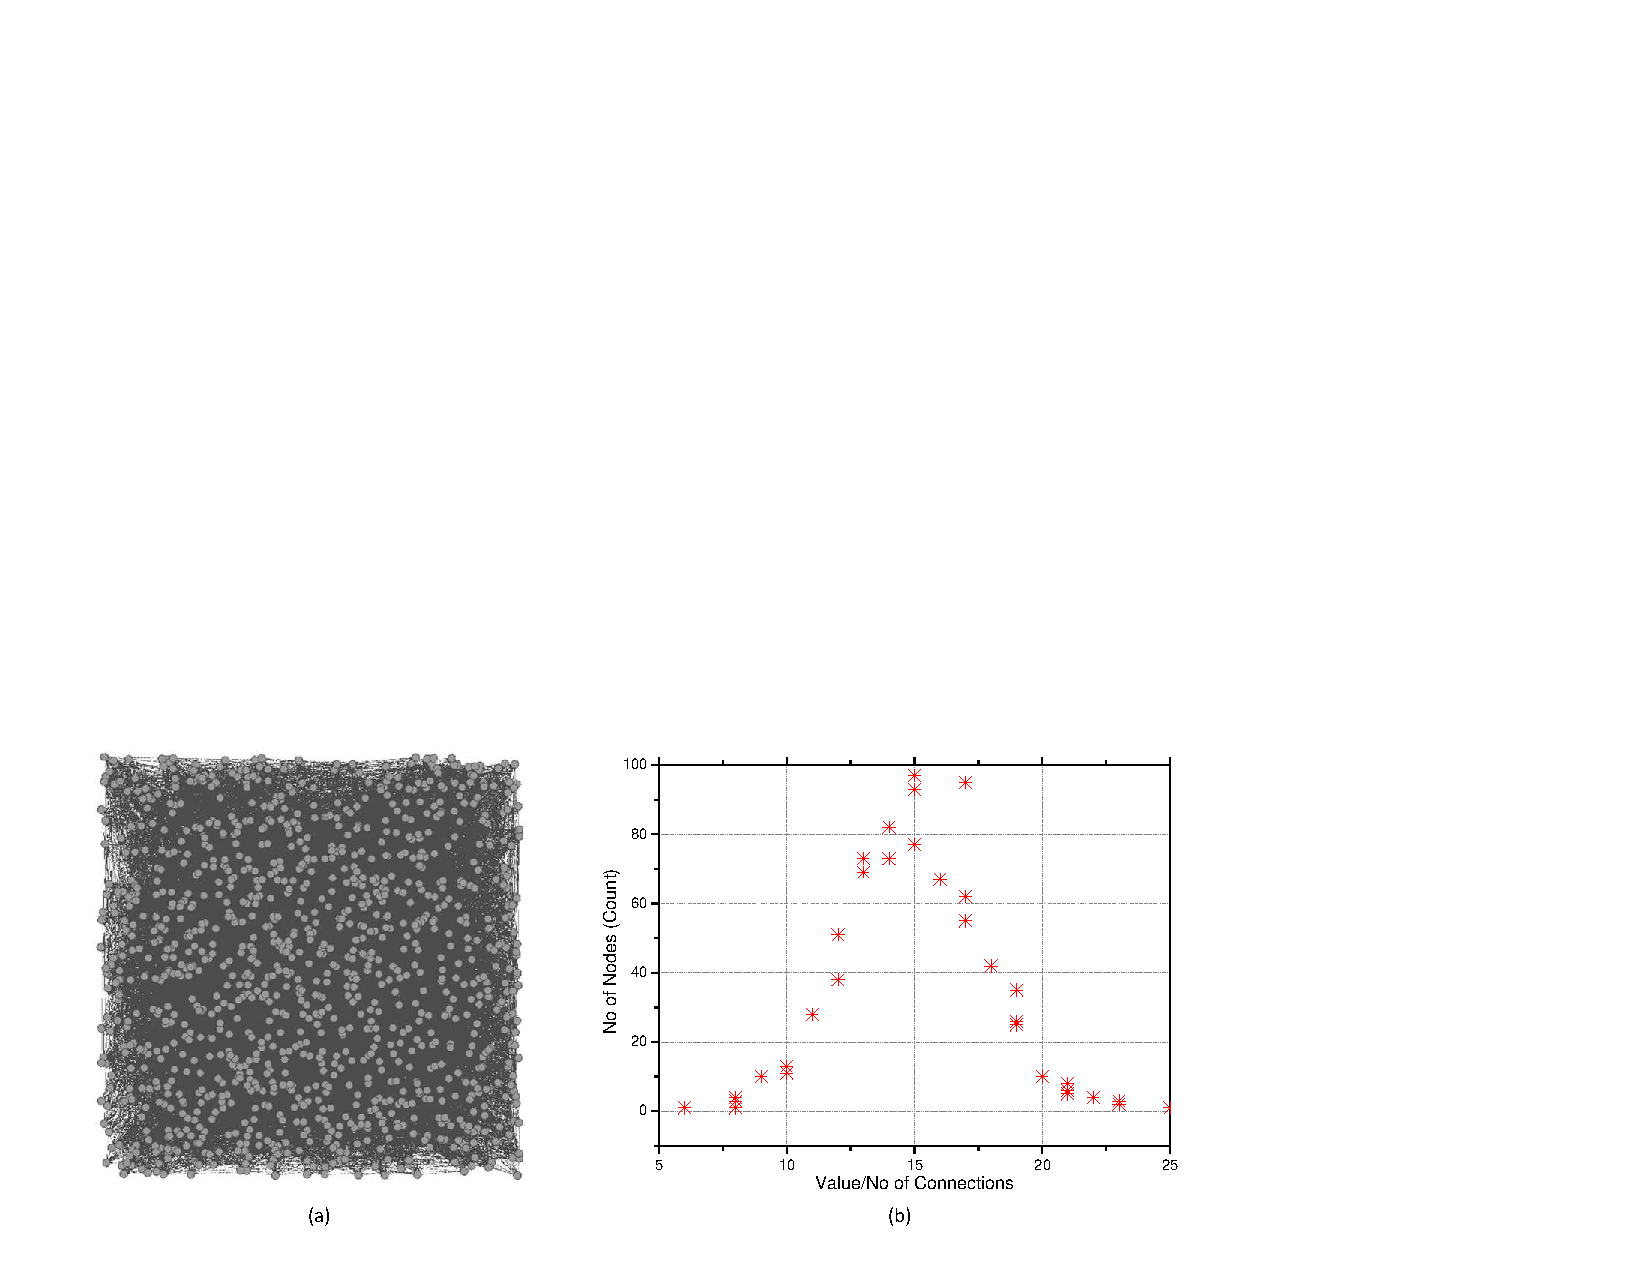
\includegraphics[width=0.9\textwidth]{Chap4-Ev-Fig0.pdf}
  \end{tabular}
  \caption{Evaluation environment (a) a social graph of 1200 nodes, with 17900 edges and average degree of 15. (b) social relationship/degree distribution showing the friendship/direct neighbor.}
\end{center}
\end{figure}

In this section, we evaluate the performance of ComPAS. There is lack of available datasets due to increasing difficulty of crawling social networks. In order to circumvent this, we created synthetic social graph to mimic the structure of social graph using RPGM. we used our own created synthetic social graph consisting of 1200 nodes, 17900 number of links/edges and average degree of 15 as depicted in Fig. 4.8 using the well-known Gephi model\footnote{Gephi is an open-source software for visualizing and analyzing large networks graphs (http://gephi.org/).}. The graph we created does not represent any specific social network in the real world, but it can be used to generate and evaluate small-scale networks. The performance of the new ComPAS data replica allocation method has been compared with the data lookup using an underlying ad-hoc replication protocol (no-replication), random replication scheme and the data replication approach W-DCG as given in~\cite{SJain2013}. In our evaluation, the range for the number of storage spaces is $G \in \{4,8,12,16\}$, and for the number of replicas, $X \in \{1,3,5,...,G-1\}$. The performance of ComPAS has been analyzed and compared with the above three protocols in terms of the metrics collected for our analysis as presented below:

\subsection{Read Cost}\label{Chap4_05_01}
\esubsection{Read Cost}

\begin{figure}[h]
\begin{center}
  \begin{tabular}{c}
  \includegraphics[width=0.95\textwidth]{Chap4-Ev-Fig1.pdf}
  \end{tabular}
  \caption{Replication efficiency in terms of read cost (no replication, random replication, W-DCG and ComPAS).}
\end{center}
\end{figure}

As seen in Fig. 4.9, without any replication, an average read cost is about nine storage space reads per user when the number of storage space is four. This cost increases slowly as more storage spaces are deployed, to a cost of about 12 when there are 16 storage spaces. The read cost improves with replication. However, the improvement of random replication is linear as more replicas are stored. W-DCG's efficiency lowers when compared to the proposed one as the numbers of replicas are increasing. Therefore, it's evident that ComPAS offers a more interesting pattern. Comparing to random replication and W-DCG in terms of replication efficiency, the proposed method is the obvious superior scheme, especially when the number of storage space is increased. Another observation from Figs. 4.9(a)-(d) is that, for each given $G$, there is a value for $X$ that maximizes the efficiency gap among the proposed one, random replication and W-DCG. Almost similar results regarding the replication efficiency of the proposed one, random replication and W-DCG are observed with all the graphs in Fig. 4.9.


\subsection{Data Accessibility and Traffic}\label{Chap4_05_02}
\esubsection{Data Accessibility and Traffic}
\begin{figure}[h]
\begin{center}
  \begin{tabular}{c}
  \includegraphics[width=0.95\textwidth]{Chap4-Ev-Fig2.pdf}
  \end{tabular}
  \caption{Effect of number of nodes on (a) data accessibility and (b) network traffic.}
\end{center}
\end{figure}

This is an important criterion for a replication protocol. Basically, data accessibility is the ratio of the number of successful access requests to the number of all access requests issued. A data replication protocol aims to increase the accessibility of data items in the network. Different than conventional static networks, in ASNETs achieving 100\% data accessibility is nearly impossible, due to mobility of nodes and changing network topology. Fig. 4.10(a) shows the variation of data accessibility with varying number of nodes in all the four replication methods including ours. As the number of nodes increases, the number of data items to be replicated in the network also increases, hence the data accessibility reduces. The graph in Fig. 4.10(a) illustrates that ComPAS provides slightly higher data accessibility than W-DCG and higher accessibility than random replication and without replication.
\begin{figure}[h]
\begin{center}
  \begin{tabular}{c}
  \includegraphics[width=0.95\textwidth]{Chap4-Ev-Fig3.pdf}
  \end{tabular}
  \caption{Relocation cost for ComPAS, W-DCG and Random replication.}
\end{center}
\end{figure}

Fig. 4.10(b) displays the variation of traffic with varying number of nodes. It is easily visible that as the number of nodes increases, the traffic for ComPAS, W-DCG and random replication also increases because every node broadcasts its properties and as the number of nodes increases groups and then social communities also increase. This results in increasing number of messages for group/community allocation and broadcasting. Traffic is zero for no replication as seen on the graph because it does not replicate data items.

\subsection{Relocation Cost}\label{Chap4_05_03}
\esubsection{Relocation Cost}
Since we want to exploit the social relationship of the network, replica relocation may happen. This property will weaken over time if replicas stay unmoved. On the other hand, if replica relocation happens too often, it results in significant overhead for the system due to communication and processing costs involved. Therefore, a desirable replica allocation method should keep the replica relocation cost as low as possible.

The relocation cost (number of replicas relocated from one storage space to another) for ComPAS, W-DCG and random replication is depicted in Fig. 4.11 for cases $G$=8 (Fig. 4.11(a)), $G$=12 (Fig. 4.11(b)) and $G$=16 (Fig. 4.11(c)). The plots shows that there exists a special value of $X$ where the relocation cost is higher. This is because, when $X$ is closer to the two extreme values (1 and $G$-1), there are too many replicas to relocate (very small $X$) and not enough flexibility for where the replicas can be relocated (very large $X$). In all the graphs (Figs. 4.11(a)-(c)), the relocation cost is small. In Fig. 4.11(a) when there are $G$=8 storage spaces, ComPAS incurs less than 0.4 replicas that need relocation. When the number of storage space $G$=16 (Fig. 4.11(c)), the relocation cost doesn't exceed 0.6 (relocated replicas). Therefore, it is obvious from the evaluation that ComPAS is highly efficient when relocation of replicas happened in the network.

\begin{figure}[h]
\begin{center}
  \begin{tabular}{c}
  \includegraphics[width=0.95\textwidth]{Chap4-Ev-Fig4.pdf}
  \end{tabular}
  \caption{The effect of relocation period on (a) Data accessibility, and (b) Traffic.}
\end{center}
\end{figure}

Next, we investigate the effect of the varied relocation period in data accessibility and traffic of W-DCG and ComPAS in Figs. 4.12(a) and (b) with the relocation period ranging from 200 to 1000. We observe from Fig. 4.12(a) that the data accessibility increases as relocation period decreases. It can be described that a shorter relocation period shows the more executions of relocation methods and, therefore, makes both replica relocation methods be able to quickly adapt to the mobility behavior of mobile nodes by frequently generating allocation units according to the network connectivity. It's also observed that ComPAS outperforms W-DCG in data accessibility. This result shows the importance of the consideration of group mobility. Therefore, the data accessibility of ComPAS is higher than that of W-DCG. In addition, the performance gain of ComPAS over W-DCG in data accessibility increases as the relocation period decreases. The reason is that each execution of ComPAS can obtain better replica allocations than that of W-DCG and, hence, a short relocation period strengthens the advantage of ComPAS over W-DCG. Fig. 4.12(b) shows the produced network traffic of ComPAS and W-DCG with varied relocation period values. We observe that the produced network traffic increases as the relocation period decreases. The reason is that with the same time interval, a shorter relocation period indicates more executions of the relocation methods and, hence, implies more exchanged messages. It is also shown that the produced network traffic of ComPAS is smaller than that of W-DCG.


\subsection{Number of Mobility Groups}\label{Chap4_05_04}
\esubsection{Number of Mobility Groups}
\begin{figure}[h]
\begin{center}
  \begin{tabular}{c}
  \includegraphics[width=0.95\textwidth]{Chap4-Ev-Fig5.pdf}
  \end{tabular}
  \caption{The effect of the number of mobility groups on (a) Data accessibility, and (b) Traffic.}
\end{center}
\end{figure}

The effects in data accessibility and traffic for both methods with varied number of mobility groups are shown in Figs. 4.13(a) and (b). The number of mobility groups is set from 1 to 100. The graph shows that the data accessibilities of ComPAS and W-DCG are equal to 100\% when the number of groups is set to one. In the case with one mobility group, the data accessibility is dependent on the initial network connectivity. In this evaluation, since the initial network topology is connected, the network topology will not be partitioned and all mobile nodes are connected throughout the simulation, thereby having complete data accessibilities for both methods. When the number of groups is set to 5, the data accessibilities are reduced to around 60\%. These results show that the data accessibilities of ComPAS and W-DCG are similar when the number of mobility groups is small. When the number of mobility groups is larger than five, the data accessibilities of both methods decrease as the number of mobility groups increases. It is because that with the same number of mobile nodes, the smaller number of mobile groups indicates that more mobile nodes are of similar moving behavior. Hence, more mobile nodes can share their storage by constructing large allocation units and, hence, increase the data accessibility.

Moreover, as shown in Fig. 4.13(a), ComPAS outperforms W-DCG especially when the number of mobility groups is large (from 10 to 50 in this simulation). The larger number of mobility groups indicates that the movement behaviors of all mobile nodes are less regular. However, the performance gain of ComPAS over W-DCG diminishes greatly when the number of mobility groups is large. Under these cases, since the network topology changes quickly and is highly likely to be partitioned into several disconnected partitions, the effect of replication diminishes significantly. Fig. 4.13(b) shows the amount of traffic produced by both methods increases as the number of mobility groups decreases. When the number of mobility groups is large, ASNET tends to be separated into many disconnected partitions since fewer mobile nodes are of similar moving behavior. Therefore, the amount of produced traffic of both methods is small since many mobile nodes disconnect with others when the ASNET is separated into several partitions.

\subsection{Efficiency of Replica Allocation Consistency}\label{Chap4_05_05}
\esubsection{Efficiency of Replica Allocation Consistency}
\begin{figure}[h]
\begin{center}
  \begin{tabular}{c}
  \includegraphics[width=0.95\textwidth]{Chap4-Ev-Fig6.pdf}
  \end{tabular}
  \caption{Consistency of ComPAS replica allocation efficiency over W-DCG and random replication for cases (a) $G$=8 storage space and (b) $G$=16 storage space.}
\end{center}
\end{figure}

To further validate the performance of our proposed replica allocation scheme, we have also performed an evaluation to measure the consistency of ComPAS's superiority to W-DCG and random replication in terms of replica allocation efficiency. We compute a measure called "after/before ratio" which is the ratio a/b where a is the improvement ratio of ComPAS over W-DCG and random replication after the relocation (relocation cost) and b is the ratio before relocation (read cost). The evaluation result is plotted in Figs. 4.14(a) and (b) for $G$=8 and $G$=16, respectively. For both cases, the ratio is consistent between 0.5 and 1. This implies that ComPAS is constantly superior to W-DCG and random replication. Besides, increase in the number of relocated replicas and storage spaces in the social graph can't have a negative impact on the effectiveness and consistency of ComPAS. Even at a higher number of nodes, replicas ($X$) and storage space ($G$) than our evaluation environment, it is evident that the efficiency and consistency will still be better for ComPAS. Finally, the results confirm the efficiency and consistency of the replica allocation method that we have proposed over W-DCG and random replication.

\section{Summary}\label{Chap4_06}
\esection{Summary}
We have introduced the importance of exploiting social properties and group mobility modeling in the replica allocation of user data for ASNETs. We have specifically proposed ComPAS, a system based on partitioning of social community combined with social relationship and a user level replication so that data availability for all users is guaranteed. The system gives a fixed number of replicas required for each user that results in an efficient replication solution. The efficiency of the proposed method is better compared to W-DCG, and by a large margin compared to random replication scheme, as shown in our evaluation and analysis. We showed that ComPAS offers significant gains in data availability, efficiency and consistency while reducing traffic and relocation cost.

\chapter{Co-Lab: Community-based Load Balancing Approach}\label{Chap5}
\echapter{Co-Lab: Community-based Load Balancing Approach}

\section{Introduction}\label{Chap5_01}
\esection{Introduction}
In socially-aware networking environments, users generate large amounts of data by exploiting capability-rich mobile devices, and prefer to share with people they have social relationships or similar interests with. However, data dissemination in this setting posses a difficult problem~\cite{YZhu2013}. As the topology is very unstable, and users appear in and disappear from the network dynamically, event producers and consumers might never connect at the same time to a given network. Therefore, data objects should be moved and replicated in the community in order for the effective delivery to interested users.  Several solutions have been proposed that consider the interest similarity of brokers and attempt to cluster brokers in such a way that the notification delay and other involved costs are minimized. For instance,  Fig. 5.1 presents an example of a dynamic solution for publish/subscribe systems. The publisher advertises an event and subsequent subscriptions are connected with the producer. Then, a consumer system relocates from broker A to broker B. After that, the topology needs to be updated in order to ensure that the event flows to broker B. Once the topology has been updated, the old subscription can be removed if there are no other subscribers at broker A.

Event-based publish/subscribe systems have been widely used in large-scale distributed applications because it allows processes to communicate asynchronously in a loosely and decoupled manner. This property gives networking systems higher modularity and re-usability as well as easier maintainability.
\begin{figure}[h]
\begin{center}
  \begin{tabular}{c}
  \includegraphics[width=0.5\textwidth]{Chap5-Fig1.pdf}
  \end{tabular}
  \caption{An example of publish/subscribe systems dynamic solution.}
\end{center}
\end{figure}
In publish/subscribe systems, loose-coupling is achieved by allowing producers to publish information in the network without knowing the identity, location, and number of subscribers. Likewise, consumers subscribe to specific information without knowing the identity, location, and number of publishers. Thus, the matching rate of both the publication and subscription determines the load of a broker~\cite{AKYCheung2010}. In turn, these factors depend on the number and nature of subscriptions that the broker serves. Therefore, load balancing is possible by offloading subscriptions from higher loaded to lesser loaded brokers. Although, load balancing has been a widely explored research topic for the past two decades, the existing offloading mechanisms do not address most of the challenges such as reducing the overall load distribution and fault-tolerance.  To the best of our knowledge, we are among the first to address load balancing and reliability by exploiting fault-tolerance techniques in event-based publish/subscribe systems.

The computing power of any distributed system can be realized by allowing its constituent computational elements, brokers or nodes, to work cooperatively so that large loads are allocated among them in a fair and effective manner. Any strategy for load distribution among these elements is called load balancing. An effective load balancing policy ensures optimal use of the system resources whereby no broker remains in an under-loaded state while any other broker is being highly utilized or overloaded. Not limited to socially-aware networks, in many today's distributed environments, the computers are linked by a delay and bandwidth is limited by communication medium that inherently inflicts tangible delays or inter-resource communications and load exchange~\cite{SDhakal2007}. To be able to fully benefit from such networking systems, resource management, data availability and reliability are key services, where issues of load balancing, partitioning and fault tolerance present a common challenge.

Recently, there has been a great effort to design and develop load balancing algorithms and fault tolerant mechanisms that are capable of improving the performance, reliability and flexibility of networking systems. Unfortunately, many practical instances of the load balancing problems have been found to be NP-complete~\cite{XZhu2011}. Hence, our work is motivated by the need for efficient algorithms which considers community formation, event dissemination, broker clustering based on interest similarity, replication, load distribution and fault-tolerance. Our main objective is to arrive at load distributions that will achieve minimum load difference between the overloaded and under-loaded brokers even during resource or link failure thereby resulting in reduced overall load distribution and a greater degree of fault-tolerance. In this chapter, we focused on designing optimal community-based load balancing and event forwarding algorithm (Co-Lab) with inspiration taken from community-based and cluster-based load balancing approaches.

The rest of this chapter is organized as follows. Related work is discussed in~\ref{Chap5_02}. \ref{Chap5_03} discusses our preliminary design. \ref{Chap5_04} discusses Co-Lab, our community-based load balancing approach. \ref{Chap5_05} presents the performance evaluation results which are analyzed and discussed, followed by a section (\ref{Chap5_06}) dedicated to conclusion and future work.

\section{Related Work}\label{Chap5_02}
\esection{Related Work}
Most of data dissemination and forwarding systems that use tree-based, DHT-based or cluster-based approaches do not provide any load balancing mechanism. Cheung and Jacobsen~\cite{AKYCheung2010} proposed a new load balancing algorithm that distributes load by offloading strategically chosen subscriptions from heavily loaded brokers to less loaded brokers. On the other hand, Zhang {\it et al.}~\cite{HZhang2008} presented the design of Shuffle, an active workload management middleware to support a scalable broker network. Shuffle offers an integral solution to manage all types of the workload in a pub/sub broker network within a single overlay topology. The need of energy efficiency is a problem concerning the constraints imposed by battery capacity and heat dissipation which are opposed by the desire of miniaturization and portability. Motivated by this observation, an energy saving and load balancing routing technique was proposed in the work of Rango and Tropea~\cite{FDeRango2009}, using a novel pheromone updating policy based on multiple performance metrics. There are a couple of existing research works that represents a first step towards the realization of a complete solution for load balancing in a cooperative, distributed environment such as kim {\it et al.}~\cite{SManfredi2013} and Manfredi {\it et al.}~\cite{HKim2012}.

Resource failures may frequently occur in socially-aware networks and have adverse effect on applications. Consequently, there is an increasing need for employing techniques to achieve fault tolerance. Therefore, fault tolerance can be provided by partitioning the network in to communities and allocating replicas of the event to those communities~\cite{Pujol2010}\cite{SGitzenis2013}\cite{MYuan2012}. Partitioning can improve availability, by ensuring that when one partition fails the remaining partitions are able to answer some of the subscriptions, and increase manageability. However, according to Curino {\it et al.}~\cite{CCurino2010}, it will not be able to predict future queries in the networks, when both data and network are changing over time. There are valuable works regarding data replication, while also guaranteeing a fair load balancing at the nodes have been tried to be addressed in our previous chapter (ComPAS) and some other existing works such as Lang {\it et al.}~\cite{WLang2010} and La {\it et al.}~\cite{CALa2012}. However, the load balancing methods they exploited are not mentioned explicitly in their work.


\section{Preliminaries}\label{Chap5_03}
\esection{Preliminaries}

\subsection{Community Partitioning}\label{Chap5_03_01}
\esubsection{Community Partitioning}

Social community can be created based on similar characteristics of individuals, including physical and social characteristics. In some cases, communities can be formed in advance; while in other cases, communities are dynamic and can only be created progressively. The specific approach for the creation of social communities depends on initiators' social goals~\cite{DZhang2011}. In this section we focus on structuring the system into communities.

We assume the network system consists of a set of brokers, $B=\{B_1,..., B_n\}$. Brokers communicate through reliable TCP links and have unique identification numbers. There are two main questions that should be answered in creating and structuring social communities. 1) How many social communities should be in the system? 2) How many brokers should be in each community? The answer for these questions directly affects the performance of the proposed load balancing approach experienced by a single broker and overall network traffic for dissemination of subscriptions and publications. Assuming subscriptions and publications of events are distributed uniformly among brokers, we want to structure communities in such a way that load distribution is uniform among brokers. We believe that this can be achieved if the sizes of communities are the same. It is straightforward to show that if the sizes of communities differ significantly, the distribution of loads among brokers will not be uniform. Fig. 5.2 displays a sample of socially-aware network structured into three communities.
\begin{figure}[t]
\begin{center}
  \begin{tabular}{c}
  \includegraphics[width=0.55\textwidth]{Chap5-Fig2.pdf}
  \end{tabular}
  \caption{Sample socially-aware network system with 6 brokers structured into 3 communities.}
\end{center}
\end{figure}

Therefore, at the beginning, the system tries to generate almost equal social communities. Assuming that the community sizes are equal, we will find the number of communities in the network system to achieve better performance through reducing overall network traffic resulted from dissemination of subscriptions and publications. In order to attain the goal, we first compute the overall network traffic in the system as follows.

Assume, there are $N$ brokers in the network system and we intend to structure them into $K$ social communities with equal sizes. The probability for a broker to have subscription matching with the advertizement or publication is $\ell(0\leq\ell\leq1)$, where $\ell$ represents the matching ratio.
\begin{equation}
TNT=AT+CT.
\end{equation}

In Equation 5.1, TNT denotes the total network traffic, AT denotes publication forwarding traffic, and CT denotes the subscription forwarding traffic. Event publication is disseminated to $K-1$ communities, where $(K-1)$ is the event dissemination traffic which results in $(K-1)$ notifications or messages. At this phase, $K$ brokers have the published notifications. Considering matching ratio $\ell$, $\ell(N-K)$ brokers out of the remaining $(N-K)$ brokers have matching subscriptions and must receive the notification. This results in an extra $\ell(N-K)$ notifications. Therefore, the $AT$ resulted from one publication is $(K-1)+\ell(N-K)$.

If we have $A$ publications/advertisements with matching ratio $\ell$ in the network system, the overall publication traffic for matching ratio $\ell$ is $A[(K-1)+\ell(N-K)]$. Assuming publications are distributed uniformly for matching ratios, the overall publication traffic for all matching ratios is computed as follows.

\begin{eqnarray}
AT&=&\int_0^1[A(K-1)+A(N-K)\ell]d\ell \nonumber\\
AT&=&A(K-1)+\frac{A}{2}(N-K).
\end{eqnarray}

When we come to the overall subscription traffic, since subscriptions are only disseminated in a community, it can be computed as follows where $C$ is the total number of subscriptions in the network system.
\begin{eqnarray}
CT&=&C\left(\frac{N}{K}-1\right)\\
TNT&=&AT+CT \nonumber\\
TNT&=&A(K-1)+\frac{A}{2}(N-K)+C\left(\frac{N}{K}-1\right).
\end{eqnarray}

We assume that the overall network traffic ($TNT$) is a function of $K$, using the number of communities in the system, we can achieve the value of $K$ that results in the minimum $TNT$ as follows.

\begin{equation}
Number~of~communities=K=\sqrt{\frac{2C}{A}N}.
\end{equation}

This equation shows that the initial number of communities in the system has a direct relation with the number of subscriptions and an indirect relation with the number of publications. By considering the amount of publications is one-fifth of the amount of subscriptions our system uses 3($\sqrt{N}$) as the initial number of communities.

\subsection{Subscription Replicating}\label{Chap5_03_02}
\esubsection{Subscription Replicating}
Most of the existing load balancing approaches including the solution by Cheung and Jacobsen~\cite{AKYCheung2010} distributes load by offloading chosen subscriptions from heavily loaded brokers to less loaded brokers. Filter-based and multicast-based are the two existing main approaches of event-based publish/subscribe systems. In the filter-based approach, subscriptions are broadcasted into the network to establish routes that direct publications to subscribers. Each publication is matched at every broker along the overlay to get forwarded towards neighbors with matching subscriptions. In the multicast-based approach, subscribers with similar interests are grouped into the same multicast set. Each publication is matched once to determine the matching multicast group(s) to which the message should be multicasted, broadcasted, or unicasted. As a result, matching and transmission of a publication message happens at most once, thus incurring minimal delivery delay. However, compared to the filter-based approach, subscribers in a multicast group may receive unwanted publications because subscribers with even slightly different interests may still be assigned to the same group~\cite{FCao2004}. Based on this fact, we propose one possible solution to this problem by integrating filter-based functionality within each multicast group.

In an event-based publish/subscribe model, a multidimensional data space is defined on $d$ attributes. An event $E$ can be represented as a set of $<a_i, v_i>$ data tuples where $v_i$ is the value this event specifies for the attribute $a_i$. A subscription can be represented as a filter $\theta$ that is a conjunction of $k$ $(k \leq d)$ predicates, and each predicate specifies a constraint on a different attribute, such as "$a_i=X$", or "$X \leq a_i \leq Y$".

To make load balance between overloaded brokers $B^o$, we propose to replicate the filters in $B^o$ to a group of under-loaded brokers $B^u$ in the community. In order to make a replica of filter, we create a cluster of brokers such that all member brokers of the cluster can maintain the same filters. Hence, a cluster G of brokers contains $N$ brokers $B_i$ with $1 \leq i \leq N$. The union of two filters (i.e. $A$ and $B$) in the cluster is the collection of filters in both $A$ and $B$. ($A \cup B={x:x \in A~or~x \in B}$)

Sets of filters cannot have duplicate elements. For example: the union of ${1,2,3}$ and ${2,4}$ is ${1,2,3,4}$. Multiple occurrences of identical elements have no effect on the cardinality of a set or its content. The same is true for the union of filters in the cluster. Denote $\theta_i$ to be the filters maintained by $B_i$ before replication. After the implementation of replication for filters on the brokers in the cluster $G$, each broker in $G$ maintains the union of filter sets as $\theta_1 \cup \theta_2 ... \cup \theta_i$.

\begin{figure}[h]
\begin{center}
  \begin{tabular}{c}
  \includegraphics[width=0.8\textwidth]{Chap5-Fig3.pdf}
  \end{tabular}
  \caption{An example of social graph based interest replication with a) no replication; b) replicating interests on $B1$ and $B2$; c) replicating interests on $B1$, $B2$, and $B3$; d) replicating interests on $B1$, $B2$, $B3$, and $B4$.}
\end{center}
\end{figure}

Let's use Fig. 5.3 to illustrate the concept of our proposed filter replication. Consider a social graph using 1 publisher, 4 brokers and 4 subscribers. The brokers $B_1$, $B_2$, $B_3$ and $B_4$ are used to connect subscribers $S_1$, $S_2$, $S_3$ and $S_4$, respectively. In the figure, we assume that all filters/interests define predicates over an attribute $year$ (movie release year). For example, $S_1$ defines a filter to be a predicate with the $year$ inside the interval [2005-2010]. That means, $S_1$ is interested in movies released between 2005 and 2010 for that particular event. Fig. 5.3(a) shows the brokers $B_1$, $B_2$, $B_3$ and $B_4$ and the maintained filter before replication. Suppose that the publishers produce a large number of advertisements having the $year$ 2010. Denote $P$ to be the number of such publication. Then, following the forwarding protocol of the friendship based social graph, all four brokers $B_1$, $B_2$, $B_3$ and $B_4$ suffer from heavy work loads to receive such $P$ publications.

To overcome the above mentioned heavy load on brokers, in Fig. 5.3(b), we initially propose to replicate the filters of $B_1$ and $B_2$. In this way, $B_1$ and $B_2$ form a cluster and maintain exactly the same generalized filters (using Union operation) $\theta_1 \cup \theta_2 = {year: [2000-2010]}$. At the same moment, brokers $B_1$ and $B_2$ builds an extra link with $S_2$ and $S_1$ respectively. Now for each of the $P$ publications, the publisher randomly chooses one of the two brokers $B_1$ and $B_2$ with equal probability of 50\%, and then forwards the publication to the chosen broker. When receiving the forwarded publication, the downstream broker finally delivers the publication to the appropriate subscribers. The brokers $B_1$ and $B_2$ then equally receive on average $P$/2 publication/advertisements, yet $B_3$ and $B_4$ still receives $P$ publications.

Next, we need to balance the loads of three brokers, in Fig. 5.3(c), we replicate the filter of $B_1$, $B_2$ and $B_3$, such that all three brokers form a cluster and maintain the same filter $\theta_1 \cup \theta_2 \cup \theta_3 = {year: [2000-2012]}$. In addition to that, the brokers build extra links with the corresponding subscribers. Now, each of the brokers $B_1$, $B_2$ and $B_3$ equally receives on average $P$/3 publications. To further balance the loads of all the brokers in the social graph, in Fig. 5.3(d), we replicate the filter of $B_1$, $B_2$, $B_3$ and $B_4$ in the same procedure as explained above. As a result of the balancing operation on all the brokers, $B_1$, $B_2$, $B_3$ and $B_4$ equally receive publications with a probability of 25\%.

Apart from the balanced loads among brokers, the uniqueness of this replication is the reduction of overall publication loads by the proposed publication algorithms given in the next subsection. It is mentioned earlier that most of the existing solutions simply offload the loads from the overloaded brokers $B^o$ to under-loaded brokers $B^u$. These solutions do not lead to the reduction of overall number of publications and can cause sudden ways of offloading filters back-and-forth across the brokers in the community. For instance, consider that the load of an overloaded broker $B^o$ is offloaded to an under-loaded broker $B^u$. After that, when there exist publications matching the filters preserved by $B^u$, the broker $B^u$ becomes overloaded and the load of $B^u$ might be moved back to $B^o$. This condition can similarly occur on the broker $B^o$, leading to a sudden way of offloading filters back and forth onto $B^o$ and $B^u$. However, in the proposed filter replication approach, there is no need to move filters back and forth onto $B^o$ and $B^u$, which eliminates the sudden ways of offloading issue.

\subsection{Event Dissemination Algorithm}\label{Chap5_03_03}
\esubsection{Event Dissemination Algorithm}
The dissemination of event $E$ is done in two phases. The first phase is dissemination among different communities (Inter-Community) where a published event is broadcasted among all communities through the publisher broker's community link ($A_{InterCom}$). In the second phase, which is dissemination of event $E$ within the community (Intra-Community), the event is matched to subscriptions in each community and is delivered to the brokers with matching subscription. Upon receiving the incoming $E$, the selected broker matches $E$ with filters including replicated filters from other clustered brokers. If the matching filters are found, the selected broker then sends $E$ to the subscribers. As shown in Algorithm 3, we propose two optional approaches to select $B_i$ among the member brokers inside community $C$. In $random~approach$, each broker in community $C$ is evenly selected with the probability of $1/C$. This approach is improved through the $greedy~method$ by selecting the broker with the smallest load inside $C$. The formal representation of the event dissemination is depicted as follows.

\begin{algorithm}
  \Begin{
    $B_A \leftarrow$ The publisher broker\;
    $A_{InterCom} \leftarrow$ The publisher broker's community link\;
    {\bf Inter-Community Phase:}\\
     \For{$B_i \in A_{InterCom}$}{
            $B_A$ sends event $E$ to $B_i$;
     }
    {\bf Intra-Community Phase:}\\
     \For{$B_i \in A_{InteCom}$}{
            $B_i$ matches event $E$ with subscription in its community\;
            \If{event $E$ matches the subscriptions}{
               i- Select a broker $B_i$ randomly\;
               ii- Select a broker $B_i$ with the smallest load\;
               Send event $E$ to the selected broker
               }
            }
  }
\caption{Pseudocode for dissemination of event $E$}
\label{alg:chap5_alg01}
\end{algorithm}

When we come to the analysis of the loads of the brokers, there is no load change for those non-clustered brokers for the filter replication operation. Therefore, we consider the loads of the clustered brokers $B_x$ inside a community C. Prior to replicating filters onto member brokers $B_x$, we took an assumption that $B_x$ maintains the filters $\theta_x$, and denote $A_{\theta_x}$ to be the set of the events matching $\theta_x$. After the replication process, suppose the filters associated with the cluster $G$ to be $\theta_G = \cup_{1 \leq i \leq G}\theta_i$, and the events matching $\theta_G$ to be $A_{\theta_G}$. The load of each broker $B_x \in G$ for the random approach on average is $A_{\theta_G}/G$. We stated above that the greedy approach achieves better result than the random approach. In order to see the load incurred using the greedy approach, let's verify it with the following explanation.

There are some different types of approximate solutions for load balancing approaches. A common one is to bound the load with an upper and lower limit~\cite{SSHTse2012}. Therefore, at the end of the greedy approach load balancing process, most of the events in any broker - the maximum load - is $\BigO{\frac{\ln A_{\theta_G}}{\ln\ln G}}$ with high probability. The original events-and-brokers process corresponds to the case where the number of cluster $G$ is 1. Surprisingly, even when $G=2$, the performance is completely different: when the process terminates, the maximum load is $\BigO{\frac{\ln\ln A_{\theta_G}}{\ln 2}}+\BigO1$ with high probability. Thus, an apparently minor change results in an exponential decrease in the maximum load. Suppose that for each publication $A$, $G \leq 2$ brokers are chosen. Each publication will be sent to the broker with the smallest load. After all the publications are sent to the selected brokers, the maximum load (upper bound) of any broker is at most $\BigO{\frac{\ln\ln A_{\theta_G}}{\ln G}} + \BigO1$ and at least (lower bound) $\BigO{\frac{\ln\ln A_{\theta_G}}{\ln G}} - \BigO1$, both with probability $1-\BigO{\frac{1}{A_{\theta_G}}}$.


\section{Inter and Intra-Community Load Balancing}\label{Chap5_04}
\esection{Inter and Intra-Community Load Balancing}
In this section we propose an optimal approach for load balancing in a community-based event dissemination system that can be employed during an event distribution process. Our load balancing strategy named Co-Lab (COmmunity-based LoAd Balancing) focuses on balancing all components on forwarding load in the community-based network system. Depending on factors such as broker's processing power, message queue size and broker's bandwidth each broker can handle certain amount of events in a time unit. We assume the maximum event messaging rate that a broker can handle is up to certain threshold. We say a broker is overloaded when the rate of event it receives, processes or forwards is higher than that certain threshold. A broker initiates load balancing process when its load reaches the threshold. The inter-community load balancing module then tries to reduce the extra load to other brokers in the system by using an offloading mechanism. Once the load among different communities is balanced then it start the intra-community load balancing mechanism as depicted in Fig. 5.4.  This phase employs the broker clustering mechanism unlike the inter-community load balancing module which applies offloading mechanism.

\begin{figure}[t]
\begin{center}
  \begin{tabular}{c}
  \includegraphics[width=0.68\textwidth]{Chap5-Fig4.pdf}
  \end{tabular}
  \caption{Co-Lab system model.}
\end{center}
\end{figure}

\subsection{Balancing Inter-Community Load}\label{Chap5_04_01}
\esubsection{Balancing Inter-Community Load}
When a broker $B_i$ is overloaded, the first step it takes to balance its load is by invoking the inter-community load balancing module. In this case, if the broker is receiving publications and subscriptions of events more than its capacity, the inter-community load balancing module decreases the broker's load by offloading the extra inter-community event dissemination load to other brokers in its community that have inter-community links/friendships with under-loaded brokers. Brokers in the same community can balance their load by invoking the similarity-based intra-community load balancing module as discussed in the following sub-section (5.4.2).

After finding the under-loaded broker, a portion of the load is sent to this broker to be processed at the intra-community level. The receiving broker treats these incoming events as the content that is received by itself and initiates a broker clustering phase. It is also possible that some of the brokers become overloaded and do not accept the incoming publications from other community. In this case, the publisher finds an under-loaded broker in its community as described above. Note that broker clustering and filter replication based on similarity are not applicable for the inter-community load balancing mechanism. The inter-community load balancing operation has two cases:
\begin{enumerate}
  \item[$\ast$]Case 1 - All the brokers in the publishers inter-community link ($A_{InterCom}$) are overloaded: the publisher broker ($B_A$) searches a broker $B_h$ in its own community which has an under-loaded inter-community link and then $B_A$ forwards the publication to $B_h$. If all the brokers ($B_i$) in $B_h$'s inter-community link are also overloaded, then $B_h$ search for a broker $B_k$ in the same community and deliver the event to $B_i$'s community through $B_k$'s inter-community link. However, if all the brokers $B_i$ in $B_h$'s inter-community link are not overloaded, then $B_h$ directly sends the event to $B_i$.
  \item[$\ast$]Case 2 - All the brokers in $A_{InterCom}$ are not overloaded (under-loaded): $B_A$ sends the event straight to $B_i$.
\end{enumerate}

\subsection{Exploiting Similarity for Intra-Community Load Balancing}\label{Chap5_04_02}
\esubsection{Exploiting Similarity for Intra-Community Load Balancing}

Our proposed filter replication solution ensures that the load of a clustered broker is in the range of [$\BigO{\frac{\ln\ln A_{\theta_G}}{\ln G}} - \BigO1$, $\BigO{\frac{\ln\ln A_{\theta_G}}{\ln G}} + \BigO1$] as shown in the previous section. It's obvious that given a number of brokers in the community, there are exponential possibilities to form clusters among the brokers. In this regard, among the exponential possibilities to make clusters of brokers, we hope that the overall load of the clusters in the community has the possibility to be lesser than the overall loads before the formation of clusters. Therefore, we initially start by exploiting similarity for clustering brokers as follows.

The minimum load among the non-clustered brokers before replication is $A_{\theta_i}$, where $\theta_i$ represents the list of filters on a particular broker $B_i$ having the load $A_{\theta_i}$. On the other hand, the maximum load inside the $G$ clustered brokers after replication is $\BigO{\frac{\ln\ln A_{\theta_G}}{\ln G}} + \BigO1$. Therefore, it is possible to conclude that clustered brokers have less load than the non-clustered brokers in the community, if the following condition satisfies.
\begin{equation}
\BigO{\frac{\ln\ln A_{\theta_G}}{\ln G}} + \BigO1 \leq A_{\theta_i}.
\end{equation}

Before we describe how to formulate and compute the similarity between filters in detail, we first give an illustration of greedy forwarding approach for checking how Equation 5.6 can be satisfied. Consider two brokers $B_1$ and $B_2$ have filters $\theta_1$ and $\theta_2$ respectively, and receive total publications of $A_{\theta_1} + A_{\theta_2} = 30$ before replication. Then, we cluster the two brokers and replicate the filters ($\theta_1 \cup \theta_2$) onto both $B_1$ and $B_2$. Our goal here is to measure the load of the clustered brokers $B_1$ and $B_2$ after the adoption of greedy forwarding approach. As shown in Table 5.1, we use five different examples for specific $\theta_1$, $\theta_2$, $A_{\theta_1}$ and $A_{\theta_2}$.

\begin{table}\fontsize{8.6}{10}\selectfont
\centering
\caption{Examples of load calculation for brokers $B_1$ and $B_2$ before and after replication}
\renewcommand{\arraystretch}{2.3}
\begin{tabular}{|c|c|c|c|c|c|c|}
\hline
\multicolumn{1}{c}{{Ex.}} & \multicolumn{1}{c}{{Similarity}} & \multicolumn{1}{c}{{$A_{\theta_1}$ [BR]}} & \multicolumn{1}{c}{{$A_{\theta_2}$ [BR]}} & \multicolumn{1}{c}{{$A_{\theta_1}$ [AR]}} & \multicolumn{1}{c}{{$A_{\theta_2}$ [AR]}} &
\multicolumn{1}{c}{{Remark}}\\
\hline
\multicolumn{1}{c}{1} & \multicolumn{1}{c}{$A_{\theta_1} \cap A_{\theta_2}=0$} & \multicolumn{1}{c}{$A_{\theta_1}=29$} & \multicolumn{1}{c}{$A_{\theta_2}=1$} & \multicolumn{1}{c}{$A_{\theta_1}=15$} & \multicolumn{1}{c}{$A_{\theta_2}=15$} & \multicolumn{1}{c}{15>1, this indicates AR incurs heavier load for $B_2$}\\
\multicolumn{1}{c}{2} & \multicolumn{1}{c}{$A_{\theta_1} \cap A_{\theta_2}=4$} & \multicolumn{1}{c}{$A_{\theta_1}=25$} & \multicolumn{1}{c}{$A_{\theta_2}=5$} & \multicolumn{1}{c}{$A_{\theta_1}=13$} & \multicolumn{1}{c}{$A_{\theta_2}=13$} & \multicolumn{1}{c}{13>5, this shows AR incurs slightly heavier load for $B_2$}\\
\multicolumn{1}{c}{3} & \multicolumn{1}{c}{$A_{\theta_1} \cap A_{\theta_2}=5$} & \multicolumn{1}{c}{$A_{\theta_1}=20$} & \multicolumn{1}{c}{$A_{\theta_2}=10$} & \multicolumn{1}{c}{$A_{\theta_1}=13$} & \multicolumn{1}{c}{$A_{\theta_2}=12$} & \multicolumn{1}{c}{12>10, AR incurs very few heavier load for $B_2$}\\
\multicolumn{1}{c}{4} & \multicolumn{1}{c}{$A_{\theta_1} \cap A_{\theta_2}=10$} & \multicolumn{1}{c}{$A_{\theta_1}=15$} & \multicolumn{1}{c}{$A_{\theta_2}=15$} & \multicolumn{1}{c}{$A_{\theta_1}=10$} & \multicolumn{1}{c}{$A_{\theta_2}=10$} & \multicolumn{1}{c}{10<15, AR leads to lighter load for both $B_1$ \& $B_2$}\\
\multicolumn{1}{c}{5} & \multicolumn{1}{c}{$A_{\theta_1} \cap A_{\theta_2}=15$} & \multicolumn{1}{c}{$A_{\theta_1}=15$} & \multicolumn{1}{c}{$A_{\theta_2}=15$} & \multicolumn{1}{c}{$A_{\theta_1}=8$} & \multicolumn{1}{c}{$A_{\theta_2}=7$} & \multicolumn{1}{c}{7<15, AR leads to balanced load for both $B_1$ \& $B_2$}\\
\hline
\multicolumn{7}{c}{(BR and AR denotes before and after replication, respectively)}\\
\end{tabular}
\end{table}

As shown in Table 5.1 that provides examples, we found out that given the similarity of filters (i.e. $\theta_1 = \theta_2$ or $\theta_1 \approx \theta_2$ in the fourth and fifth examples), the condition in Equation 5.6 satisfies. For instance, in Ex. 1 where there is no interest similarity between the events matching $\theta_1$ and $\theta_2$ ($A_{\theta_1} \cap A_{\theta_2}=0$), the replication operation incurs heavier load for $B_2$ (from one events matching this broker to 15 events). Therefore, the most valuable criterion to decide whether or not two brokers can form a cluster becomes the similarity between the corresponding filters.
\begin{equation}
Sim(B_1, B_2)=Sim(\theta_1, \theta_2)=Sim(A_{\theta_1}, A_{\theta_2}).
\end{equation}

To compute the similarity between the two filters ($Sim(\theta_1, \theta_2)$), we choose to consider the publications that match $\theta_1 \cap \theta_2$ and $\theta_1 \cup \theta_2$. Based on this logic, we measure the similarity between two brokers $B_1$ and $B_2$ as follows.
\begin{equation}
Sim(\theta_1, \theta_2)=\frac{A_{\theta_1} \cap A_{\theta_2}}{A_{\theta_1} \cup A_{\theta_2}}.
\end{equation}

The two formulas above (i.e. Equations 5.7 and 5.8) cover both the filters and publications matching the filters. In the remaining part of this section, we would like to cluster brokers having high similarity within the community based on the defined similarity metrics as shown in Algorithm 4.

\begin{algorithm}
  \Begin{
     Create and initiate a temporary storage $\chi$, and a list $\nu$ to contain set of clusters of brokers\;
     \For{pair of brokers $B_i$ and $B_j$}{
         store $Sim(B_i, B_j)$ together with $[B_i, B_j]$ to $\chi$;
     }
     \While {$\chi \neq$ empty}{
         get $[B_i, B_j]$ in descending order of $Sim(B_i, B_j)$ (highest similarity first)\;
         \If {both $B_i$ and $B_j$ are already clustered}{
            No action is needed;
         }
        \If{$B_i$ or $B_j$ (i.e. $B_j$) is already in cluster $G_1$}{
            \If {adding $B_i$ to $G_1$ satisfies Equation 5.6}{
                add $B_i$ to $G_1$;}
            \Else
                {start a new cluster $G_2$, add $B_i$ to it, and add $G_2$ to $\nu$;}
            }
        \Else (//both $B_i$ and $B_j$ are not clustered)
                {start a new cluster $G_2$, add both $B_1$ and $B_2$ to it, and add $G_2$ to $\nu$;
        }
        Temporary storage $\chi$ is empty
     }
     \For{$G \in \nu$}{
        replicate filters and create links among member brokers in $G$;
     }
}
\caption{Pseudocode of broker clustering}
\label{alg:chap5_alg02}
\end{algorithm}

\section{Evaluation}\label{Chap5_05}
\esection{Evaluation}
In this section, we evaluate the performance of our proposed load balancing scheme Co-Lab, by comparing it with the method (we call it Offloading) proposed by Cheung and Jacobse~\cite{AKYCheung2010}, Shuffle~\cite{HZhang2008}, and event dissemination algorithm with no particular load balancing approach (we name it as No Load Balancing). One of the main challenges we faced in evaluating our approach is the lack of real world application datasets. However, it is possible to create and generate a topology that mimics the structure of social graph for publish/subscribe network systems. Therefore, we used our own social graph applied in chapter~\ref{Chap4} (ComPAS). The generated graph has 1200 nodes, 17900 number of links/edges with average degree of 15. Communities are structured based on the method presented in sub-section~\ref{Chap5_03_01}. We then randomly chose nodes in the community as brokers, publishers and subscribers.

The matching ratio $\ell$ (ranging from 0 to 100\%) was used to generate filters and publications. Using wide variety of $\ell$ in our evaluation, the results can be interpreted for both Zipf and unform distributions. The parameter range for number of brokers, publishers and subscribers is 0-500, 0-50 and 0-250, respectively. By varying the number of these parameters we conducted the evaluation. As a default, we used 500 broker, 50 publisher and 250 subscriber nodes. The normal distribution is represented by 0.5$\ell$, where the probability of subscriptions is almost equal for all events. High (>50$\ell$) and low (<50$\ell$) implies Zipf distribution where some events are very popular and have many subscribers while other events are very selective and a small number of brokers have subscriptions for these events. The performance of Co-Lab has been analyzed and compared with Offloading, Shuffle, and No Load Balancing in terms of the metrics collected for our analysis as mentioned below.

\subsection{Event Dissemination Load Distribution}\label{Chap5_05_01}
\esubsection{Event Dissemination Load Distribution}
\begin{figure}[t]
\begin{center}
  \begin{tabular}{c}
  \includegraphics[width=0.95\textwidth]{Chap5-Ev-Fig1a.pdf}
  \end{tabular}
  \caption{Load distribution of event dissemination for Community-based, Cluster-based, DHT-based and Tree-based approaches based on (a) 0.25$\ell$, (b) 0.5$\ell$, (c) 0.75$\ell$.}
\end{center}
\end{figure}

As depicted in Figs. 5.5(a)-(c), we first compare our approach (community-based load balancing) with three other common load balancing approaches, tree-based, DHT-based, and cluster-based. The evaluation is based on the number of events that is managed by a broker in one time unit and the publications and subscriptions are uniformly distributed among brokers. Figs. 5.5(a)-(c) presents the dissemination of load distribution for three different matching ratios ($\ell$=0.25, $\ell$=0.5 and $\ell$=0.75). Tree-based approach performs the worst in case of load distribution. In all the denoted matching ratios, there are several brokers with very high amounts of load, while there are brokers with very small amounts of load. This can be reasonable based on the tree structure of the broker where any publication from one side that has matching subscription on the other side of the tree must pass through the brokers. These brokers are processing almost all the publications which results in high dissemination load. On the other hand, brokers in the edge of the tree do not participate in publication dissemination very often which results in very small load. The DHT-based system performs somewhat better than the tree-based one, and cluster-based performs better than both tree-based and DHT-based. However, in all cases our community-based load balancing method, disseminates the load more consistently and uniformly among brokers and circumvent highly overloaded brokers.

\begin{figure}[t]
\begin{center}
  \begin{tabular}{c}
  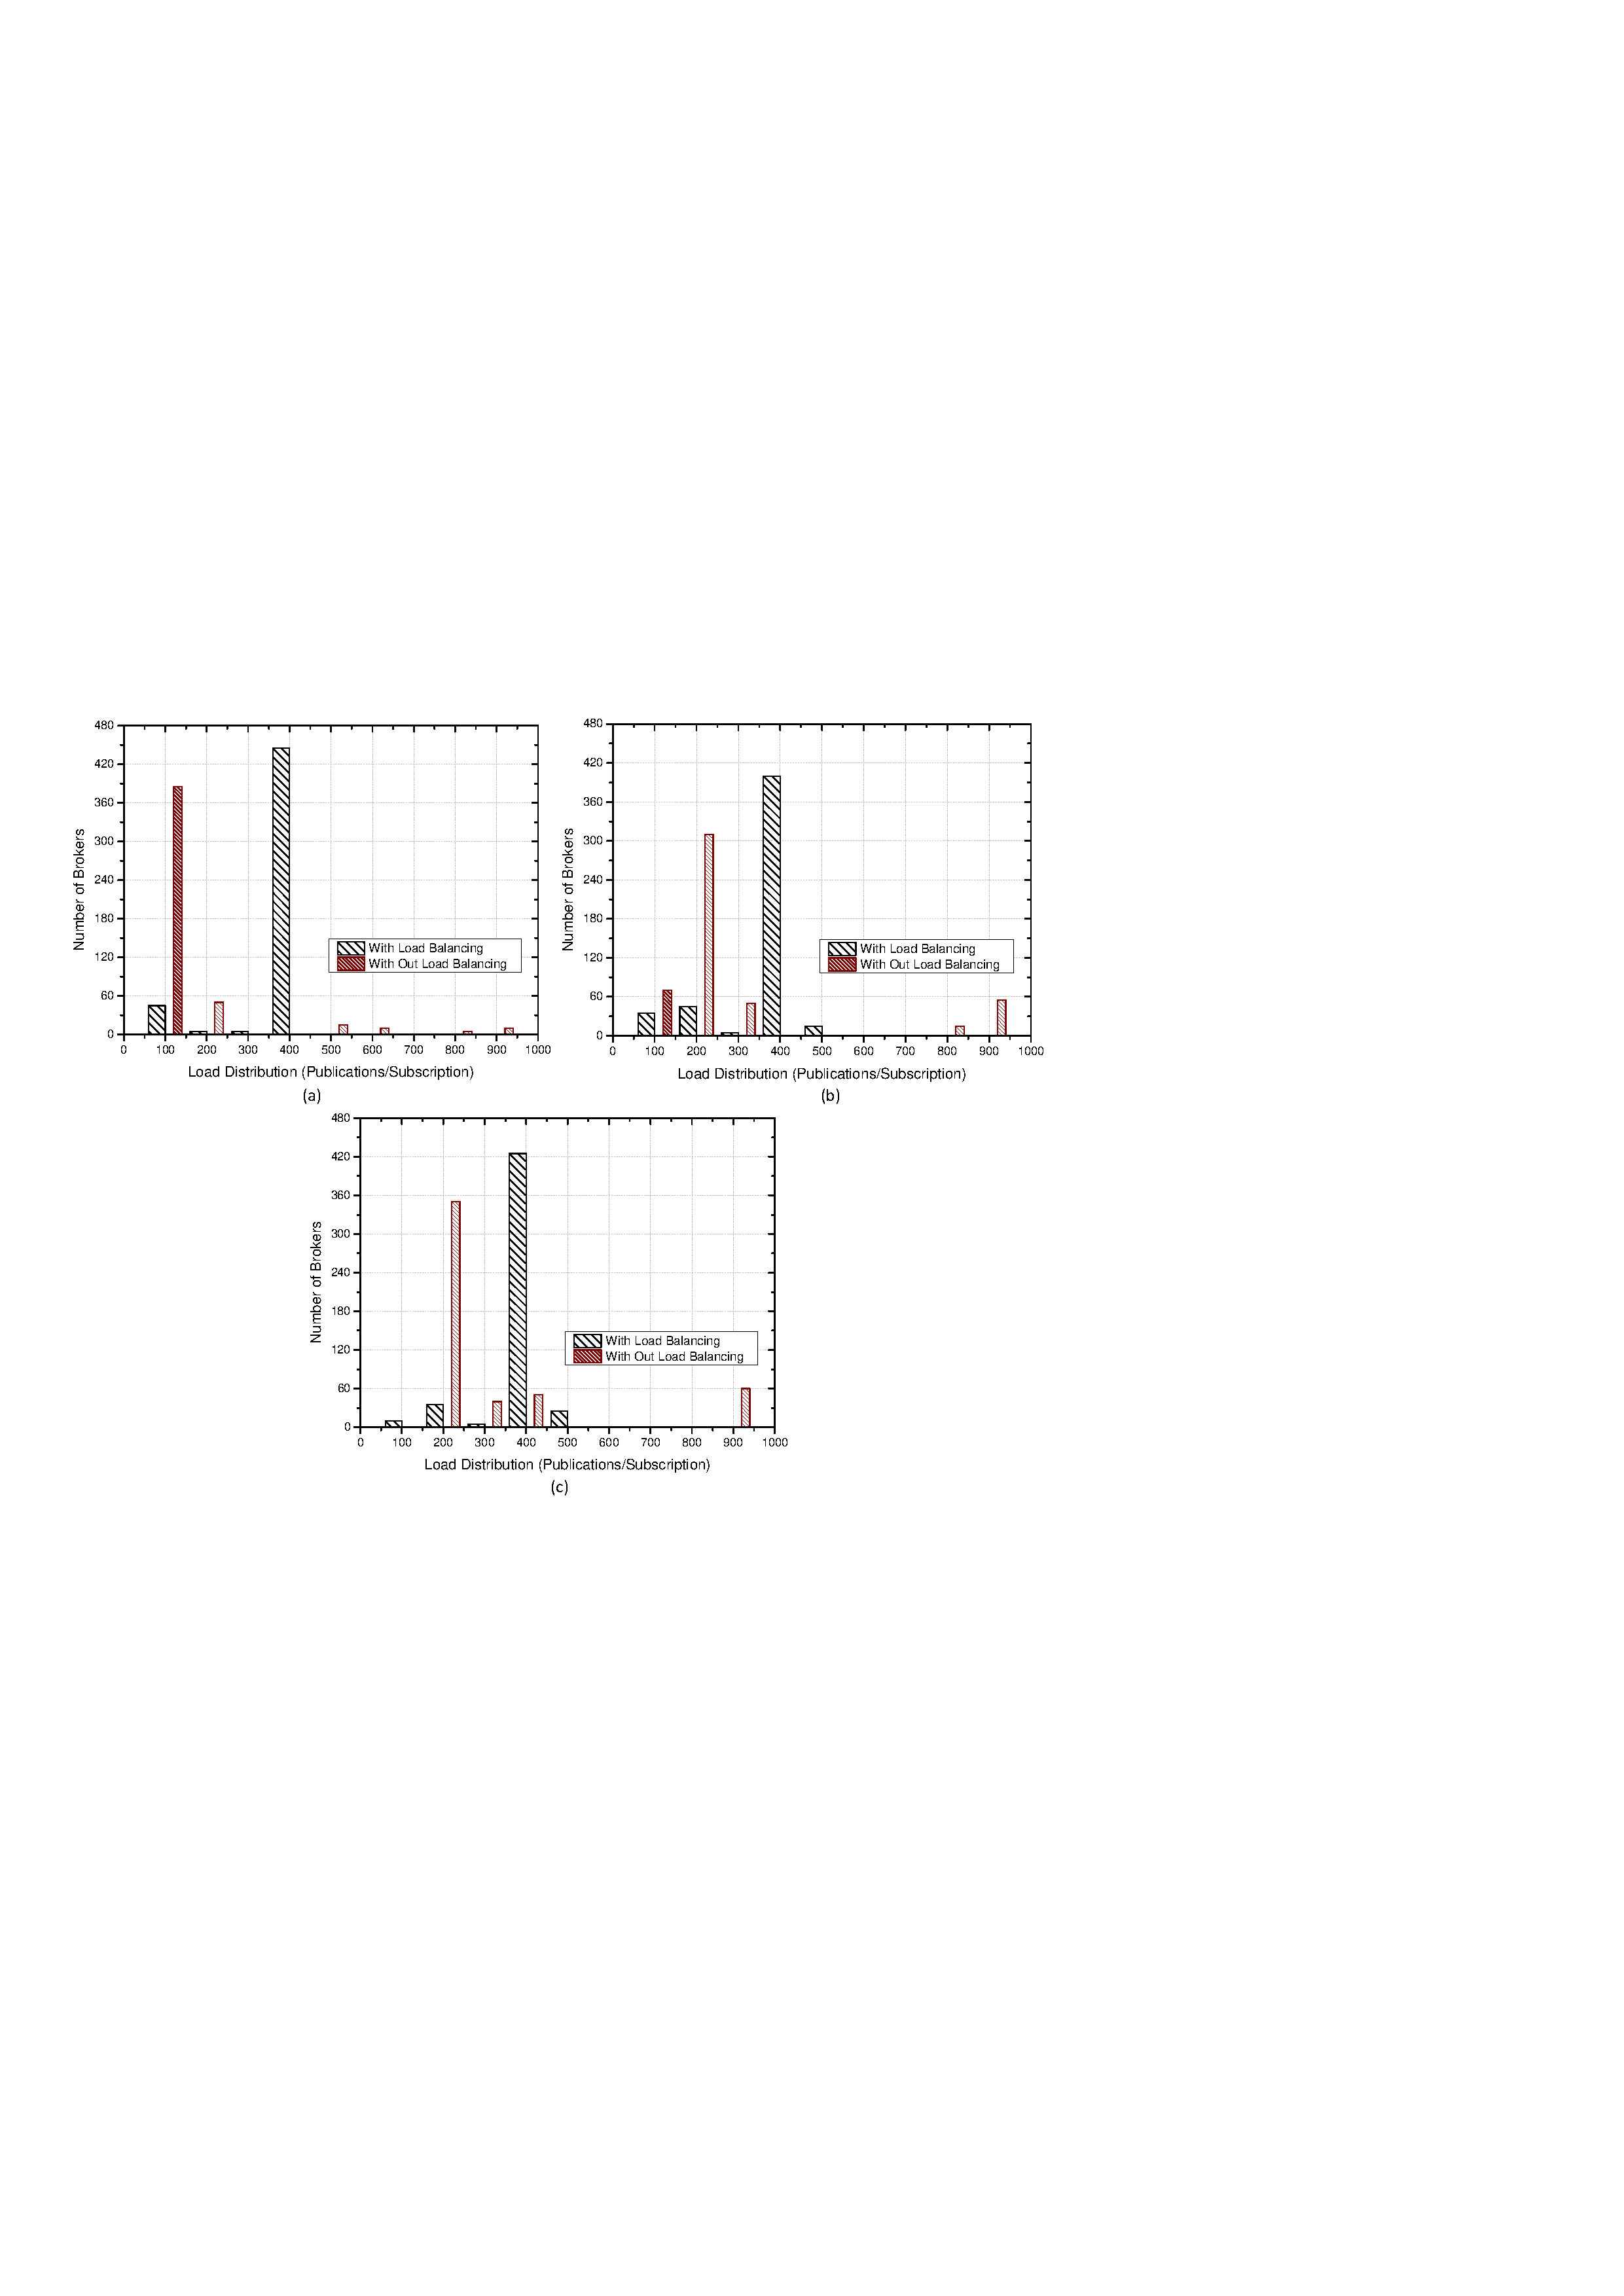
\includegraphics[width=0.95\textwidth]{Chap5-Ev-Fig1b.pdf}
  \end{tabular}
  \caption{Community-based event dissemination with and without load balancing mechanism based on (a) 0.25$\ell$, (b) 0.5$\ell$, (c) 0.75$\ell$.}
\end{center}
\end{figure}

In Figs. 5.6(a)-(c), we present the evaluation of the proposed community-based technique with and without load balancing in order to show the significance of the load balancing algorithm. Our method is compared with the other using three different matching ratios, 25\% ($\ell$=0.25), 50\% ($\ell$=0.5) and 75\% ($\ell$=0.75). The plots clearly show that when the publication distribution among brokers follows Zipf distribution (for $\ell$=0.25 and $\ell$=0.75), the community-based approach without load balancing results in irregular or uneven distribution of dissemination load. This is because of concentration of dissemination load on a small portion of inter-community in the network which results in higher dissemination load on the brokers while the other brokers in the other communities remain under-loaded. Contrarily, in community-based event dissemination with load balancing, brokers at the inter-community link with higher load offloads some of the load to brokers in the other community link with smaller load which results in more uniform distribution of load among brokers. As seen in Fig. 5.6(a), regarding community-based with load balancing, almost 90\% of brokers have a load in range [300, 400] and there is no broker with higher load. However, the same plot with no load balancing technique shows that the load distribution is very skewed and more than 70\% of brokers have a load in range [0, 100] while around 15\% of brokers have a load higher than 500. The same results are obtained for $\ell$=0.5 and $\ell$=0.75 which validates our load balancing method in efficiently balancing the load among brokers and preventing broker overloading as much as possible.

\subsection{Overall Load}\label{Chap5_05_02}
\esubsection{Overall Load}
To evaluate the overall load, we specify and amount the overall publications received by all brokers in the community. As depicted in Fig. 5.7(a), as the number of brokers increases it incur heavier overall loads for all the load balancing approaches (Co-Lab, Offloading, Shuffle and No Load Balancing). The logic behind this is that, when more brokers are employed on the generated social graph, the subscription clients are more distinctly distributed to the brokers. Therefore, publications are forwarded towards more number of brokers until the publications are received by the last subscribers in the community. The total number of publications are then increased. However, it is noted from the figure that, the average number of event publication per broker becomes smaller. For instance, when the number of brokers grows from 250 to 500, the overall load of our proposed approach, Offloading, Shuffle, and No Load Balancing are increased by 20\%, 22.23\%, 31.67\%, and 30.26\% respectively, while the average publication per broker is decreased by 37.5\%, 35.71\%, 26.83\%, and 28.3\%.
\begin{figure}[t]
\begin{center}
  \begin{tabular}{c}
  \includegraphics[width=0.95\textwidth]{Chap5-Ev-Fig2.pdf}
  \end{tabular}
  \caption{Overall workloads of all brokers in the communities based on the effect of (a) brokers, (b) publishers, and (c) subscribers.}
\end{center}
\end{figure}

Fig. 5.7(b) displays, when the number of publishers increases the system generates more publications, resulting in heavier loads for all the approaches including ours. However, Co-Lab has fewer overall loads than the other three methods. For instance, when the numbers of publishers are at the maximum, which is 50, compared with Offloading, Shuffle, and No Load Balancing, our proposed method achieves 48.98\%, 58.33\%, and 64.29\% reductions of the overall load respectively. Furthermore, the increase in number of subscribers results in heavier overall load for all the approaches; Co-Lab, Offloading, Shuffle, and No Load Balancing. The fact is that, when we balance the number of publishers and the overall generated events, the publications have to be forwarded to more subscribers with a consistently large number of publications, which results in heavier loads as depicted in Fig. 5.7(c). For instance, when the numbers of subscribers are at the maximum, which is 250, compared with Offloading, Shuffle, and No Load Balancing, our proposed method achieves 52\%, 63.02\%, and 70\% reductions of the overall load respectively.

\subsection{Load Distribution}\label{Chap5_05_03}
\esubsection{Load Distribution}
We use a variable $\Omega$ [1, 5] of distribution to measure the load distribution of every broker as displayed in Figs. 5.8(a)-(c). When the $\Omega$ value is higher, there is an even distribution of load among brokers.  As plotted in Fig. 5.8(a), as the numbers of broker increases from 0 to 500, the value of $\Omega$ also increases for all four methods including Co-Lab resulting in a better balanced loads among brokers in the community. When there is large number of brokers, there exist more brokers in the system satisfying the condition of Equation 5.6 to reduce the loads of those overloaded brokers and transfer it to the under-loaded brokers. As a result it achieves better balanced loads of brokers for Co-Lab, Offloading, Shuffle, and No Load Balancing methods.
\begin{figure}[t]
\begin{center}
  \begin{tabular}{c}
  \includegraphics[width=0.95\textwidth]{Chap5-Ev-Fig3.pdf}
  \end{tabular}
  \caption{Load distribution measurement of every broker in their respective communities as influenced by (a) brokers, (b) publishers, and (c) subscribers.}
\end{center}
\end{figure}
\begin{figure}[t]
\begin{center}
  \begin{tabular}{c}
  \includegraphics[width=0.95\textwidth]{Chap5-Ev-Fig4.pdf}
  \end{tabular}
  \caption{The effect of varying time on (a) load distribution, (b) overall loads, and (c) overhead of the load balancing methods.}
\end{center}
\end{figure}

In Fig. 5.8(b), we evaluate the effect of number of publishers on the performance of Co-Lab, Offloading, Shuffle, and No Load Balancing. When the number of publishers increases, $\Omega$ value also increases resulting in better balanced load among brokers. Furthermore, as displayed on the figure Co-Lab achieves higher $\Omega$ value than the other three methods. For instance, when the number of publishers reaches the maximum, the $\Omega$ values of Co-Lab, Offloading, Shuffle, and No Load Balancing are 3.3, 3, 2.25, and 1.2 respectively. Moreover, when we vary the number of subscribers from 0 to 250, the $\Omega$ values of all the presented methods grow as shown in Fig. 5.8(c). The reason behind this result is that, more subscribers' results in more subscriptions to the brokers.

\subsection{Load Balancing and Overhead}\label{Chap5_05_04}
\esubsection{Load Balancing and Overhead}

As shown in Figs. 5.9(a)-(c), we investigate the effect of load balancing vary with time on load distribution, overall loads and overhead. We found out that the value of $\Omega$ for all the methods become increasing from the beginning to 2000s and keep on almost the same $\Omega$ value after the moment of 2000 seconds as depicted in Fig. 5.9(a). This implies that the loads are becoming better balanced. Next, we evaluate the overall load distribution by varying the time. As plotted in Fig. 5.9(b), the overall load of all the methods gradually decreases as the time increases. At time 2000s, the overall number of publications of Co-Lab, Offloading, and Shuffle becomes 63.48, 103.54, and 193.46 respectively. Hence, it is obvious to validate that, at the moment of 1 hour Co-Lab can minimize the overall loads resulting to 37.04\% and 65.66\% reductions than Offloading and Shuffle respectively.

In addition to the above performance evaluations, we also measure the overhead of the load balancing methods implicitly incurred by the links created among brokers maintaining the filters and subscribers. The overhead of all the methods increased at the beginning and then decreases at time 2000s. After that, the overhead of Co-Lab, Offloading and Shuffle keeps on the close range of [42, 52], [33, 42], and [22, 32], respectively as displayed in Fig. 5.9(c). This result shows that our proposed approach incurs a higher overhead than the other two methods while achieving the advantage of balancing loads and reducing overall loads of brokers. The reason for higher overhead incurred by Co-Lab is the creation of more links between brokers and subscribers in the cluster after filter replication. Notwithstanding  this drawback, we have validated that the proposed Co-Lab outperforms other methods on the whole.

\section{Summary}\label{Chap5_06}
\esection{Summary}
We have introduced the importance of integrating filter-based and multicast-based publish/subscribe systems for designing a community-based load balancing method. We have specifically proposed Co-Lab; a community-based load balancing method combined with fault-tolerance techniques that minimizes overloaded brokers by distributing the event publication load among brokers. Our proposed technique includes an inter-community phase that employs an offloading mechanism to reduce the overall load distribution among communities. We also proposed an intra-community load balancing phase that can distribute and balance the load among brokers in a community. We implemented an interest based similarity filter replication while clustering the brokers in the community. This resulted in balanced loads as well as a maximized reliability.

We validated the effectiveness of the proposed approach through extensive evaluations. Our performance evaluation results show that load balancing mechanism implementing a community-based approach is significantly better than the existing tree-based, DHT-based and cluster-based systems. We have also shown that Co-Lab can efficiently distributes the load among brokers and reduces the overall load distribution in the system better than Offloading and Shuffle techniques.

\chapter{BoDMaS: Bio-Inspired Algorithm to Detect and Counteract Selfishness}\label{Chap6}
\echapter{BoDMaS: Bio-Inspired Algorithm to Detect and Counteract Selfishness}

\section{Introduction}\label{Chap6_01}
\esection{Introduction}
Emerging socially-aware networks that leverage social behaviors of participating users to improve networking throughput is gradually dominating wireless communication towards replacing traditional wireless networks. Among various socially-aware networks, ASNETs are gaining momentous ground due to their unique characteristics, particularly low resource consumption cost, mobility support, and infrastructure-less settings. Such features are often observed in biological processes that inspire inventing and designing novel cooperative architectural concepts~\cite{SBalasubramaniam2011}. ASNETs are proliferating as the common communication platform in broadly important areas such as pervasive conference/meetings and health-care, remote environmental monitoring and public safety, and ubiquitous urban data acquisition and national defense.

In socially-aware networking environments, users generate large amounts of data by exploiting capability-rich mobile devices which are willing to share their capabilities with users through social relationships, social ties or greater similar interests. However, successful adoption of ASNET services (e.g., data dissemination and replication), is inhibited in the absence of motivation/incentive for participating users who collaborate and share their resources. Cooperation among users is crucial to the survival of the network, as it forms the basis for key network services. If  users (selfish users) refuse to collaborate in delivering the network services, end-to-end connection may not be possible leading to network performance degradation. Existing solutions assume that users are willing to collaborate with others \cite{MEirinaki2014}. However, users in practice are selfish with varied degrees of selfishness (from non-selfish to fully-selfish) depending on the strength of their social-tie with the underlying network, especially when there is no cooperating motivation/incentive \cite{QLi2010}. Selfish users are unwilling to spend their precious resources for operations that do not directly benefit them~\cite{KGopalakrishnan2009}. For example, they may be willing to collaborate with socially-tied users (e.g., friends, co-workers, room-mates), but not others. Fig. 6.1 shows an example of a selfish user who inhibits efficient data forwarding in an exemplary scenario. The sender user $S$ has two route choices ($S\rightarrow A\rightarrow B \rightarrow R$ and $S\rightarrow A \rightarrow C\rightarrow D\rightarrow R$) to forward data to the user $R$ at the receiver side; one is 3-hop and another 4-hop far from receiver. Though efficient networking demands data transmission through lower-hop route (3-hop in this example), the selfish user $B$ located in middle of 3-hop route inhibiting data transmission via this route. Hence, transmission must be carried out via longer route over 4 hops leading to higher communication overhead \cite{SAbolfazli2014}. Therefore, it is essential to detect selfish users and isolate them to limit their negative behavioral impact on the network performance.
\begin{figure}[t]
\begin{center}
  \begin{tabular}{c}
  \includegraphics[width=0.5\textwidth]{Chap6-Fig1.pdf}
  \end{tabular}
  \caption{An example demonstrating user selfishness in forwarding data from source to destination.}
\end{center}
\end{figure}

Although a variety of solutions aim to address the problem of detecting and isolating misbehaving users in wireless networks~\cite{JChoi2011}, most existing works have focused on addressing selfishness by employing approaches such as reputation \& incentive based~\cite{MTRefaei2010}, trust-based~\cite{UVenkanna2013}, ACK-based~\cite{NKang2010}, game-theory~\cite{KAkkarajitsakul2013} or quorum-based~\cite{EMannes2012} mechanisms to incentivize and motivate users to collaborate in services for others. In spite of significant findings in the detection and isolation of users' selfishness, there are still numerous issues that limit their applicability~\cite{SDjahel2011}. Firstly, social behaviors of participating nodes are neglected in design and development of existing algorithms and hence makes them inefficient to be directly applied to ASNETs to deal with selfishness. Secondly, a huge overhead is induced from sharing reputation information amongst the users, additional acknowledgment packets dissemination, and decision ambiguity that arises if the requested user refuses to return an acknowledgment. Thirdly, cooperative users might be indirectly punished due to their location in the network. Fourthly, network might be flooded by when a user sends the same data several times to the same receiver. Lastly, existing bio-inspired solutions (such as~\cite{EMannes2012}) in this field of research consider only quorum systems without social behavior consideration such as social ties.

ASNETs lack a centralized controlling and monitoring terminal, thus, making it a challenging task to  effectively detect and isolate such misbehaving nodes from the network. Selfishness is a non-cooperative act of misbehavior, which is notably different from malicious behavior. It is noteworthy that our focus in this chapter is only on selfishness and thus we ignore malicious behaviors. To overcome the above limitations of existing algorithms, we design a bio-inspired algorithm named BoDMaS aiming to detect and counteract selfishness in ASNETs where high cooperation is highly desirable. We develop our work taking inspiration from a biological mechanism resident in bacteria (quorum sensing) and social community systems. Our initial results are extremely encouraging, indicating that the choice of social behavior is critical and that novel techniques can be successfully imported from biologically inspired models.

In this chapter, we are mainly focusing on user's behavior with respect to data replication operations (i.e., query/update) at the top of the data management model. Under this focus, each user can be classified as either cooperative (well-behaving) or selfish (misbehaving). This model may also apply to malicious users indirectly to some extent when it comes to timeout manipulations. However, malicious behavior is not to be under-estimated and shall undoubtedly be considered in our future work. Other classes of reliability model (trust and adversary) are also outside the scope of this chapter. The remainder of this chapter is structured as follows. \ref{Chap6_02} reviews related works in the literature. \ref{Chap6_03} presents an overview of the system model and assumptions. \ref{Chap6_04} provides the detailed design architecture and briefly describes the functions of each BoDMaS component. Section~\ref{Chap6_05} demonstrates the effectiveness of our proposed system and discusses the results. The last section formalizes the conclusion from the work conducted.

\section{Related Work}\label{Chap6_02}
\esection{Related Work}
There are several research works that have applied the above mentioned approaches. Gera {\it et al.}~\cite{PGera2011} proposed an opinion-based cooperative trust model in the presence of malicious nodes. With respect to the behavior observed, each node determines the trustworthiness of the other nodes. Their trust model exploits information sharing among nodes to accelerate the convergence of trust establishment procedures, and is further robust against the propagation of false trust information by malicious nodes. However, continuous information sharing overhead is degrading native resources of wireless nodes in the network. The authors in~\cite{DHales2005} focus on the problem of maintaining significant levels of cooperation in peer-to-peer networks. Their algorithm is adapted from novel "tag" models of cooperation that do not rely on explicit reciprocity, reputation or trust approaches. Another line of work by Li and Cao~\cite{QLi2012} uses contact records based on which the next contacted node can detect if the node has dropped any packet in order to develop a distributed scheme to detect selfishness in DTNs. The same authors of~\cite{QLi2012} have published a scheme named SSAR (Social Selfishness Aware Routing) ~\cite{QLi2010}, which considers both users' willingness to forward and their contact opportunity to select a forwarding node, resulting in a better forwarding strategy than those based solely on contact. However, in non of these works, focus is given to the selfish attitude of nodes and researchers are trying to motivate cooperation among nodes.

McCoy {\it et al.}~\cite{DMcCoy2007} presented MIND, a reputation-based authentication protocol for identifying and handling misbehaving and malicious users in the neighborhood. In this protocol, each user conducts a continuous follow-up over its neighbor user's forwarding behavior by comparing the incoming and outgoing data of its neighbor. However, this can cause a higher detection rate for false positives. Furthermore, when a user queries its neighbors and if the reply is invalid or fails to reply, the user decides that a neighbor has failed without giving any reason for the failure. In addition to the reputation-based mechanisms, there are some proposals on enforcing collaboration for wireless ad-hoc networks (i.e.,~\cite{NJiang2007}), addressing the problem of resilience in the network with the presence of misbehaving users (i.e.,~\cite{HJLeBlanc2013}) and blacklisting misbehaving users while maintaining the privacy in the network (i.e.,~\cite{PPTsang2011}).

LeBlanc {\it et al.}~\cite{HJLeBlanc2013} showed that users' connection or neighborhood is no longer adequate for the assurance of resilient consensus when the users use their own inbuilt nature that only require each user to know its own neighborhood. However, the results in their proposal apply to directed graphs and consider undirected graphs as an exceptional case. In addition to that, they categorize misbehaving users as a restricted type of Byzantine user in which every user is required to send similar message to all of its neighbors which causes the users to consume high energy.  On the other hand, Nymble~\cite{PPTsang2011} has been proposed with the aim of permitting anonymous blacklisting of misbehaving users. This proposal tries to reinvent the common practice of address banning, without actually telling a user's address. However, this protocol exposed to some sensitive security and trust issues reducing from the usage of trusted third parties that can simply work together to disrupt a user's secrecy.

From Komali {\it et al.}'s~\cite{RSKomali2008} and Pelechrinis {\it et al.}'s~\cite{KPelechrinis2012} perspective, it is difficult to justify the cooperative theory because nodes are either competing for network resources or conserving their own limited resources. Therefore, they proposed an algorithm called DIA($\delta$-Improvement Algorithm) in which each node makes some decrements in its power level if the change improves its operation. However, their performance evaluation shows that there might be a fundamental conflict between an efficient and fair allocation. It shows that it is important to integrate load balancing and fairness mechanisms to misbehavior detection mechanisms, to predict how much the user is willing to offer his resources to strangers under a probabilistic framework and assign other utilities mechanism. However, these algorithms are unable to fulfill unique requirements of ASNETs.

Data management, particularly data availability is one of the most crucial tasks in ASNET environments. Replication is one of the prominent techniques for ensuring the accessibility of data among partitioned communities. Data replication is a technique of creating and managing replica. Replica is a data item that is stored redundantly at multiple communities. In chapter~\ref{Chap4}, we proposed ComPAS which detailed the means of allocating replicas in different communities in order to increase data availability. However, one of the assumptions in designing the system model is that all the participating users are cooperative in every aspect, such as forwarding read queries and update operations which is not the reality in ASNETs. In order to address challenges emerging from misbehaving users in replication operations for MANETs, Mannes {\it et al.}~\cite{EMannes2012} proposed $QS^2$ by incorporating bio-inspired mechanisms into quorum systems. Quorum systems are powerful mathematical tools to reason about distributed implementations of shared objects including read/write operations~\cite{JLuo2003}. In particular, quorum systems have been used for reasoning in implementations that tolerate misbehavior and are optimally resilient to process failures. More sophisticated forms of quorum systems have been introduced to cope with different failures and these require larger intersections among quorums, eventually leading to an increased overhead.

Drawing from the analogy with existing quorum systems as communities, we believe that applying biologically inspired mechanisms~\cite{SBalasubramaniam2011} in this regard will help to reduce the limitations of existing algorithms. This has also been proved in the work from our lab~\cite{FXia2014} related to data forwarding for socially-aware networks. To the best of our knowledge, BoDMas is the first work to consider social willingness in designing a bio-inspired algorithm to detect and neutralize the impacts of selfish users within dynamically changing network conditions of ASNETs.

\section{Models and Assumptions}\label{Chap6_03}
\esection{Models and Assumptions}
In this section, we first present the overall model of a simplified ASNET system illustrated in Fig. 6.2 and explain inter-layers interactions and functionality of its major components. Subsequently, we discuss matching analogy between bacteria operation and ASNET functionality. Network model (including social graph and user mobility components), data management model (consisting of replication and load balancing components), and reliability model (comprising attack, trust, and adversary components) are described. The successful operation of ASNETs entirely depends on the cooperation among sub-models and components. For scalability and resilience reasons the current system model needs to be redesigned.

\begin{figure}[t]
\begin{center}
  \begin{tabular}{c}
  \includegraphics[width=0.55\textwidth]{Chap6-Fig2.pdf}
  \end{tabular}
  \caption{Simplified ASNET Middleware System Model.}
\end{center}
\end{figure}

\subsection{Network Model}\label{Chap6_03_01}
\esubsection{Network Model}
Network in ASNET is modeled using social graph and user mobility. Social networks exhibit the small world phenomenon that node encounters are sufficient to build a connected relationship graph~\cite{FXia2013}. Such a graph is an abstract graph where vertices represent individual people and edges describe social ties between individuals. Through the use of a social graph, a variety of social metrics (e.g. social relationship, communality, centrality, and similarity) can be easily calculated. Therefore, it is crucial to obtain social graphs for social-based data management design approaches like ASNETs.

We model the social community network as a bidirectional, weighted communication that is symmetrical at every link between users. It means that if a user $Y$ is able to receive a message from user $X$ at time $t$ then user $X$ can also receive a message from user $Y$ at time $t$. As in other studies~\cite{QLi2010}, \cite{KGopalakrishnan2009}, this assumption is often valid using selected wireless MAC layer protocols (i.e. IEEE 802.11) requires bidirectional communication for reliable transmission. The network is composed of a vertex set $G$ of all $n$ users/nodes identified by $\{d_0, d_1 ... d_{n-1}, d_n\}$, and a set of edges, $E$, to be the social links between users. Every user $d_i \in G$ has a unique address or identification and the same processor and energy capacity. The weight of edge $XY$ is $X$'s willingness to forward query/update packets for $Y$. The weight of edge $XY$ and that of $YX$ may be different. In ASNETs, users have limited bandwidth and computational capability. Furthermore, users are assumed to rely on intermediate users to route packets since they may not reach directly due to their coverage area~\cite{HBLiaqat2014}.
\begin{figure}[h]
\begin{center}
  \begin{tabular}{c}
  \includegraphics[width=0.55\textwidth]{Chap6-Fig3.pdf}
  \end{tabular}
  \caption{Illustration of user mobility within an ASNET of 32 users. There are four communities (denoted using the gray dotted lines) and 32 mobile users(denoted using circles), where some users are selfish (represented by the red dashed circles) and some are roaming outside a community (moving directions are represented using arrows).}
\end{center}
\end{figure}

User mobility is another component in modeling ASNET networks. Users move according to the group movement pattern in a surrounded area. Community partitions in the network can occur when the network between the communities fail simultaneously due to movement of users or scarce resources. Group mobility refers to the scenario where several mobile users tend to move together. The system tries to solve the problem of selfishness in replication operations by exploring group mobility. The underlying group mobility model is assumed to be RPGM as used in chapter~\ref{Chap4} of this dissertation. In our system, each mobile user first exchanges its motion behavior with its neighbor based on the social relationship in the community. Mobile users may collaborate and, hence, move as a group instead of independently. RPGM is a better choice to model this kind of team collaboration behavior. As shown in Fig. 6.3, all users are divided into several mobility groups and all mobile users within the same mobility group are of similar moving behavior~\cite{AMAhmed2014}.

\subsection{Data Management Model}\label{Chap6_03_02}
\esubsection{Data Management Model}
In ASNETs, replication helps to avoid data losses in case of an unpredictable group mobility that causes community partition and also aids in reducing the number of hops when a data is transmitted. This work employs ComPAS (Chapter \ref{Chap4}) as the data management (replication) model. Note that, other schemes could be applied, nevertheless, ComPAS was chosen because it can significantly improve ASNETs performance by exploiting social relationship while replicating in the community to achieve better efficiency and consistency which makes it more appropriate. Further, it can also reduce the query delay, since users can get the data replicas from some nearby communities. By replicating, data availability can be improved because there are multiple replicas in the network and the probability of finding one copy of the data is high~\cite{ADerhab2009}. {\it Replica} is a data item that is stored redundantly at multiple communities. We define data replication as a technique of creating and managing duplicate versions of data items. Users comprise of performing two types of operations: {\it query} and {\it update}.

Simply, ComPAS is a system based on partitioning of social community combined with social relationship and a user level replication so that data availability for all users is guaranteed. The system gives a fixed number of replicas required for each user that results in an efficient replication solution. It is based on a perception that if we need to place a replica copy for a user $i$ somewhere, the most desirable location should be the primary storage place of most neighbors of $i$; this way, most neighbors will benefit from this replica when they issue a read query. Furthermore, it aims to find an efficient and consistent way to store $X$ replicas for each user's data in the storage space at $Y$ communities $(X < Y)$ and it choose the value of $X$ depending on the replication budget of the system and its desired availability. For detailed illustration of ComPAS's operation, refer to Chapter \ref{Chap4}.

\subsection{Reliability Model}\label{Chap6_03_03}
\esubsection{Reliability Model}
Reliability in ASNET can be verified from a different perspective. Our way of understanding categorizes it as attack, trust and adversary components.  As mentioned in the previous sections, among the components our focus is only on the {\it attack component (selfishness)}. Selfish users work in the network for their own benefit. They simply do not cooperate with other users in data transmission process to conserve their own energy, or give priority to their own interest. These selfish users disturb the performance of ASNET to a great extent. {\it Trust} is a critical determinant of sharing information and developing new relationships in a network~\cite{YNajaflou}. Although trust is not our target and it is not essential to our proposed scheme, we assume the source of data is anonymous to intermediate users. Other technical aspects related to trust such as authentication is out of the scope of this dissertation. Malicious attacks (i.e. modifying or injecting malicious data in the replication system) and free-riding behaviors are grouped in {\it adversary component} and not our focus.

\subsection{Ad-hoc Social Network and Bacteria Analogy Matching}\label{Chap6_03_04}
\esubsection{Ad-hoc Social Network and Bacteria Analogy Matching}
In biological systems, two main entities can be observed~\cite{JLFernandez-Marquez2013}, namely (1) the organism that collaborates in the biological process (e.g., virus, ants, bees, fish, and bacteria) and (2) the environment (i.e., communities in ASNET). Among these, bacteria have complex social properties resulted from their communication abilities that govern their colony. These social behaviors enable the bacteria to evolve through various fluctuating environmental situations by utilizing cooperative and non-cooperative behaviors~\cite{MHasan2014}. They use quorum sensing to coordinate actions that cannot be carried out by a single bacterium. As individual and limited functionalities, their adjustment to the environment is very limited and therefore they rely on mobility. Quorum sensing can be defined as a decentralized coordination process which allows bacteria to estimate the density of their population and regulate their behavior accordingly by focusing on production and detection of chemical products called Acyl-Homoserine Lactone Autoinducers (AHL-Ai). Each bacterium is similar to a mobile node that extracts information from the environment, interprets the information, develops common knowledge and learns from past experiences~\cite{AEinolghozati2012}. Our proposed algorithm, considers social willingness as a social behavior and the characteristics observed in bacteria as a biological mechanism. AHL-Ai (hereafter $A_i$ for the sake of simplicity and brevity) acts as a signaling chemical gradient to detect and determine the amount of bacteria in the environment, allowing them to develop a collaborative behavior for the whole group, depending on the amount of bacteria engaged. The social behavior existence in both the community and bacteria makes a dynamic and autonomous solution, inspiring the proposed algorithm.
\begin{figure}[t]
\begin{center}
  \begin{tabular}{c}
  \includegraphics[width=0.65\textwidth]{Chap6-Fig4.pdf}
  \end{tabular}
  \caption{BoDMaS Architecture.}
\end{center}
\end{figure}

\section{Detailed Design}\label{Chap6_04}
\esection{Detailed Design}
Throughout this section, we present the overall architecture of our BoDMaS proposal and describe how BoDMaS fits into the typical ASNET system. We also describe functional interaction among BoDMaS components and provide algorithm pseudocode. We also discuss our model verification approach.

\subsection{BoDMaS Architecture}\label{Chap6_04_01}
\esubsection{BoDMaS Architecture}
BoDMaS aims to detect user's selfishness and counteract it to maintain the reliability of replicated data. Using three major components of behavior assessment, user classification, and user selection \& reaction, our proposal detects selfish users and takes actions against the involvement of selfish users in replication operations (i.e., query and update). The behavior assessment is executed by comparing social willingness level and observation of $A_i$ represented by the amount of replica updates, queries, and forwards issued by users. Fig. 6.4 present an illustrative view of our proposal consisting three basic components, namely: {\it behavior assessment}, {\it user classification} and {\it user selection \& reaction}.

Fig. 6.5 depicts interaction sequence among these major BoDMaS components. The behavior assessment component adopts and monitors social willingness level for intermediate users. Based on the score $A_i$ from the assessment, the next component evaluates the users in the process. The user classification component uses the score to compare it with the threshold ($Thr$) and identifies users with selfish behavior. Finally, the user selection \& reaction component selects cooperative users in order to perform data update and query operations, and takes action against selfishness by notifying other users. The remaining part of this section describes the details of each BoDMaS component.
\begin{figure}[t]
\begin{center}
  \begin{tabular}{c}
  \includegraphics[width=0.6\textwidth]{Chap6-Fig5.pdf}
  \end{tabular}
  \caption{Functional interaction among BoDMaS components.}
\end{center}
\end{figure}

\subsection{Behavior Assessment}\label{Chap6_04_02}
\esubsection{Behavior Assessment}
To select an appropriate user for the operation, BoDMaS considers both users' willingness and $A_i$ counts. In our context, a social willingness means an interpersonal social tie between users that falls into the strong or weak range. A selfish user may demonstrate different behavior (cooperative) for users with strong social relationship. That is, the user is willing to provide better service to those with stronger ties than those with weaker ties, especially when there are resource constraints~\cite{QLi2010}. The work of Li {\it et al.}~\cite{HLi2012} presented three ways of assigning social willingness level: Uniform Distribution of Social Ties (UST), Clustered Distribution of Social Ties 1 (CST1) and Clustered Distribution of Social Ties 2 (CST2). Among these, we use UST that uniformly assigns random values between [0, 1] as willingness level ($\rho_{id}$) for the friendship between users.

The social willingness level between each pair of users $i$ and $d$ is characterized by a rational number $\rho_{id} \in$ [0, 1], where $\rho_{id}$ = 1 is strongest and $\rho_{id}$ = 0 means no willingness at all. Based on this value, the source user chooses the direct neighbor that has strong social tie as an input to the next step. High willingness level does not indicate that the user is not selfish, because there are cases in which the selected neighbor can hold or ignore the received data without doing the job (here is one of the importance of $A_i$ counter). To count replica forward operations $A_{i(f)}$, each user $i$ has $A_i$ counter linked with each neighbor having a social relationship in the community. The counting is conducted based on the communication between users, and occurs when a user receives replica query or update requests. Requesters attach their ID to the packet such that the behavior assessment component can use it to increment $A_{i(f)}$ counter for every user in the line (from source to destination).

\subsection{User Classification}\label{Chap6_04_03}
\esubsection{User Classification}
This component implements users' scores, assigned by the behavior assessment component (and possibly the sequence of operations that led to each score), to identify selfish users in the network. A common approach is to compare the user's score to the $Thr$ expected from a cooperative user. In order to get the correct $Thr$, the expected rate of forwards $Er_f$ according to the behavior of replication has to be estimated. This rate is calculated within a given period of time and used to set $A_{i(f)}$ threshold. A user that has $A_i$ count lower than this limit is classified as selfish.

\subsection{User Selection \& Reaction}\label{Chap6_04_04}
\esubsection{User Selection \& Reaction}
Finally, this component selects the cooperative users based on the score to perform the data operations. It also informs other users to avoid approaching selfish users. For example, in the case of update operations on replica, suppose that $Er_{f(min)}$ threshold is 3 forwards per second, a user whose score is greater than or equal to 3 is considered cooperative. Users with lower scores are classified as selfish. Algorithm \ref{alg:chap6_alg01} presents detailed BoDMaS operations.
\begin{algorithm}
\Begin{
    $\rho_{id} \leftarrow$ Social willingness level ($\rho_{id} \in$ [0, 1])\;
    $A_i \leftarrow$ Autoinducers count\;
    $A_{i(f)} \leftarrow$ Autoinducers count for replica forward\;
    $Thr \leftarrow$ Score expected from a cooperative user\;
    $Er_{f(min)} \leftarrow$ Minimum query and update forwards at time $t$\;
    {\bf Behavior assessment:}\\
     \For{all direct neighboring users}{
            compares $\rho_{id}$; where 1 is strongest and 0 is none;
            increment $A_{i(f)}$ counter for every user in the line (from source to destination);
     }
    {\bf User classification:}\\
            \For{all users' scores collected}{
            compare a user's score to a $Thr$\;
            \If{User $A_i$ count < $Thr$ limit}{
               classify the user as selfish\;
               $Er_{f(min)}$ value is identified\;
               }
    }
    {\bf User selection \& reaction:}\\
            take action against users according to their behavior\;
            \If{User score $\geq$ $Er_{f(min)}$}{
               user is considered cooperative\;
               perform data operations using cooperative users and notify other users about selfish users\;
               }
}
\caption{Pseudocode for BoDMaS}
\label{alg:chap6_alg01}
\end{algorithm}

To correctly verify the entire model, it is essential to calculate some values such as True Detection Rate ($TDR$) and False Detection Rate ($FDR$). Thus, we employ a set $M(b,r)$, containing all interactions of selfish users and a set $C(b,r)$ representing interactions of cooperative users in both query and update operations where $b$ represents the user class (either selfish or cooperative) after the detection result by BoDMaS and $r$ is the real class of that user. $TDR$ represents the amount of detected selfish users and it is calculated using Equation \ref{eq1}.
\begin{equation}\label{eq1}
TDR = \frac{\sum K_i}{|M|}  \hspace{1cm} \forall \hspace{0.4cm}i \in M,
\end{equation}
where $K_i$ = 1 if $b_i$ = $r_i$ and $K_i$ = 0 if $b_i \neq r_i$.

$FDR$ is of two types: False Negative ($FN$) and False Positive ($FP$). $FN$ detects the selfish users mistakenly classified as cooperative users. This is calculated using Equation \ref{eq2} with all the same $TDR$ assumptions.
\begin{equation}\label{eq2}
FN = \frac{\sum K_i}{|M|}\hspace{1cm} \forall \hspace{0.4cm}i \in M,
\end{equation}
where $K_i$ = 1 if $b_i \neq r_i$ and $K_i$ = 0 if $b_i$ = $r_i$. $FP$ measures the amount of cooperative users classified as selfish as shown in Equation \ref{eq3}, where $C$ denotes all the cooperative interactions. It's modeled as $C(b, r)$ where $r$ = 1 and 0 represents a selfish and cooperative users, respectively.
\begin{equation}\label{eq3}
FP = \frac{\sum K_i}{|C|}\hspace{1cm}\forall \hspace{0.4cm}i \in C,
\end{equation}
where $K_i$ = 1 if $b_i$ = $r_i$ and $K_i$ = 0 if $b_i \neq r_i$. The next section presents performance and efficiency evaluation results.

\section{Demonstration of Effectiveness}\label{Chap6_05}
\esection{Demonstration of Effectiveness}
\begin{table}
\centering
\caption{Simulation Parameters}
\renewcommand{\arraystretch}{1.5}
\begin{tabular}{|l|l|l|l|l|}
\hline
\multicolumn{1}{c}{Parameter} & \multicolumn{1}{c}{Value}\\
\hline
\multicolumn{1}{c}{Number of users} & \multicolumn{1}{c}{32}\\
\multicolumn{1}{c}{Number of communities} & \multicolumn{1}{c}{4} \\
\multicolumn{1}{c}{Defined area } & \multicolumn{1}{c}{400m X 400m} \\
\multicolumn{1}{c}{Users/community} & \multicolumn{1}{c}{$\approx$ 8}\\
\multicolumn{1}{c}{Number of simulations} & \multicolumn{1}{c}{10 trials}\\
\multicolumn{1}{c}{Simulation time} & \multicolumn{1}{c}{10 mins}\\
\multicolumn{1}{c}{User movement} & \multicolumn{1}{c}{RPGM}\\
\multicolumn{1}{c}{Maximum speed} & \multicolumn{1}{c}{2 - 20 m/s (variable)}\\
\multicolumn{1}{c}{Pause time} & \multicolumn{1}{c}{10s - 100s (variable)}\\
\multicolumn{1}{c}{Expected updating rate} & \multicolumn{1}{c}{$\lambda$ = 80}\\
\multicolumn{1}{c}{Expected querying rate} & \multicolumn{1}{c}{$\lambda$ = 24}\\
\multicolumn{1}{c}{Forward threshold} & \multicolumn{1}{c}{$Er_{f(min)}$ = 0.2 forwards per second}\\
\multicolumn{1}{c}{Number of selfish users} & \multicolumn{1}{c}{$N_{selfish}$ = 2, 4, 8 and 16 users}\\
\multicolumn{1}{c}{Confidence interval} & \multicolumn{1}{c}{95\%}\\
\hline
\end{tabular}
\end{table}
In this section, we present performance and efficiency evaluation of BoDMaS based on accessibility degree, detection rates, and network load balance. Results obtained by the evaluation of ComPAS integrating BoDMAS (represented by ComPAS$\uplus$BoDMaS) is compared to ComPAS without BoDMaS within the same scenarios. The scheme is analysed considering the presence of selfish users in ComPAS operations. The network is composed of 32 users within 4 communities, and users move according to RPGM into an area of 400$m^2$. The maximum speed range is 2-20 m/s with a varying pause time of 10s-100s. The expected updating and querying rates are $\lambda$=80 and $\lambda$=24, respectively. The forwarding threshold $Er_{f(min)}$ is 0.2 forwards per second. This scenario intends to represent an academic conference environment of mobile users that consists of different participants such as authors, organizers, speakers moving towards some common locations in the conference hall. The information shared concern about participants interest, like topics of presentations or key notes at multiple session rooms. Table 6.1 summarizes the detailed evaluation parameters we use for simulation to demonstrate the effectiveness of our algorithm.

\subsection{Accessibility Degree}\label{Chap6_05_01}
\esubsection{Accessibility Degree}
\begin{figure}[t]
\begin{center}
  \begin{tabular}{c}
  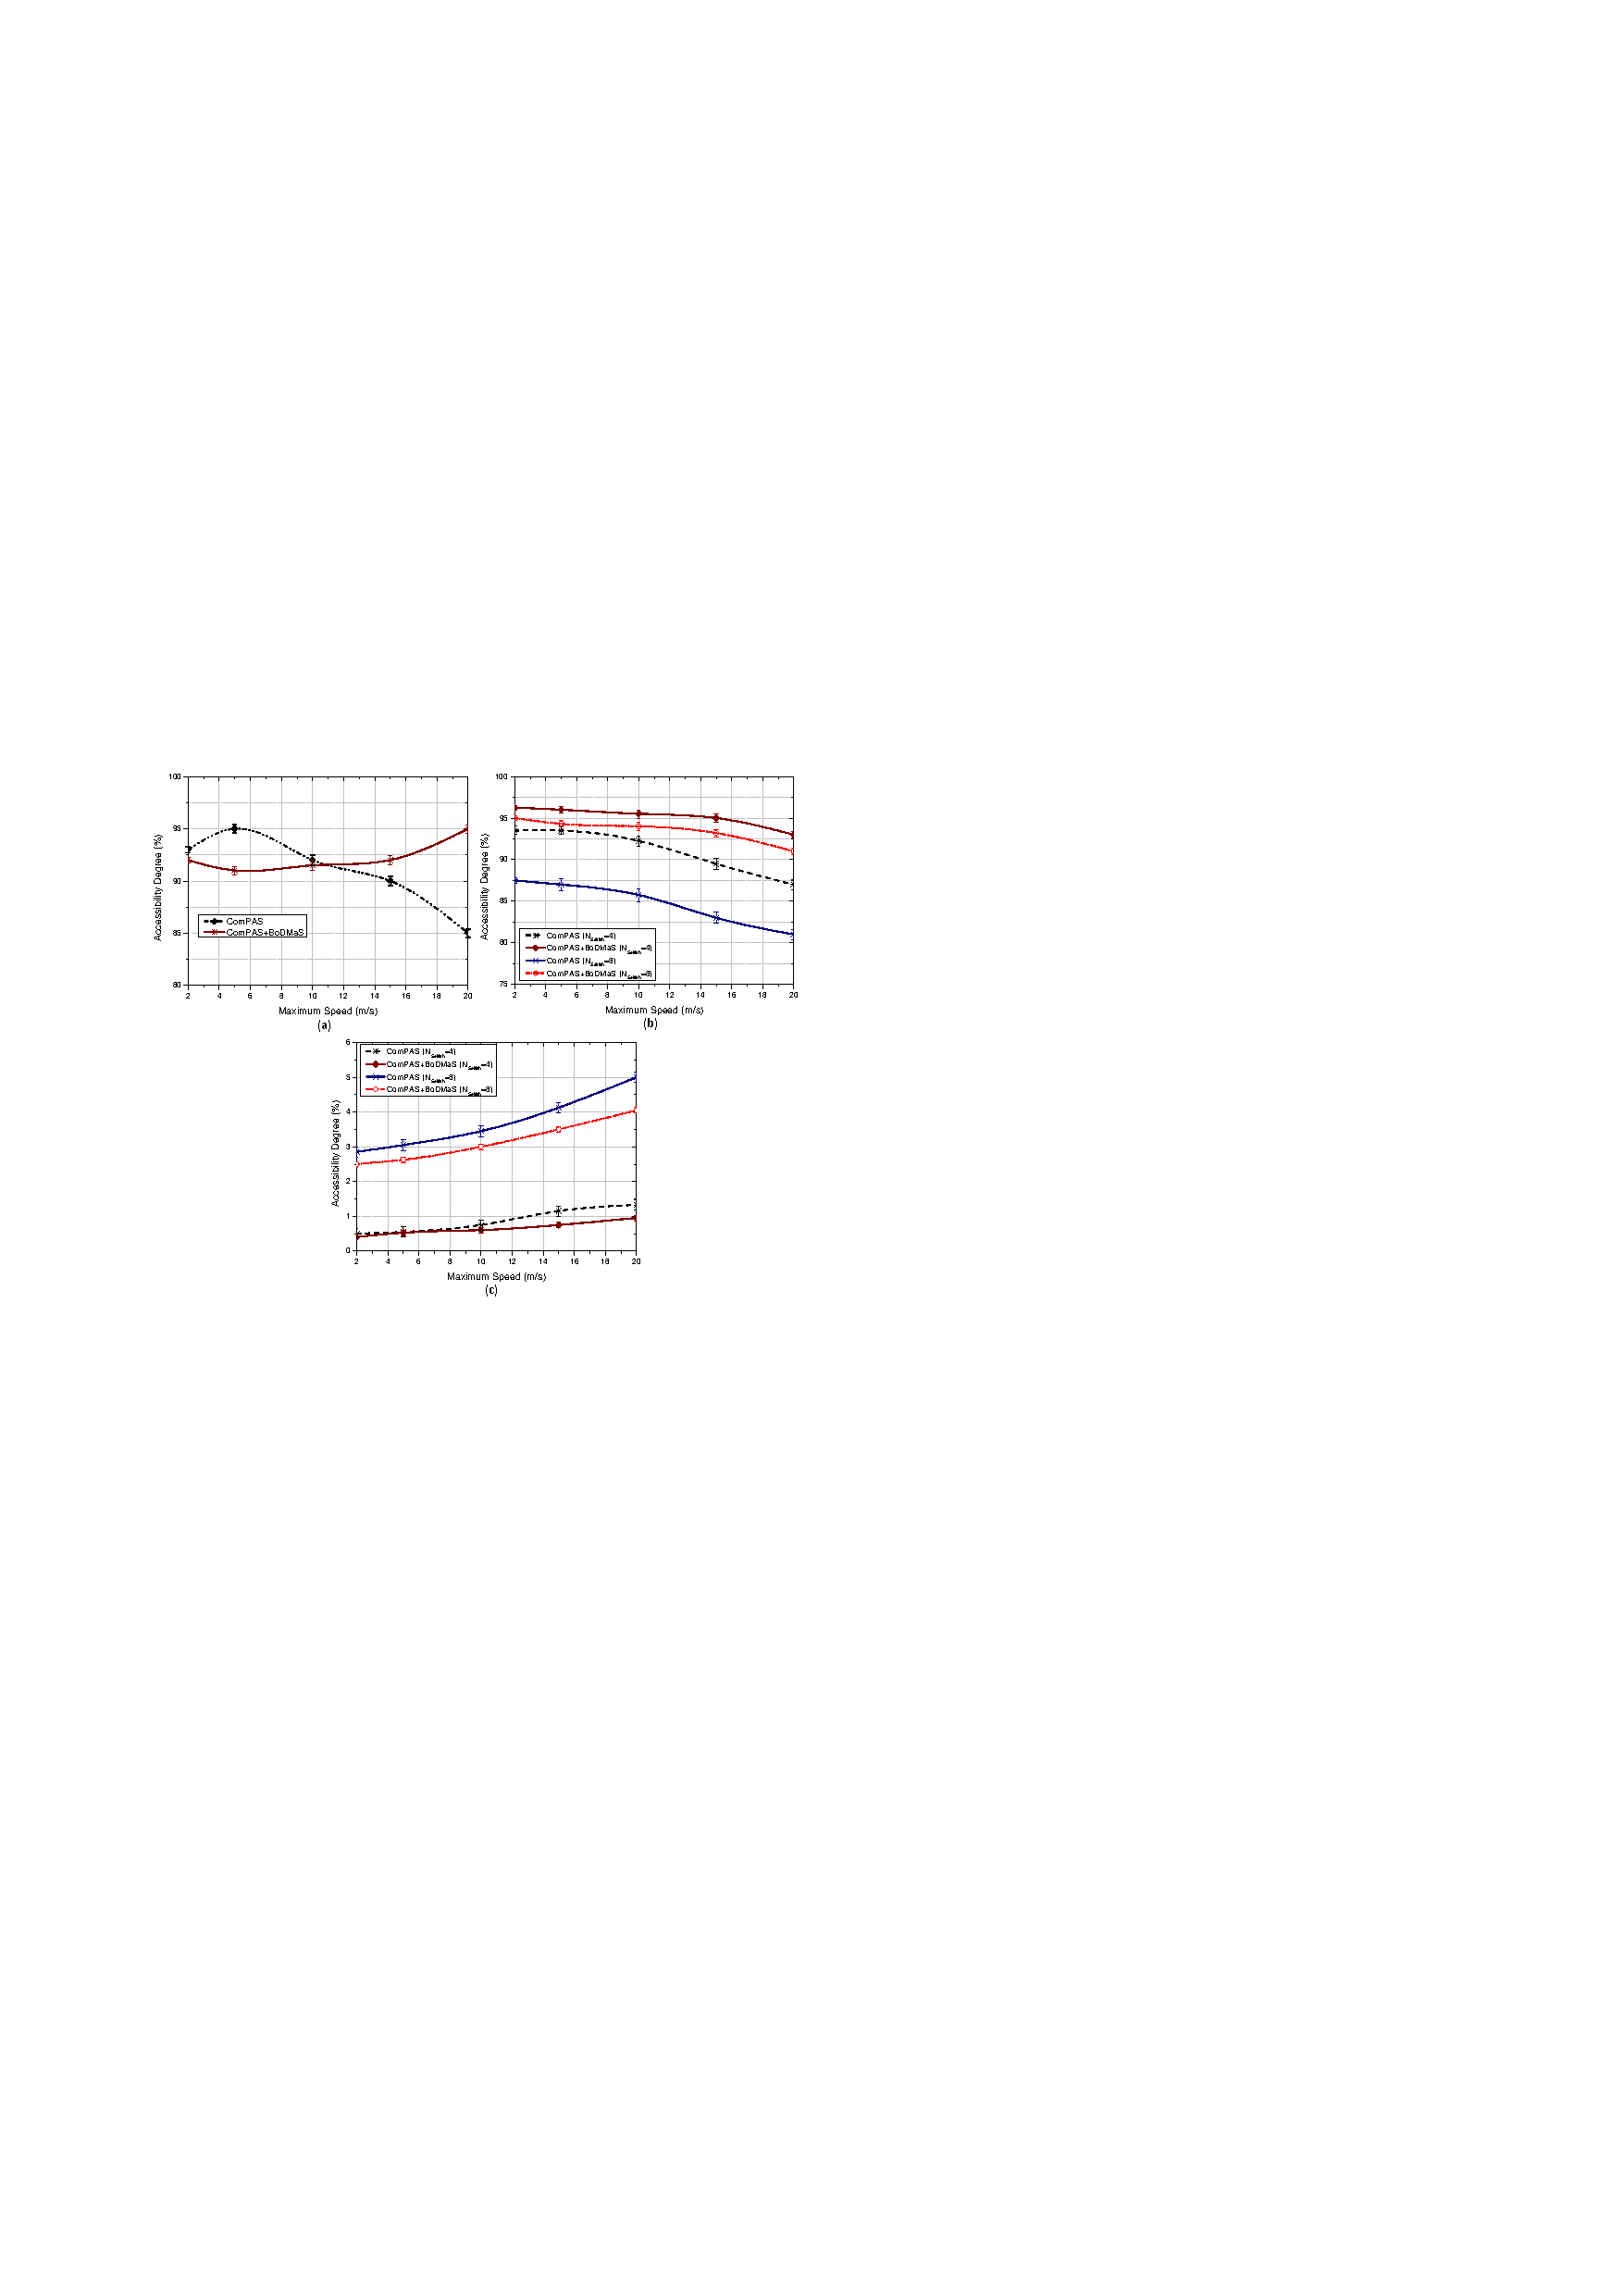
\includegraphics[width=0.95\textwidth]{Chap6-Fig6.pdf}
  \end{tabular}
  \caption{Accessibility degree for ComPAS$\uplus$BoDMaS and ComPAS; (a) without selfish users participation, and (b) with selfish users participation ($N_{Selfish}$ = 4 and $N_{Selfish}$ = 8) in update operations, (c) with selfish users participation ($N_{Selfish}$ = 4 and $N_{Selfish}$ = 8) in query operations.}
\end{center}
\end{figure}

Accessibility degree is the ratio of the number of successful access (query) requests to the number of all access requests issued which is an important metric for replication and reliability protocols. A replication method aims to increase the accessibility of data items in the network. Different from conventional static networks, in ASNETs achieving 100\% accessibility degree is nearly impossible due to mobility of nodes and changing network topology. To demonstrate effectiveness of integrated ComPAS and BoDMaS (ComPAS$\uplus$BoDMaS), we run simulation in two modes  for accessibility degree; firstly simulation in the presence of selfish users and secondly, simulation in the absence of selfish users. The results of our performance evaluation are depicted in Fig. 6.6.

Results of accessibility degree in the absence of selfish users for both ComPAS and ComPAS$\uplus$BoDMaS are illustrated in Fig. 6.6(a) when maximum speed increases from 2 to 10 m/s.  In low speed from 2 to 15 m/s, ComPAS$\uplus$BoDMaS does not shows positive accessibility improvement. However, as the maximum speed grows to 20 m/s, the difference is higher (from 85\% to 95\% for ComPAS and ComPAS$\uplus$BoDMaS, respectively). Evaluation results advocate that the proposed scheme shows a better performance than ComPAS in high speed mobilities, because, distant BoDMaS users (from other users) and those with smaller social willingness (connectivity) are not chosen to participate in the replica query and update operations. This also shows that the proposed scheme enforces a minimal trade-off between accessibility and security.

As displayed in Fig. 6.6(b), the use of BoDMaS shows an average improvement of 4.31\% and 8.94\% compared to the accessibility degree obtained by ComPAS without using BoDMaS in update operations for selfish users' participation with 4 and 8 respectively. The numbers of participating selfish users and the maximum speed have visible influence in ComPAS$\uplus$BoDMaS for both operations (Figs. 6.6(b) and (c)), when compared to ComPAS. However, as depicted in Fig. 6.6(c), with low variation, the evaluation presents lower results than ComPAS for query operations. This is because effect of selfishness for accessibility degree is less on query operations as compared to update operations. In the remaining part of this section, we focus on demonstrating the effectiveness of the proposed scheme in terms of true and false detection rates for query and update operations as well as network load balance.

\subsection{Detection Rate}\label{Chap6_05_02}
\esubsection{Detection Rate}
Detection rates obtained by BoDMaS for selfish user in query and update operations are illustrated in Figs. 6.7(a)-(c) and 6.8(a)-(c), respectively. TDR for query and update operations are presented in Figs. 6.7(a) and 6.8(a), while FDR (FN and FP) for query and update operations are presented in Figs. 6.7(b) \& (c) and 6.8(b) \& (c), respectively.

\subsubsection{Query Operation}\label{Chap6_05_02_01}
%\esubsubsection{Query Operation}
As depicted in Fig. 6.7(a), number of selfish users have visible impacts on detection rate results. For instance,  with 2 selfish users ($N_{Selfish}$ = 2) at a maximum speed of 2m/s, 5m/s, 10m/s, 15m/s and 20 m/s, the true detection rate for query operation is around 95.5\%, 95.6\%, 96\%, 95.8\% and 95.35\%, respectively. With 16 selfish users' participation ($N_{selfish}$ = 16) at a maximum speed of 2m/s, 5m/s, 10m/s, 15m/s and 20 m/s, the true detection rate for query operation is around 92.25\%, 92.5\%, 92.1\%, 91.625\% and 91\%, respectively. However, the TDR of selfish users in query operation for all the cases is higher than 90.95\%, because the proposed algorithm continuously assesses the selfish behavior of users and changes its status from selfish to cooperative when user resumes collaboration in forwarding query operations. Fig. 6.7(b) displays 1.2\% lower FN detection rate which shows very small error rate in mistakenly classifying selfish users as cooperative. This is due to the BoDMaS feature that counts $A_i$, individually. Furthermore, we evaluate FP detection rate as shown in Fig. 6.7(c) which is also a relatively small rate in mistakenly detecting cooperative users as selfish.
\begin{figure}[t]
\begin{center}
  \begin{tabular}{c}
  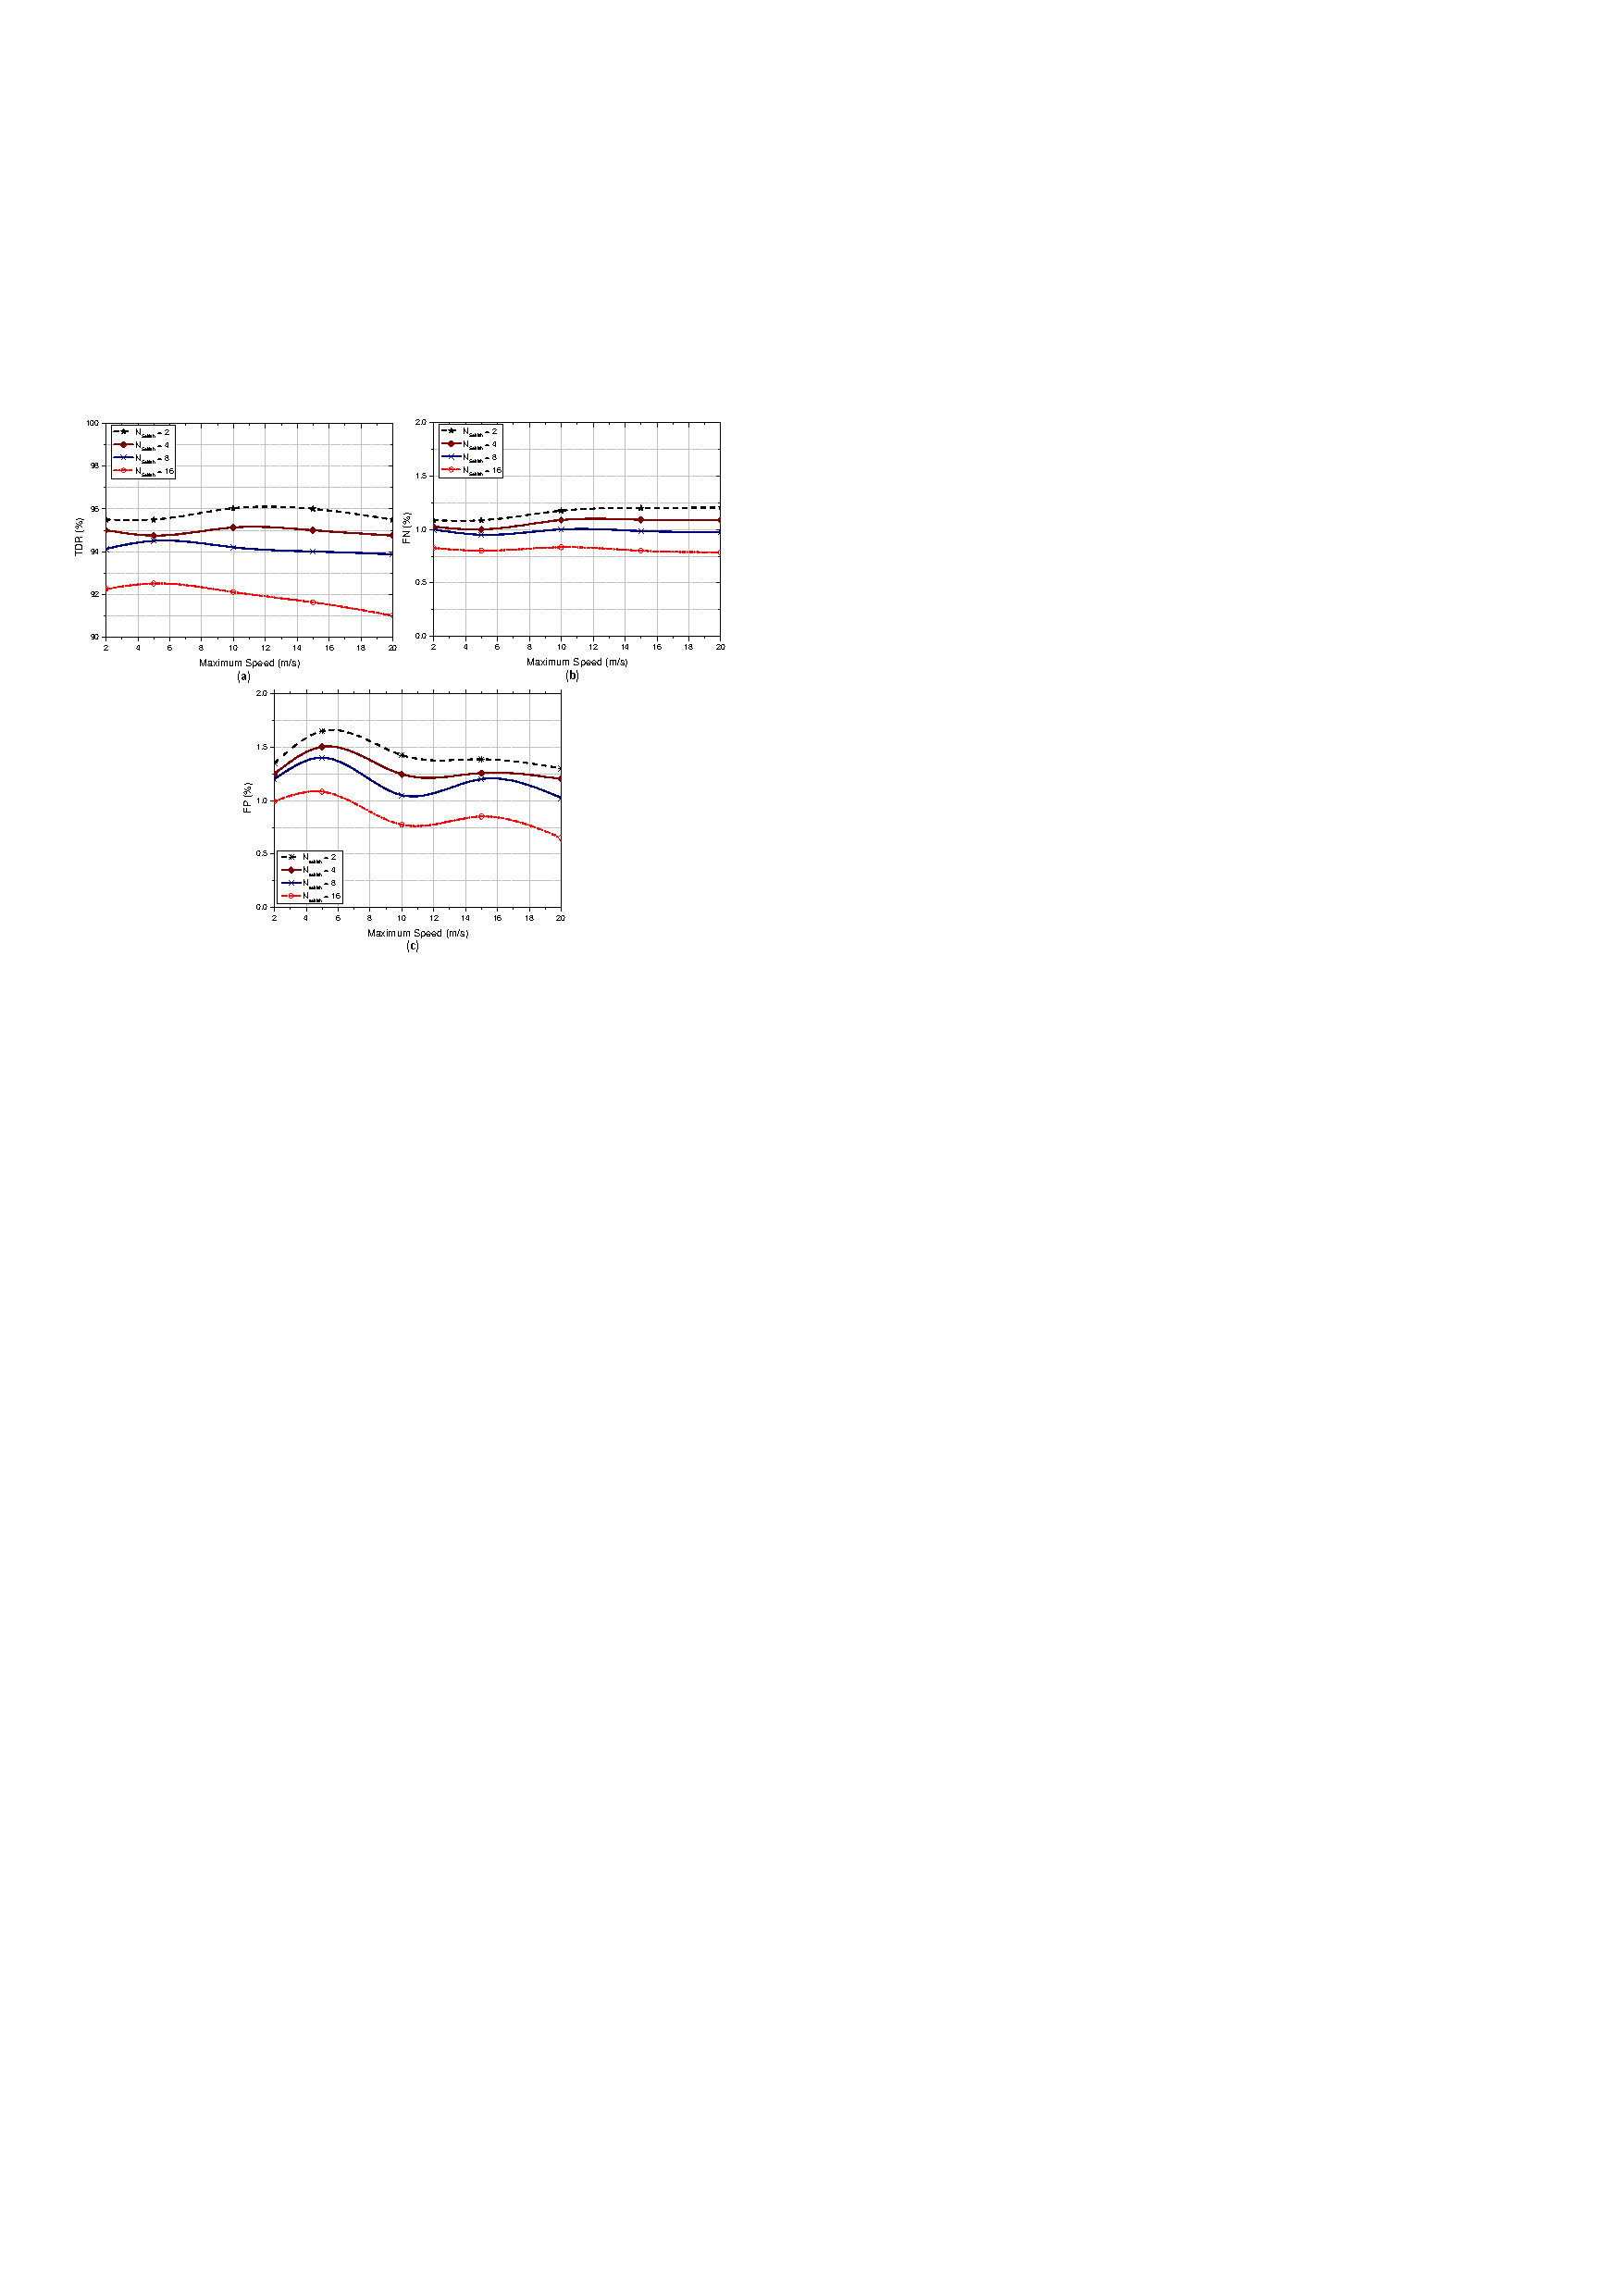
\includegraphics[width=0.95\textwidth]{Chap6-Fig7.pdf}
  \end{tabular}
  \caption{BoDMaS detection rate of selfishness in query operations; (a) true detection rate (TDR), (b) false negative (FN), and (c) false positive (FP).}
\end{center}
\end{figure}

\subsubsection{Update Operation}\label{Chap6_05_02_02}
%\esubsubsection{Update Operation}
\begin{figure}[t]
\begin{center}
  \begin{tabular}{c}
  \includegraphics[width=0.95\textwidth]{Chap6-Fig8.pdf}
  \end{tabular}
  \caption{BoDMaS detection rate of selfishness in update operations; (a) true detection rate (TDR), (b) false negative (FN), and (c) false positive (FP).}
\end{center}
\end{figure}
In order to evaluate the efficiency of BoDMaS during update operation, we simulated operation in varied scenarios with different numbers of selfish users ($N_{Selfish}$ = 2, 4, 8 and 16) and analyzed detection rates (i.e., TDR and FDR). Results of our simulation are presented in two ways as shown in Figs. 6.8(a)-(c).  The detection rates with 2m/s, 5m/s, 10m/s, 15m/s and 20m/s on update operations are very similar to query operation. We depict them as small charts inside each chart in Fig. 6.8.
Therefore, we suspected how the result shows similarity for these two different operations while there are some users which might be malicious to be considered as selfish due to the timeout manipulation on the data.

Timeout manipulation is considered in our scheme and it is experienced in update operations only. In order to verify this, we run the scheme with participation of 2, 4, 8 and 16 selfish users' for continuous maximum speeds in a range of 2m/s and 20m/s. For all the detection rates this behavior (existence of timeout manipulation on update operation) proved to be true, as seen in Figs. 6.8(a)-(c). While TDR is higher than 90\% for almost all cases, there is a point where this rate goes down below 90\% with a speed of around 18m/s as shown in Fig. 6.8(a). This is because some users are not considered as selfish, but have the behavior of malicious users happen partly as a timeout manipulation. The same is repeated for false negative and false positive detection rates as depicted in Figs. 6.8(b) and (c), respectively. This is an evidence to consider and improve the consistency of our scheme in terms of detection rates for update operations. Moreover, BoDMaS obtained good detection rates for update operations with the specified maximum mobility of users in the scenario.

\subsection{Network Load Balance}\label{Chap6_05_03}
\esubsection{Network Load Balance}
\begin{figure}[t]
\begin{center}
  \begin{tabular}{c}
  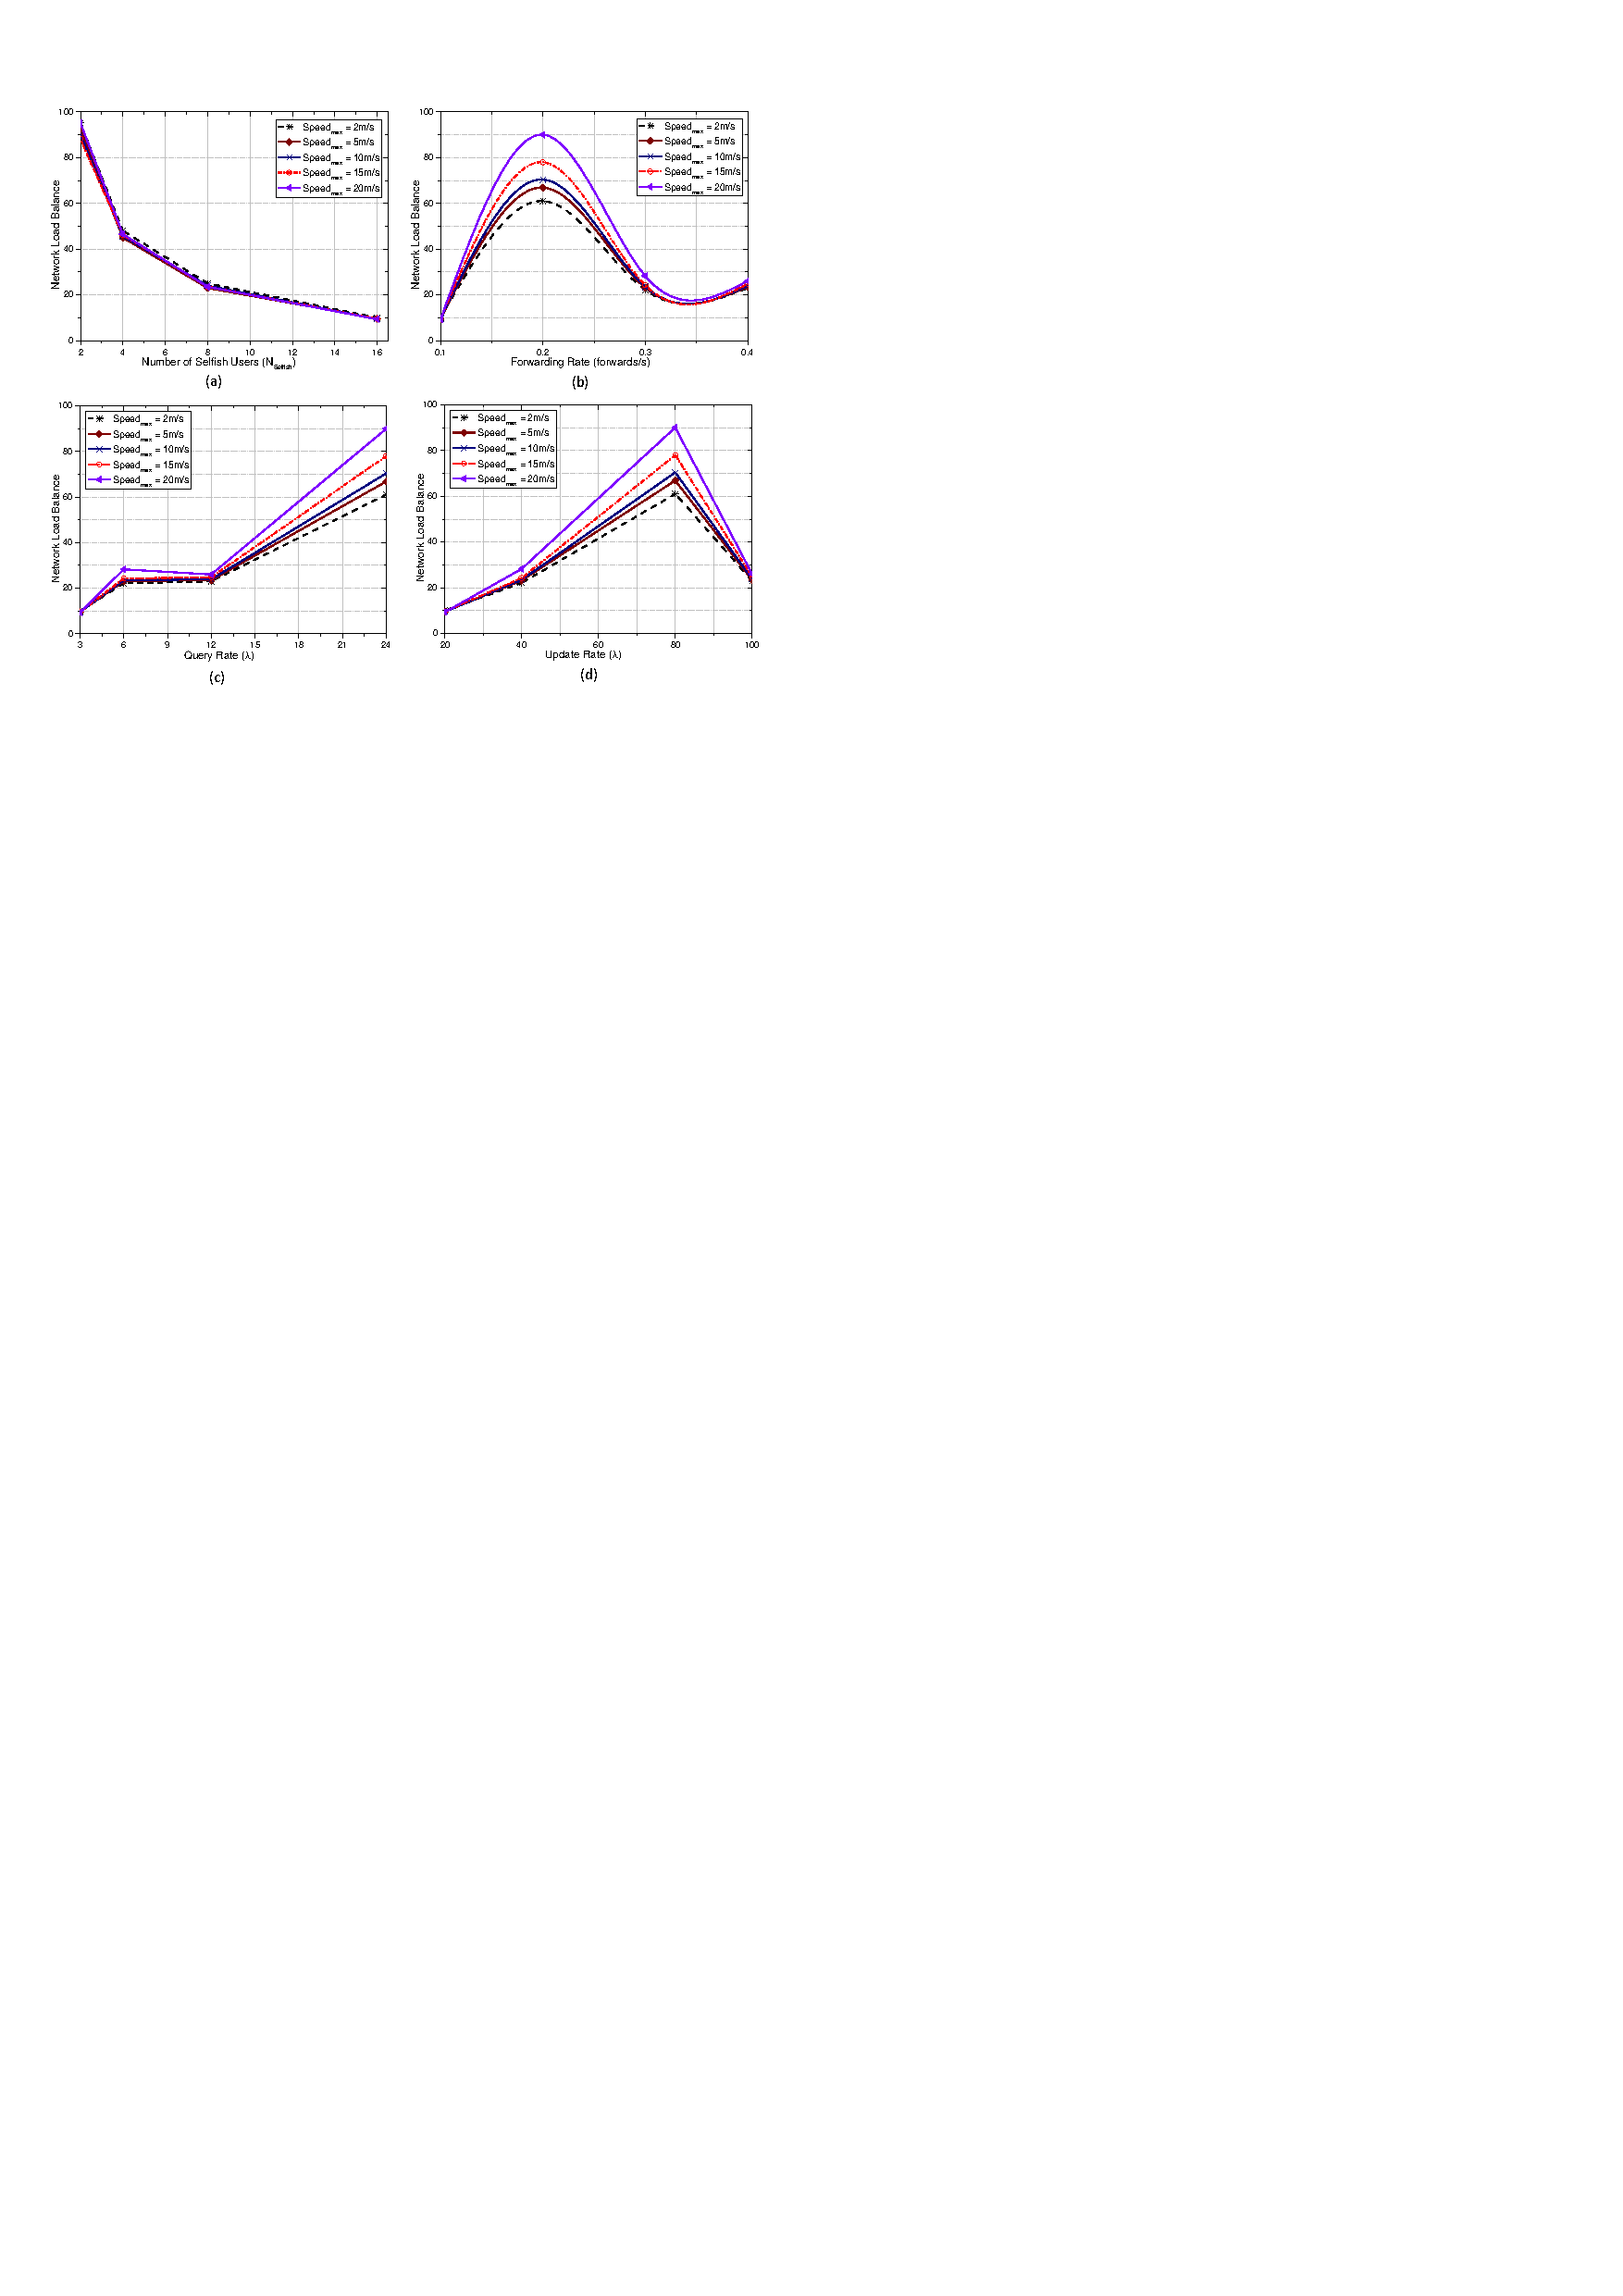
\includegraphics[width=0.9\textwidth]{Chap6-Fig9.pdf}
  \end{tabular}
  \caption{BoDMaS network load balance efficiency in terms of; (a) number of selfish users ($N_{Selfish}$), (b) forwarding rate, (c) query rate, and (d) update rate.}
\end{center}
\end{figure}

Network load balance is the ability of our algorithm to balance traffic across users (including the operations) of network scenario without applying load balancing and fairness mechanisms. The evaluations of network load balance are presented in four ways as shown in Figs. 6.9(a)-(d). The effect of number of selfish users on the network load balance is depicted in Fig. 6.9(a). The network load balance decreases from 90\% to 15\% with the increase in the numbers of selfish users participation (from $N_{Selfish} = 2$ to $N_{Selfish}=16$) due to resource wastage of selfish users. However, network load balance doesn't change when speed changes from 2m/s to 20m/s, which means that network load balance in BoDMaS is not much influenced by differences in low and high user mobility. The main reason for this anomaly is that the participation of selfish users has a dominating effect in most cases than the speed of these users. As described at the very beginning of this section, we set threshold values for forwarding, query, and update rates. Using Figs. 6.9(b)-(d), we demonstrate the probability that how our choices of the values are comparably successful based on the network load balance even if we only compare with very few values. Based on these observations, the ability of our algorithm to balance traffic across users is successful using the threshold values; forward threshold of 0.2, query rate of 24 and update rate of 80 as shown in Fig. 6.9(b), Fig. 6.9(c) and Fig. 6.9(d), respectively. Moreover, unlike Fig. 6.9(a), the network load balance shows an increasing behavior when the mobility of users (speed) is higher.

Overall, according to the simulation results shown in Figs. 6.6 - 6.9, we have demonstrated the effectiveness of our algorithm in terms of accessibility degree, detection rates (true detection rate and false detection rate) and network load balance.

\section{Summary}\label{Chap6_06}
\esection{Summary}
In this chapter, we have demonstrated the feasibility and significance of integrating social willingness with quorum sensing (a well-known bio-inspired mechanisms) to detect and counteract selfishness in ASNET. We introduced BoDMaS, an algorithm that assesses user's social tie with quorum sensing to classify users as either selfish or cooperative. BoDMaS exploits user classification results to inhibit selfish users from performing operation in network and also alert cooperative users to stop forwarding requests to selfish users. For effective evaluation of BoDMaS, we integrate it with ComPAS (a socially-aware replication system that ensures high availability in ASNETs, as proposed in chapter \ref{chap02}) and run series of simulations in an academic conference and analyzed three metrics, namely accessibility degree, detection rates, and network load balance. The evaluation results yield high TDR, low FN and FP with fast detection speed leading to enhanced data replication in ASNETs which are evidences of BoDMaS effectiveness. Moreover, BoDMaS is efficient in terms of the ability to balance traffic in varied network scenarios.

\chapter{Conclusion and Future Work}\label{Chap7}
\echapter{Conclusion and Future Work}

\section{Conclusion}\label{Chap7_01}
\esection{Conclusion}
Data management in ASNETs is challenging because it is different from the traditional data management in wired networks in that disconnections are the norm instead of the exception. In this dissertation, we have covered data management protocols in ASNETs with the exploitation and adaptation of different social features and techniques. First, we proposed an ASNET middleware framework which can be considered as an insight we revealed to serve as a basis for the design of middleware protocols in this emerging paradigm. There are no standard design approaches used to design middleware protocols in ASNETs. This dissertation defines and describes a number of approached and techniques that can be used for the design of efficient protocols. Then, we provided three data management protocols for ASNETs, which maximizes data availability, balances the load fairly and excludes selfish users, respectively.

Specifically, we proposed a data replication protocol based on partitioning of social community combined with social relationship and a user level replication so that data availability for all users is guaranteed. The system gives a fixed number of replicas required for each user that results in an efficient replication solution, particularly in terms of read cost. We also introduced the importance of integrating filter-based and multicast-based publish/subscribe systems for designing a community-based load balancing method. We have specifically proposed a community-based load balancing method combined with fault-tolerance techniques that minimizes overloaded brokers by distributing the event publication load among brokers. We employ an offloading mechanism and interest based similarity filter replication, to reduce the overall load distribution among communities and distribute and balance the load among brokers in a community, respectively. Finally, we proposed a bio-inspired protocol to detect and classify users to be either selfish or cooperative in ASNETs. This protocol gives each user the autonomy to take action against selfish users and it exploits out data replication protocol as a data management model. Simulation evaluations are conducted using synthetic traces to show that the proposed protocols are comparatively better than the existing one.

\section{Future Work}\label{Chap7_02}
\esection{Future Work}
Looking into the future, I will continue the research on the ASNET middleware problems. We believe that, there is still a lot that needs to be investigated, social awareness, learning and acquisition levels of the middleware framework, for example. To this end, we go one step further to envisage more state-of-the-art middleware solutions to be developed in the future. Extensions of this work should focus on two major research points.

\begin{enumerate}
    \item {Design a filter replication mechanism to regulate communication overhead while achieving reliability using fault-tolerance. We will also work on reducing misbehaving nodes in a community as they pose a profound negative impact on load balancing. This would allow a more uniform, efficient and reliable service. Co-Lab can also be adapted to integrate considerations for the mobility of nodes in the community, so as to further reduce the overhead incurred by the links between brokers and subscribers.}
    \item {Investigate the data management scheme for different parameters such as maximum speed and percentage of selfish users to enhance the protocol. A possible future work can be on the consideration of malicious users that inject malicious data to the process and evaluate the effectiveness of our system under expanded network environments. It is also possible to consider the load of users in the model so that they will have fair distribution of operation requests.}
\end{enumerate}

Another interesting future research direction would be data forwarding and routing protocols which would consider users online and dynamic social behaviors. Most of the existing socially-aware routing protocols prioritize interest similarity to enhance the performance of the protocol. Such protocols could be less efficient than routing protocols that consider users dynamic behavior in networks with high user mobility or high traffic rates. One example of future work can be on the coordination of the data replication, load balancing and routing mechanisms and investigates resource allocation and overhead among them, which has not been studied before.



\cleardoublepage
%\backmatter
\chapter*{Abstract of Innovation Points}
\addcontentsline{toc}{chapter}{Abstract of Innovation Points}
\addcontentsline{toe}{chapter}{Abstract of Innovation Points}
The abstract of innovation points in this dissertation include the following:
\begin{enumerate}
    %\item {Propose an ASNET middleware framework that integrates layers from sensing level to application level. It helps to provide the background for design and evaluation of the middleware protocols.}
    \item {Propose ComPAS - a replica allocation mechanism to maximize data availability in ASNETs. We presented the significance of exploiting social features such as friendship and group mobility modeling in allocating replicas of user data. The main aim of this replication protocol is to find an effective and reliable way to store fixed numbers of replicas for each user's data on the storage space of other communities. The decision on the number of replica for each user depends on the replication budget and its desired availability or accessibility. By placing the replica at the storage space of most neighbors, they benefit from this replica when they issue a read query.}
    \item{Propose a community-based load balancing and fairness approach called Co-Lab, which enhances the performance of the data management middleware. This solution exploits offloading and filter replication at the inter-community and intra-community levels, respectively. This facilitates the dynamic dissemination and forwarding of pub/sub services among brokers. Moreover, the exploitation of interest similarity and integration filter-based functionality within each multicast group helps to achieve fair load distribution among each broker and reduce the overall load distribution.}
    \item{Propose BoDMaS - a biologically inspired algorithm to detect and mitigate the impact of selfish users in replication process. Its design integrates user willingness with bacteria social coordination mechanism that aims to identify and counterpart selfishness in ASNETs. BoDMaS performs continuous user assessment, classification, selection of users to detect, and take actions to deny the involvement of selfish users in communication. As a proof of concept and for performance evaluation, BoDMaS is employed in a simulated academic conference event to offer autonomy to mobile participants in identifying and excluding selfish users from their network.}
\end{enumerate}

\cleardoublepage
% References
\twelve
\bibliographystyle{GBT7714-2005NLang}
\phantomsection
\addcontentsline{toc}{chapter}{References}
\addcontentsline{toe}{chapter}{References}
\bibliography{body/my_references}
\cleardoublepage

%\defaultfont
%\begin{appendix}
%   \input{appendix/chapA}
%\end{appendix}
%\cleardoublepage

\defaultfont
% Innovation

% Appendix
%\include{appendix/appendix}
%\cleardoublepage

% Published Academic Papers
\chapter*{\hfill Published Academic Theses during PhD Period \hfill}
\addcontentsline{toc}{chapter}{Published Academic Theses during PhD Period}
\addcontentsline{toe}{chapter}{Published Academic Theses during PhD Period}

\renewcommand{\labelenumi}{[\arabic{enumi}]}
\section*{Journal Papers}
\begin{enumerate}
\item
Feng Xia, \textbf{Ahmedin Mohammed Ahmed}, Laurence Tianruo Yang, Zhongxuan Luo. Community-based Event Dissemination with Optimal Load Balancing, IEEE Transactions on Computers, 2014, DOI: 10.1109/TC.2014.2345409. (Served as Chapter 5 of this dissertation)

\item
\textbf{Ahmedin Mohammed Ahmed}, Tie Qiu, Feng Xia, Behrouz Jedari, Saeid Abolfazli. Event-based Mobile Social Networks: Services, Technologies and Applications, IEEE Access, vol. 2, no. 500-513, 2014. (Served as Chapter 2 of this dissertation)

\item
Feng Xia, \textbf{Ahmedin Mohammed Ahmed}, Laurence Tianruo Yang, Jianhua Ma, Joel Rodrigues. Exploiting Social Relationship to Enable Efficient Replica Allocation in Ad-hoc Social Networks, IEEE Transactions on Parallel and Distributed Systems, vol. 25, no. 12, pp. 3167-3176, 2014. (Served as Chapter 4 of this dissertation)

\item
Hannan Bin Liaqat, Feng Xia, Qiuyuan Yang, Zhenzhen Xu, \textbf{Ahmedin Mohammed Ahmed}, Azizur Rahim. Bio-inspired Packet Dropping in Socially-aware Ad-hoc Networks, International Journal of Communication Systems, 2014, DOI: 10.1002/dac.2857.

\item
Feng Xia, Li Liu, Jie Li, \textbf{Ahmedin Mohammed Ahmed}, Laurence Tianruo Yang, Jianhua Ma. BEEINFO: Interest-based Forwarding Using Artificial Bee Colony for Socially-aware Networking, IEEE Transactions on Vehicular Technology, 2014, DOI: 10.1109/TVT.2014.2305192.

\item
Li Liu, Qiuyuan Yang, Xiangjie Kong, Hannan Bin Liaqat, \textbf{Ahmedin Mohammed Ahmed}, Nakema Deonauth, Feng Xia. Com-BIS: A Community-based Barter Incentive Scheme in Socially Aware Networking, International Journal of Distributed Sensor Networks, Accepted for Publication, 2014.

\item
Hannan Bin Liaqat, Feng Xia, Jianhua Ma, Laurence Tianruo Yang, \textbf{Ahmedin Mohammed Ahmed}, Nana Yaw Asabere. Social Similarity-aware TCP with Collision Avoidance in Ad-hoc Social Networks, IEEE Systems Journal, 2014, DOI: 10.1109/JSYST.2014.2305191.

\item
Feng Xia, Nana Yaw Asabere, \textbf{Ahmedin Mohammed Ahmed}, Jing Li and Xiangjie Kong. Mobile Multimedia Recommendation in Smart Communities: A Survey, IEEE Access, vol.1, pp.606-624, 2013.

\end{enumerate}

\section*{Conference Papers}
\begin{enumerate}
\item
\textbf{Ahmedin Mohammed Ahmed}, Feng Xia, Qiuyuan Yang, Hannan Bin Liaqat, Zhikui Chen, Tie Qiu. Bacteria Inspired Mitigation of Selfish Users in Ad-hoc Social Networks, The 15th ACM International Symposium on Mobile Ad Hoc Networking and Computing (MobiHoc), Philadelphia, PA, USA, August 11-14, 2014. (Served as Chapter 6 of this dissertation)

\item
\textbf{Ahmedin Mohammed Ahmed}, Qiuyuan Yang, Nana Yaw Asabere, Tie Qiu, Feng Xia. ComPAS: Maximizing Data Availability With Replication in Ad-hoc Social Networks, The 23rd International World Wide Web Conference (WWW), Poster Track, Seoul, Korea, April 7-11, 2014. (Served as Chapter 4 of this dissertation)

\item
\textbf{Ahmedin Mohammed Ahmed}, Feng Xia, Nana Yaw Asabere, Hannan Bin Liaqat, Jie Li. Social Community-Partition Aware Replica Allocation in Ad-hoc Social Networks, in Proceedings of IEEE International Conference on Cyber, Physical and Social Computing (IEEE CPSCom), pp. 834-841, Beijing, China, Aug 21-23, 2013. (Served as Chapter 4 of this dissertation)

\item
Hannan Bin Liaqat, Qiuyuan Yang, \textbf{Ahmedin Mohammed Ahmed}, Zhenzhen Xu, Tie Qiu, Feng Xia. A Social Popularity Aware Scheduling Algorithm for Ad-hoc Social Networks, The 11th International Joint Conference on Computer Sciences and Software Engineering (JCSSE), Pattay City, Thailand, May 14-16, 2014.
\end{enumerate}

\section*{Book Chapter}
\begin{enumerate}
\item
Behrouz Jedari, Feng Xia, \textbf{Ahmedin Mohammed Ahmed}, Poria Pirozmand, and Yashar Najaflou. Chapter 11: Using Social Network Analysis (SNA) to Design Socially Aware Network Solutions in Delay-tolerant Networks (DTNs), in: Advances in delay-tolerant networks (DTNs), edited by J.J.P.C Rodrigues, Woodhead Publishing Series in Electronic and Optical Materials: Number 67, 2014, DOI: 10.1533/9780857098467.2.200.
\end{enumerate}

\section*{Papers Under Review}
\begin{enumerate}

\item
\textbf{Ahmedin Mohammed Ahmed}, Feng Xia, Runhe~Huang, Jianhua Ma. Middleware for Ad-hoc Social Networks: Design Challenges, IEEE Communications Magazine. (Served as Chapter 3 of this dissertation)(Second round review after Major Revision)

%\item
%\textbf{Ahmedin Mohammed Ahmed}, Feng Xia, Jun Zhang, Saeid Abolfazli, Zohreh Sanaei. BoDMaS: Bio-inspired Detection and Mitigation of Node Selfishness in Ad-hoc Social Networks, IEEE Transactions on Human Machine Systems. (Served as Chapter 6 of this dissertation)

\item
Behrouz Jedari, Feng Xia, \textbf{Ahmedin Mohammed Ahmed}, Jun Zhang. A Survey on Routing and Data Dissemination in Opportunistic Mobile Social Networks, Journal of Network and Computer Applications.

%\item
%Feng Xia, Jie Li, Qiuyuan Yang, Jiannong Cao, Li Liu, \textbf{Ahmedin Mohammed Ahmed}. Data Dissemination Using Interest Tree in Socially Aware Networking, IEEE Transactions on Parallel and Distributed Systems.

\item
Jie Li, Feng Xia, Li Liu, \textbf{Ahmedin Mohammed Ahmed}, Hannan Bin Liaqat, Zhenzhen Xu. Geo-Social Distance Based Data Dissemination for Socially Aware Networking, IET Networks.

\item
Hannan Bin Liaqat, Feng Xia, \textbf{Ahmedin Mohammed Ahmed}, Li Liu, Zhenzhen Xu, Xiangjie Kong. User Popularity-based Packet Scheduling for Congestion Control in Ad-hoc Social Networks, Journal of Computer and System Sciences.

\end{enumerate}




\cleardoublepage

% Acknowledgement
\chapter*{\hfill Acknowledgement \hfill}
\addcontentsline{toc}{chapter}{Acknowledgement}
\addcontentsline{toe}{chapter}{Acknowledgement}

Studying for a PhD and moving to a foreign country has certainly been a valuable, exciting and an enriching experience, both personally and professionally, but it has been very challenging as well. I could not have succeeded without the advice, support and influence of many colleagues, friends and family. My thanks are due first and foremost to my advisor Prof. Feng Xia, for being a consistent source of support and encouragement. He always provides me with great insight and useful advice whenever I need discussion. His motivation and drive for excellence set an excellent example for my PhD study and his guidance and help have made my Ph.D. program a challenging and productive one. His professional dedication and integrity with positive attitude will always been an inspiration to me. I will be forever grateful for his help. I will also like to thank Dr. Xiangjie Kong for all his help and assistance as a co-advisor.

During the whole period of my doctorate study, I have been immensely fortunate to work and co-author with many great individuals, notably, Prof. Laurence Yang, Prof. Jianhua Ma, Prof. Joel Rodrigues, Prof. Zhikui Chen, Prof. Zhongxuan Luo, Dr. Tie Qiu, Prof. Runhe Huang and Dr. Saeid Abolfazli. I am deeply indebted to members of DUT Phone Lab. I have received continuous help from Nana, Hannan, Dimitry, Behrouz, Jack, Wei Wang, Qiuyuan Yang, Haifeng Liu, Zhen Chen, Liu Li, Jing Li, Rina, Aziz and others in both academic and social sides. They made the time I spent working towards my Ph.D. full of excitement. I thank everyone for their kindness and help. I am grateful to Yancy Davis for his help on proofreading some of my works, Hayat Dino and Teshome Megersa for their help in proofreading this dissertation. I thank all of my PhD dissertation committee members and reviewers for their valuable comments and feedback. I cannot forget my friends and country-mates at Dalian and Chongqing who were always supportive of me.

Finally, I am grateful for my parents, Mohammed Ahmed and Lubaba Gizaw, and my brother Anewar. They gave me the strength to fight for my goals and ambitions, and provided me with indispensable support that was essential during the course of my study, and for the completion of this dissertation.


\vspace{1cm}
\hfill  Ahmedin~~~~~

\hspace{1cm}
\hfill November 2014~~~

\cleardoublepage

% About the Author
\chapter*{\hfill About the Author \hfill}
\addcontentsline{toc}{chapter}{About the Author}
\addcontentsline{toe}{chapter}{About the Author}

\begin{window}[0,r,{\mbox{\includegraphics[width=3cm]{author.jpg}}},{}]
\end{window}
\ltwelve
Name: Ahmedin Mohammed Ahmed

Gender: Male

Date of Birth: 06~October~1985

Nationality: Ethiopia

Research Direction: Ad-hoc social networks, mobile data management, middleware design

Resume:


\twelve
2003/9~-~2006/7~~~Bahirdar~University~~~~~~~~~~~~~~~~~~~~~~~~Computer~Science~~~~~~~~~~~~~~BSc \par
2009/9~-~2011/7~~~Chongqing~University~~~~~~~~~~~~~~~~~~~~~Software~Engineering~~~~~~~~MEng \par
2011/9~-~2014/11~Dalian~University~of~Technology~~~~Computer~Sci.~and~Tech.~~~~PhD

\cleardoublepage

% Copyright Aughorization
\chapter*{}
\addcontentsline{toc}{chapter}{大连理工大学学位论文版权使用授权书}
\addcontentsline{toe}{chapter}{Dalian University of Technology Doctoral Dissertation Copyright Use Authorization}
\addcontentsline{toe}{chapter}{大连理工大学学位论文版权使用授权书}

\renewcommand{\baselinestretch}{1.61}
\vspace{-0.48cm}
\eauthorization
\authorization
\cleardoublepage

\end{CJK*}
\end{document}

%%%%%%%%%%%%%%%%%% End of the file  %%%%%%%%%%%%%%%%%%%%%%%%
